\documentclass[a4paper,12pt]{scrbook}
\usepackage[utf8]{inputenc}
\usepackage[T1]{fontenc}
\usepackage{textcomp} % Degree symbol
\usepackage{xcolor} % Grey comments
\usepackage[colorlinks, allcolors=blue]{hyperref}
\usepackage{graphicx}
\usepackage{multirow} % Tables
\usepackage{appendix}
\usepackage{natbib}
\usepackage[super]{nth}
\usepackage{amsmath} % For declaring own arctan2
\DeclareMathOperator{\Arctan}{Arctan}
\usepackage{tikz} % Flowcharts
\usetikzlibrary{shapes,arrows, shadows, positioning}
\usepackage{caption}
\usepackage{subcaption} % Grid of figures
\usepackage{rotating} % Landscape page for grid of figures
\usepackage{adjustbox} % Scale table to height
%\usepackage{longtable} % Alternatively, cut table into two
% Formatting as per the template given
%\usepackage[top=1.25cm,bottom=1.25cm,inner=0.66cm,outer=0.53cm,foot=1.19cm,includeheadfoot]{geometry}
% Formatting with extra margins for sanity
\usepackage[top=1.25cm,bottom=1.25cm,inner=1.91cm,outer=1.91cm,foot=1.19cm,includeheadfoot]{geometry}
\usepackage{titling}
\usepackage{wrapfig}
\renewcommand{\familydefault}{\sfdefault}
\bibliographystyle{apalike}

%opening
\title{Fuzzy land cover classification method assessment using PROBA-V satellite data}
\author{Dainius Masili\=unas}
\date{\today}

% Flowchart blocks
\tikzstyle{block} = [rectangle, draw, fill=white, 
    text width=8em, text centered, rounded corners, minimum height=3em]
\tikzstyle{line} = [draw, -latex']
\tikzstyle{data} = [trapezium, trapezium left angle=70, trapezium right angle=110, text centered, draw,
    text width=6em, fill=gray!30, double copy shadow, minimum height=3em]
\tikzstyle{datasingle} = [trapezium, trapezium left angle=70, trapezium right angle=110, text centered, draw,
    text width=6em, fill=gray!30]
\tikzstyle{bigdata} = [trapezium, trapezium left angle=80, trapezium right angle=100, text centered, draw,
    text width=14em, fill=gray!30, double copy shadow, minimum height=3em]

\begin{document}

% Title page with its weird format

\begin{titlingpage}
  %\pagenumbering{roman}
  {\Large Centre for Geo-Information}\vspace{0.9cm}
  
  {\Large Thesis Report GIRS-2017-xx}\vspace{0.9cm}
  
  \hrule\vspace{1.1cm}
  
  {\bfseries \Large \MakeUppercase{\thetitle}}\vspace{2.0cm}
  
  \begin{wrapfigure}[1]{r}{0.55\textwidth}
    \begin{subfigure}[t]{0.25\textwidth}
      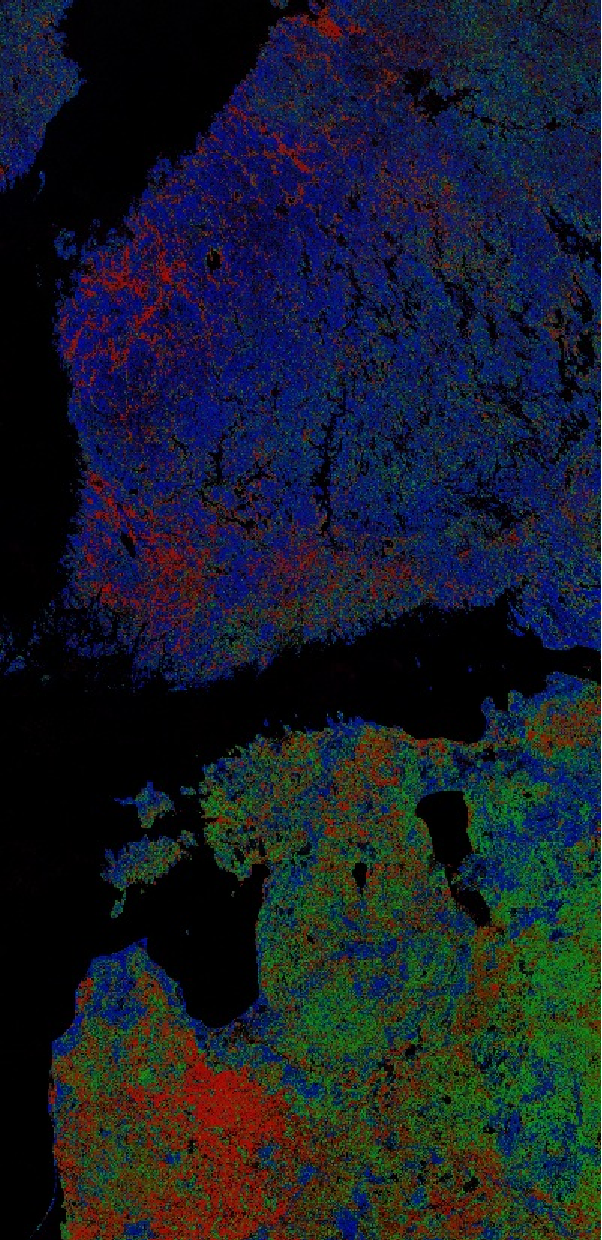
\includegraphics[height=9.5cm]{thesis-figures/figures-qgis/fulltile-rf}
    \end{subfigure}
    \begin{subfigure}[t]{0.25\textwidth}
      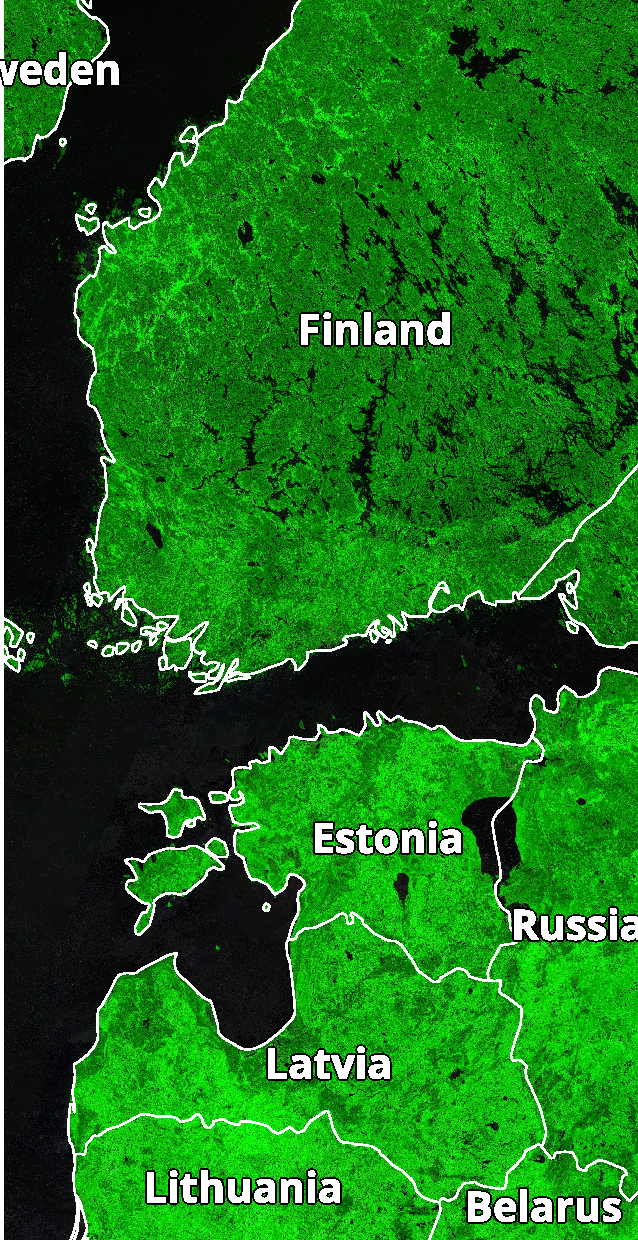
\includegraphics[height=9.5cm]{thesis-figures/aoi-blank}
    \end{subfigure}
    \vspace{-110pt}
  \end{wrapfigure}
  
  {\Large \theauthor} \vspace{5.9cm}
  
  \rotatebox{90}{\Large \thedate} \vspace{0.5cm}
  
  
\includegraphics[width=13cm]{wur-template/WUR_RGB_standard}
  
  \noindent\makebox[\textwidth]{\hspace*{\dimexpr\evensidemargin-\oddsidemargin}
\includegraphics[width=\paperwidth]{wur-template/image2}}
  
  \newpage % Second page
  \thispagestyle{empty}
  
  \begin{center}
  {\bfseries \Large \thetitle} \vspace{2.7cm}
  
  {\Large \theauthor} \vspace{1.1cm}
  
  {Registration number 93 04 07 546 120} \vspace{3.5cm}
  
  {\large \underline{Supervisors}:} \vspace{1.1cm}
  
  {Dr Jan Verbesselt}
  
  {Dr Nandin-Erdene Tsendbazar} \vspace{3.0cm}
  
  {A thesis submitted in partial fulfilment of the degree of Master of Science at Wageningen University and Research Centre, The Netherlands.} \vspace{3.7cm}
  \end{center}
  
  \begin{flushright}
    {\thedate}
  
    {Wageningen, The Netherlands}
  \end{flushright} \vspace{0.5cm}

    Thesis code number: GRS-80436
  
    Thesis Report: GIRS-2017-xx
  
    {Wageningen University and Research Centre}
  
    {Laboratory of Geo-Information Science and Remote Sensing}
\end{titlingpage}

\chapter*{Abstract}

Global land cover (GLC) classification is well established, and GLC products are used as input to a variety of scientific models. However, traditional GLC classification assumes that each pixel in a map can be classified into one of the predefined land cover classes. This is rarely the case in reality due to heterogeneity in land cover that results in a large number of mixed pixels. Such heterogeneity is better captured by fuzzy land cover classification, in which the proportions of each predefined land cover class is determined in each pixel. Methods used to produce hard GLC maps are not directly applicable to fuzzy land cover classification, and there exist a variety of methods that can be used for fuzzy classification tasks.

Four such methods, based on machine learning, were compared in this thesis: fuzzy \textit{c}-means, neural networks, random forest regression and multiclass gradient boosting. Data on land cover proportions for model training was gathered by image interpretation. Covariates for model prediction were derived from PROBA-V satellite sensor data (spectral bands, vegetation indices, time series parameters) and digital elevation models.

Results showed that all of the tested methods were similarly accurate. Random forest regression was the most accurate method, but also the slowest to predict. Neural networks was the fastest but least accurate method, and fuzzy \textit{c}-means was in between the two. Mean NDVI was the most important covariate, aspect and water mask were the least important.

\textbf{Keywords:} Fuzzy land cover classification, machine learning, random forest, gradient boosting, neural networks, fuzzy c-means, PROBA-V


%\maketitle
%\pagenumbering{arabic}
\setcounter{page}{3}

\tableofcontents

\chapter{Introduction}

Global land cover mapping is very important from an ecological and earth systems point of view. Land cover maps are used for a variety of applications, from estimating area covered by forests \citep{bartalev2014probavboreal} to air quality modelling \citep{wiedinmyer2006airquality}. In addition, land cover maps, especially those of fine spatial resolution, have the potential to be used for land cover change monitoring \citep{defourny2012cci}. This is important for a number of land cover classes. For instance, forests are an important terrestrial carbon sink in the global carbon cycle, with different forests having different carbon sink capacities \citep{pan2011large}. Knowing their distribution and changes over time allows for more accurate climate change modelling. Another land cover class, wetlands, is key for maintaining biodiversity due to the uniqueness of wetland ecosystems that allows rare and protected species to live there. Wetlands are protected globally by the Ramsar convention \citep{davis1994ramsar}.

The creation of a global land cover map from remote sensing data has been a goal of many different studies \citep{hansen2000hardtree}. Their results are nowadays freely available as satellite imagery products, such as Global Land Cover 2000 \citep{bartholome2005glc2000}, MODIS land cover \citep{friedl2010modis} and GlobCover \citep{arino2007globcover}. There are also maps based on the fusion of multiple other maps, like Geo-Wiki hybrid \citep{see2015hybrid}, and multiple sensors, like Land Cover CCI \citep{lccciguide} and GlobeLand30 \citep{chen2015globeland30}. However, these land cover maps all have certain drawbacks.

The first common drawback of current global land cover classification products is that their spatial resolution is low to medium. The majority of aforementioned land cover products are derived from MODIS and MERIS sensor data. The sensors are only capable of capturing images with the finest pixels representing 300 by 300 metre areas (at the equator). Recent advances in satellite sensors and computing power would allow for land cover classification at a higher spatial and temporal resolution. For example, at the moment the PROBA-V mission by the European Space Agency produces imagery with as fine as 100 by 100 metre pixels (with additional products also providing 300 by 300 metre and 1 by 1 kilometre pixel size for comparison with previous sensors) \citep{probavguide}. It is well-suited for time series analysis, because it has an archive that goes back to 2013, as well as a fast revisit time of 2 days for full global coverage (1 day for locations above 35\textdegree{} latitude) \citep{dierckx2014probav}.

The second drawback of current global land cover products is that their classification accuracy tends to be low, averaging at around 65\% \citep{tsendbazar2016integrating}. The third drawback is that all of these products use what is known as ``hard'' or ``crisp'' classification: each pixel is assigned to one particular land cover class only. The result of a hard classification is a thematic map. This classification type treats each pixel as homogeneous with regards to land cover, which is rarely the case in reality. In contrast, a ``fuzzy'' or ``soft'' classification, sometimes also called ``subpixel'' classification or ``linear mixture modelling'' \citep{Okeke2006fuzzyexponent} identifies the proportion of each land cover class within each pixel. The result of a fuzzy classification is one map per land cover class, showing the proportion of the pixel area covered by the land cover class.

Hard classification is not well-suited for coarse resolution imagery, due to a large proportion of mixed pixels in it (representing areas of mixed land cover), compared to endmember pixels (or pure pixels, which are dominated by a single land cover class). When hard classification is attempted on such imagery, the accuracy of the result can be no higher than the area fraction that the dominant land cover type of the pixel occupies \citep{latifovic2004accuracy}. There have been attempts at increasing accuracy by defining mosaic classes, such as mixed forests (50\% needleleaf and 50\% broadleaf trees), but it leads to a proliferation of classes that increases map complexity and still does not deal with the core problem, thus not improving the classification accuracy by much \citep{tsendbazar2016comparative}. In contrast, ``fuzzy'' or ``soft'' classification results in each pixel containing information about the proportion of each class within that pixel, therefore operating on sub-pixel scales. This has the advantage of representing land cover more accurately, and gives the ability to represent mosaic classes as a combination of pure classes instead. Since the output of fuzzy classification is essentially one raster per class, with smooth edges, it is suitable for more in-depth analysis and user-specific visualisation criteria \citep{tsendbazar2016integrating}. Despite that, hard classification is still the most often used classification type due to the number of algorithms developed for it, ease of storing the result (it is thematic and thus takes little storage space), displaying it in a single map (albeit in a less accurate fashion) and performing accuracy assessment.

There is a number of different classification algorithms, but only several of them are suitable to be used for fuzzy classification \citep{nath2014methods}. The two methods most commonly used in scientific literature are fuzzy \textit{c}-means and neural networks \citep{zhang2001fullyfuzzy}. Neural networks in particular are well-suited for fuzzy classification, since they allow multiple continuous output as well as input variables in a single model \citep{foody1997fuzzynnet}. Fuzzy \textit{c}-means, also known as fuzzy k-means or soft k-means, is a statistical method that relies on the proximity of pixels in feature space to class centroids, and thus is also suitable for fully fuzzy classification. However, since k-means is an unsupervised classification algorithm, the ability to make use of training data in fuzzy \textit{c}-means is limited to determining class centroids with more precision \citep{hengl2004fuzzycmeans}, and as such it is effectively similar to maximum likelihood classification.

In addition, any other algorithms that provide a measure of uncertainty about class membership can be used, such as the ratio of individual tree votes of random forest \citep{breiman2001random} or class probabilities in gradient boosting \citep{friedman2001gradientboost}. While classification uncertainty is not a direct measure of class membership \citep{sytze2000fuzzyset}, they are nonetheless correlated. As such, it has been used by numerous authors as a proxy indicator of class membership, achieving satisfactory classification accuracy \citep{foody2002accuracy}.

Furthermore, algorithms that can handle continuous variables, but only one response variable (such as random forest), can be used as well, by creating separate models for every class. This approach is called binary relevance \citep{karalas2016br}. Using this approach, the data needs to be post-processed after classification at a pixel level to conform to physical constraints (class membership must be between 0 and 100\% and sum up to 100\%). Random forest has been reported to give higher or equal accuracy results compared to other algorithms, like Support Vector Machines and individual decision trees, in hard classification scenarios using satellite imagery similar to that of PROBA-V \citep{duro2012algorithmcomparison}. Random forest regression was also shown to perform as well as other algorithms in fuzzy classification scenarios \citep{walton2008subpixelrf}, although it is used in much fewer studies on fuzzy classification than the other algorithms mentioned previously. Gradient boosting is an algorithm related to random forest, with the same advantages and disadvantages, but it is known to perform better in machine learning challenges \citep{chen2015higgs} and has not yet been tested on fuzzy land cover classification.

Accuracy assessment is rather straight-forward for hard classification: typically a confusion matrix is employed for this purpose, showing how many pixels (or in some cases how much area \citep{stehman2009sampling}) in the image have been classified correctly, and how many incorrectly. Such a matrix makes it simple to tell which classes are hard to discern from one another, as well as allows for deriving statistics such as users' accuracy, producers' accuracy, and overall accuracy \citep{foody1996fuzzyevaluation}, as well as variance if probability sampling was used. However, a standard confusion matrix is not applicable in the context of fuzzy classification, since misclassification in this case is not absolute, but rather a matter of degree \citep{foody2002accuracy}. Several solutions, such as distance \citep{foody1996fuzzyevaluation}, cross-entropy and mutual information \citep{lu2007methods} have been suggested as alternatives for fuzzy classification accuracy assessment.

Visualisation of the fuzzy classification results is also challenging, since each class effectively is a single-channel raster of its own. Three such classes can easily be combined into RGB channels for visualisation, but with more classes it is no longer possible. There have been attempts to develop a method based on the hue, saturation and intensity colour model to allow for a larger number of distinct classes to be visualised on a single raster \citep{hengl2004fuzzycmeans}. There is also a possibility of ``hardening'' the classification when high accuracy visualisation is not needed, and making use of multiple RGB rasters side-by-side when it is needed.

All in all, even though global land cover mapping has been a focus of many other studies, existing global land cover maps still have room for improvement. This can be achieved by using data from the sensors of newer satellites such as PROBA-V, as well as performing fuzzy classification as opposed to the traditional hard classification.

\chapter{Problem definition and research questions}

An important long-term goal of land cover mapping is to have a highly accurate fuzzy land cover classification method at a global scale. Since there are many different methods that could be used to achieve such a goal, and since the amount of data generated by satellites covering the entire world is enormous, this thesis focuses on comparing several different fuzzy classification methods on a subset of global imagery provided by the PROBA-V satellite.

PROBA-V is a relatively new satellite, with few studies using it for land cover classification so far. A number of studies have used simulated PROBA-V data in preparation for its launch \citep{stathakis2014probavurban,roumenina2013probavcrops,bartalev2014probavboreal}. After launch, most studies have focused on its potential for crop classification \citep{roumenina2015probavcrops,durgun2016crop,lambert2016cropland}. All of these studies have only used the traditional hard classification. As such, the potential of using PROBA-V data for fuzzy classification in order to obtain a more accurate representation of land cover at global scale has never been tested before.

Another problem of land cover classification is that there is high disagreement between different land cover products on mixed classes, such as mixed forests \citep{Herold2008lccomparison}. Mixed forests and wetlands are challenging to detect and classify using hard classification and optical remote sensing data, so it is important to check how well large-scale fuzzy classification performs on these classes. Therefore this study focuses specifically on the region of ecotone from boreal forests to temperate broadleaf forests in Europe. This region also includes a large number of boreal wetlands. 

In addition, there is a wide variety of methods that can be used for fuzzy classification. Most studies on this topic focus on comparing only two methods at once. In this thesis, four of them have been tested: fuzzy \textit{c}-means, neural networks, random forest regression and multiclass gradient boosting. All of these methods are based on fundamentally different approaches to classification, so the results give insight into the possible performance of similar methods as well. In addition, the last of the mentioned methods has not yet been tested on fuzzy classification itself (although related methods have been).

When it comes to global image processing, one problem is the amount of data and the time it takes to process it. Some algorithms are known to suffer from the curse of dimensionality, where a linear increase in input data results in a geometric increase in processing time \citep{walton2008subpixelrf}. Therefore it is important to also measure the processing time of different classification methods.

In addition to classification methods, one aspect that is important for classification accuracy is the data (covariates) that the algorithm is trained on and predict land cover from \citep{yu2014metadiscoveries}. In addition to spectral covariates (blue, red, near infrared, shortwave infrared bands), temporal covariates (growing season start, duration, growing intensity) are commonly used to improve the separability of crops \citep{jakubauskas2001harmonic}. Elevation covariates (elevation, slope, aspect) are known to improve the separability between tree classes \citep{burrough2001fuzzy}. Vegetation indices have been used to improve the detection of wetlands \citep{sader1995wetlands}, as well as for defining classification rules in rule-based fuzzy classification \citep{baraldi2006rulebased}. Therefore in this thesis such covariates have also been used in order to increase land cover classification accuracy, and their importance for prediction is analysed.

All in all the goal of this thesis is to improve large-scale land cover maps by performing fuzzy land cover classification in the boreal forest-temperate broadleaf forest gradient zone using PROBA-V satellite imagery. The research questions that the thesis answers are:

\begin{itemize}
 \item Which fuzzy classification method (fuzzy \textit{c}-means, neural networks, random forest regression, multiclass gradient boosting) gives the highest per-class and overall classification accuracies?
 \item Which covariates are most important for classification?
 \item What is the difference in processing speed between the different methods?
\end{itemize}

\chapter{Data and methods}

\section{Study area and classes}

\begin{figure}
 \centering
 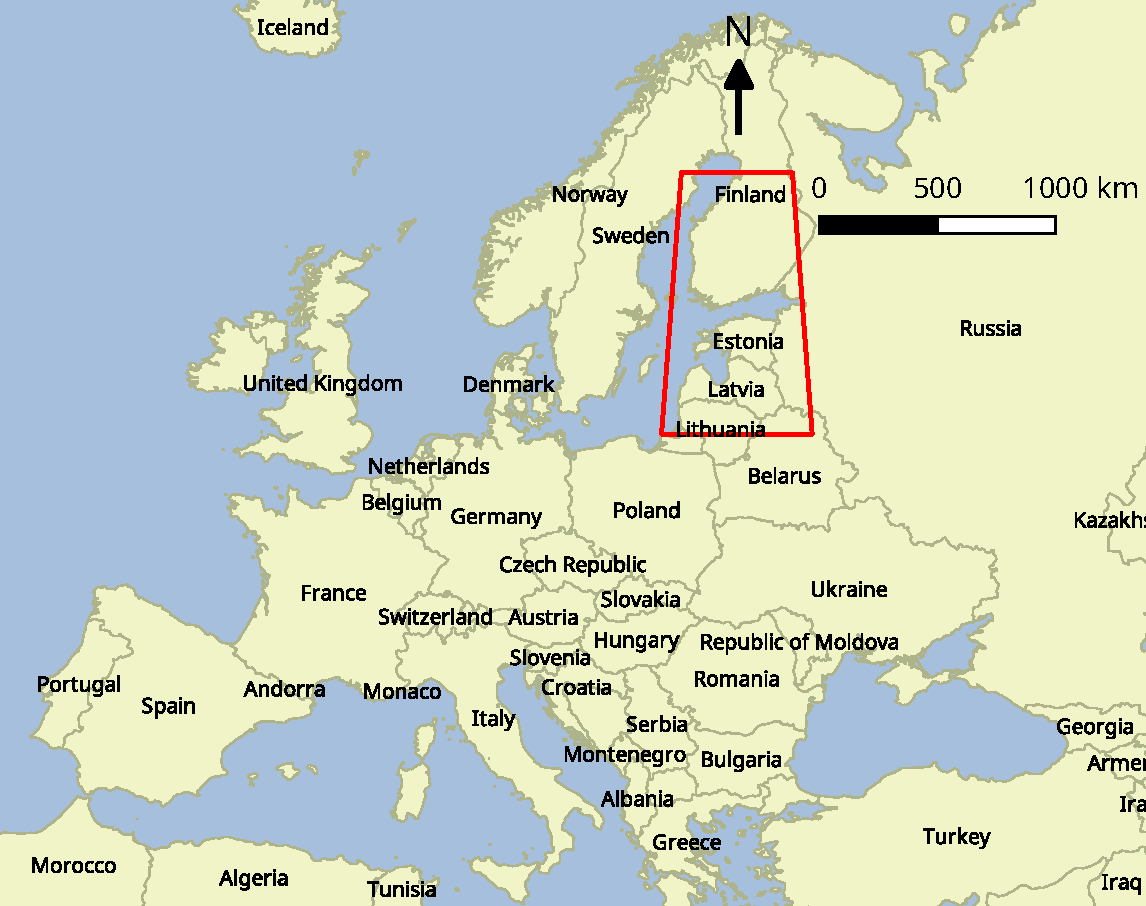
\includegraphics[width=0.6\textwidth]{./thesis-figures/aoi}
 \caption{Study area (PROBA-V tile X20Y01) highlighted in red. Basemap created using the World Borders dataset \citep{worldborders}.}
 \label{AOI}
\end{figure} 

The chosen study area is based on the PROBA-V tile 20,01, which has an extent of 20 to 30 degrees longitude and 55 to 65 degrees latitude. It spans from south Finland, known for boreal forests as well as a variety of lakes and boreal wetlands, to the middle of Lithuania, which includes both mixed and temperate broadleaf forests as well as protected wetlands (see figure \ref{AOI}).

The land cover classes that were used for classification are based on the generalised land cover legend by \citet{see2015hybrid} and \citet{Herold2008lccomparison}, adjusted to fit the study area. Permanent snow and ice was not included due to the study area lacking this class. The distinction between needleleaf and broadleaf tree cover was dropped as well, due to tree stands in the study area being dominated by needleleaf trees in the evergreen category and broadleaf trees in the deciduous category. Thus nine classes were defined as follows:

\begin{enumerate}
 \item \textbf{Cultivated}: human-managed herbaceous vegetation that is harvested at least once per year, including pastures and agricultural crops.
 \item \textbf{Deciduous trees}: woody vegetation taller than 3 metres in height, which drops its foliage during the cold season.
 \item \textbf{Evergreen trees}: woody vegetation taller than 3 metres in height, which retains its foliage all year round.
 \item \textbf{Shrubs}: woody vegetation shorter than 3 metres in height, including young stands of deciduous or evergreen trees.
 \item \textbf{Grass}: well-drained natural herbaceous vegetation.
 \item \textbf{Barren}: soils not covered by vegetation or artificial cover, including sand dunes, beaches, gravel and sand pits (for mining, construction, or natural), gravel and dirt roads, as well as rocky cover such as boulders and rocky cliffsides.
 \item \textbf{Wetland}: waterlogged natural herbaceous vegetation and peat.
 \item \textbf{Built-up}: artificial land cover, including buildings and paved roads.
 \item \textbf{Water}: ground covered by water, both inland and seawater, including water within wetland areas.
\end{enumerate}

\section{Data}

For this study, a variety of data was required, with varying levels of preprocessing needed for each. Some data was derived from other data. Ground truth data was used for training and validating classification algorithm performance, and consisted of 480 points, each containing the fraction of each land cover class within the associated PROBA-V pixel. Covariates are raster data, used by algorithms as data from which to derive the land cover class proportions. When predicting, only covariates are made available to the algorithm, and ground truth is used to validate how well each algorithm performs. Covariate data can also be divided into spectral, temporal, elevation and auxiliary data.

\subsection{Ground truth data}

\subsubsection{Data availability}

In order to make use of supervised classification algorithms, a representative dataset of ground truth at the area of interest has to be obtained for training the algorithms, as well as validating the classification accuracy. When working with fuzzy classification, the ground truth has to be in the same schema as the desired output from the classification algorithms. That means that every ground truth point has to contain information about the proportion of each land cover class within the cell associated with the ground truth point.

No such dataset was available at the time of writing. The closest available was the Geo-Wiki Land Cover Classification Competition II result dataset \citep{perger2012geowiki}. Competition participants identified the proportions of three dominant land cover classes in 300 m pixels. However, this dataset was not suitable for this study, because the study area only had 14 points classified, the contestants rarely agreed about the class proportions and only up to three dominant ones were considered, and the competition was based on coarser resolution data that did not match PROBA-V pixels.

This meant that ground truth had to be collected manually specifically for the purposes of this study. Manual remote sensing image interpretation \citep{defries1998training} was used to achieve this. The target was to obtain at least 50 ground truth pixels for every class. A pixel was considered to belong to a certain class if that class had the majority fraction in the pixel. In addition, at least 15 pixels of each class had to be endmember pixels: ones that amount for 95\% or larger fractions within the pixel. The result was a dataset of 480 ground truth pixels in total.

\subsubsection{Collection methods}

For determining which pixels to sample, a two-stage selection protocol was used. The first stage was stratified random sampling based on the 2010 CCI Land Cover product by the European Space Agency \citep{lccciguide}. Since this product uses a larger number of classes (since it is a hard rather than a fuzzy classification), some classes were merged into one to fit the classes desired in this study. See Appendix \ref{appendix-classes} for more details. 112 pixels per class (total of 1008) were selected in this stage.

The first stage selected pixels that were not always optimal for the needs of this study. First, endmember pixels were needed, while the vast majority of pixels are mixed. Second, the LC-CCI product uses coarser resolution pixels than the PROBA-V data used for classification, therefore the equivalent PROBA-V pixels were not necessarily of the desired land cover class. Third, LC-CCI classification was not always accurate, possibly due to inaccuracies in the classification algorithm used to derive it, and possibly due to land cover changes over time (PROBA-V data goes back only to 2013, three years later than what the LC-CCI product was made for). Fourth, the study requires ground truth where land cover has remained constant over the last three years, whereas in some locations there was clear land cover change occurring (mostly due to deforestation). Therefore a systematic second stage selection was performed for each pixel selected in the first stage. Pixels within a 10 pixel radius from the first stage selection were manually checked, and the best pixel was selected for each. The criteria used, in order, were:

\begin{enumerate}
 \item Evident land cover change: no pixels with identifiable land cover change over the 2013-2016 period were used.
 \item Uncertainty in identification of land cover proportions in the pixel: pixels that had more unambiguous reference layers were preferred in order to minimise the uncertainty in the resulting dataset.
 \item Purity of the pixel: pixels with one highly dominant land cover class were preferred, so that enough endmember pixels could be collected.
 \item Distance from the pixel selected in the first stage: in case all other criteria were equal for several pixels, the pixel closest to the pixel selected in the first stage was chosen.
\end{enumerate}

In case none of the pixels within the 10 pixel radius fulfilled the selection criteria, the area was skipped. In case the LC-CCI classification had mislabelled the area, a pixel of another class than the one desired could also be selected, provided it fulfils the above criteria. For example, the LC-CCI classification often confused urban and barren areas; in those cases, the best pixel was selected and identified appropriately, no matter which class it was labelled as in LC-CCI. See figure \ref{fig-sampling} for an example.

\begin{figure}
 \centering
 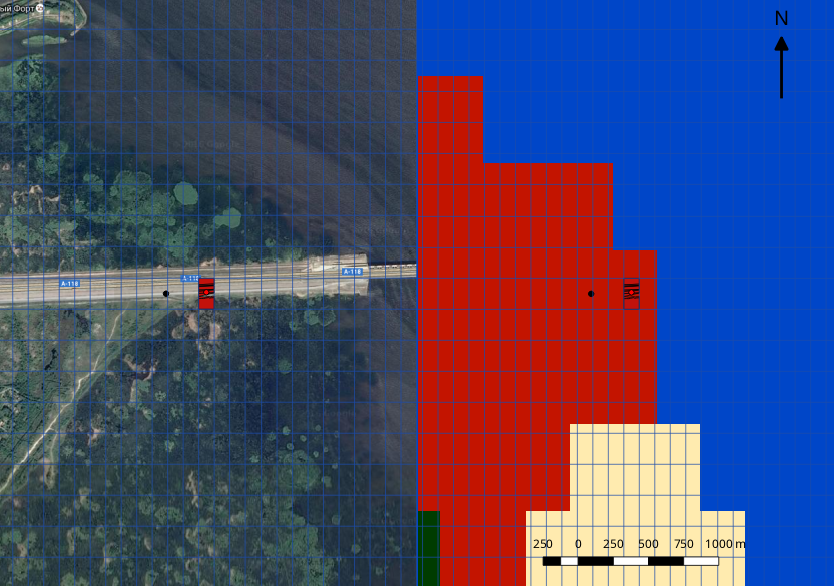
\includegraphics[width=0.8\textwidth]{./thesis-figures/classification-example.png}
 \caption{An example of a ground truth pixel within an area misclassified by LC-CCI. Left: a true colour image of an area on Kotlin island, north of Kronstadt, Russia (Google Maps imagery). Right: LC-CCI classification of the same area. Red: urban areas, cream: sparsely vegetated areas, green: needleleaved evergreen trees. In reality, the area is mainly composed of wetland. The black point represents the first stage sample, the red point represents the second stage sample. The blue grid indicates PROBA-V pixel locations. The polygons around the second stage sample were used for measuring the area of each land cover type within the pixel. The result was 36\% wetland, 28\% built-up, 23\% barren, 8\% grass, 5\% shrubs, 0\% of the rest.}
 \label{fig-sampling}
\end{figure}

Image interpretation, second stage sample selection and dataset creation were performed using QGIS 2.14.8 ``Essen'' software. To aid in visual interpretation in order to ensure that the gathered ground truth would have as little uncertainty as possible, open national data (orthophotos and topographical maps) from Finland, Estonia, Latvia and Lithuania was used in addition to open global data. In addition to GIS layers, panoramic photos were used (Google Street View, Yandex panoramas). For a full list of layers used for image interpretation, see Appendix \ref{app-layerlist}.

In order to determine the class proportions within a PROBA-V pixel, instead of relying on subjective estimations or subdivision, land cover within a pixel was outlined by drawing multipart polygons for each class (except the dominant) on top of the pixel area. Then by using a QGIS virtual attribute, the area of each polygon was dynamically calculated and divided by the total area of a pixel (which is constant among all pixels in the WGS84 coordinate reference system), giving a percentage fraction of each class. The fraction of the dominant class was then calculated by subtracting each of the other fractions from 100\%. Therefore the precision of the ground truth data is 1\%, and the range is from 0\% to 100\%.

Gathered ground truth data was stored as a point layer, with each point representing the PROBA-V pixel footprint under it. In order to make certain that there are no issues with points falling on pixel borders, as well as to accurately know the boundaries of each pixel when drawing polygons on it, a line grid was generated in QGIS by using an imported PROBA-V image as a reference for the origin and size of each grid cell. Ground truth points were placed in the centre of the pixel they describe, and snapping (with topology checking) was used when drawing polygons in order to avoid geometry errors and imprecisions.

The resulting sample points were then exported into a CSV file, which then was imported into R. Each attribute in R is available as a variable, so they can then be used in classification.

\subsubsection{Interpretation protocol}

In order to better discern land cover classes and minimise the uncertainty of land cover proportions in the gathered ground truth dataset, various approaches were used for each land cover class. While these approaches minimise uncertainty, they still do not guarantee error-free interpretation, however. For a summary of the approaches, see table \ref{tbl-protocol}.

\begin{table}
  \centering
  \begin{tabular}{p{0.4\textwidth}p{0.55\textwidth}}
    Image interpretation problem & Approach to minimise uncertainty\\ \hline
    Land cover change & Areas with evident change skipped\\
    Differences in orthorectification & National data preferred\\
    Multiple images covering the same area & Finest spatial resolution or most recent preferred\\
    Seasonal tree canopy change & Estimated summer canopy extent used\\
    Pasture identification and classification & Panoramic images used to look for signs of management; if found, assigned as cultivated, else assigned as grass\\
    Distinction between evergreen and deciduous trees & Autumn/winter images and 3D imagery used where available; panoramic images used to identify the first row of trees, overhead imagery for the rest\\
    Distinction between shrubs and trees & Panoramic images used; shadow comparison at low sun angles\\
    Distinction between gravel and asphalt roads & Panoramic images used\\
    Distinction between wetland and grass & National topographic data used
  \end{tabular}
  \caption{Summary of the approaches used to minimise uncertainty in image interpretation.}
  \label{tbl-protocol}
\end{table}

While a large number of imagery sources were used to determine the land cover, their date of acquisition varies between different sources. Some of the sources, like Bing, do not give information about the year the image was taken. If land cover changes affecting the class proportions were evident from the images, such pixels were not used as ground truth, but there exists a possibility that there had been land cover changes that were not identified due to the lack of recent imagery.

Another source of uncertainty comes from orthorectification of the imagery. Different sources were slightly offset from one another, in particular, Bing aerial imagery tended to be shifted around 16 metres from Google imagery of the same area in some places, and around 9 metres from national orthophoto imagery. When possible, Bing imagery was not used in favour of the other sources for drawing area measurement polygons. From those, the most recent or most detailed image was used.

Similarly, the look angle of the sensors tended to vary between images. That had most impact for tall objects, like tree canopies. Like with the point above, the most recent or finer resolution image was used as the main reference in that case. In addition, for deciduous trees, the season when the image was taken had an effect on the perception of tree canopies. In summer images, the canopy would seem to take up more area of the pixel than in images taken in other seasons. In order to cope with this problem, for images taken in other seasons, the polygons drawn on top of the trees were made larger to compensate, by estimating the area the canopy would take up if it was summer time.

Specifically for the cultivated area class, there was a possibility of confusing it with the grass class for managed pastures. Since pastures are also often managed and hay harvested, and there were not enough images to reliably detect whether at some point in the year the field is indeed harvested, there may be confusion as to which class to assign such a field. To mitigate this problem, panoramic images were used to identify haystacks, fences and cattle in the fields, whose presence would indicate that the field is managed.

The distinction between evergreen and deciduous trees was also challenging. Within the study area, forests and stands primarily include trees of genus \textit{Betula} L. (birch trees), genus \textit{Pinus} L. (pine trees), of whom mostly \textit{Pinus sylvestris} L. (scots pine), and genus \textit{Picea} Mill. (spruce trees), of whom mostly \textit{Picea abies} (L.) H. Karst. (Norway spruce). Spruce canopies are distinctly conical, which allows distinguishing them from birch trees, but not from young pine trees. Also, very fine resolution imagery is required to tell the canopy shape in the first place. Such imagery was mostly available only in Estonia and parts of Finland. Distinguishing between birch trees and pine trees is even more challenging, since their canopy shape is very similar when looking from the top.

Two main approaches were used to deal with this source of uncertainty. The first approach was making use of imagery taken in seasons other than summer. In autumn, leaf senescence allows identifying deciduous trees directly by colour. In winter and spring, deciduous trees are difficult to discern from the forest floor, but by comparison with summer images, they show which areas consist of deciduous trees. In addition, such images reveal all evergreen trees within mixed forests. One pitfall of this approach could be that the changes in apparent tree cover between the images is not due to seasonality, but rather due to deforestation; however in practice, tree trunks are still visible in winter and spring imagery. With this approach, Estonian national imagery was most useful, since it was taken in late autumn and has a fine enough resolution to identify individual trees.

\begin{figure}
  \centering
  \begin{subfigure}[b]{0.7\textwidth}
   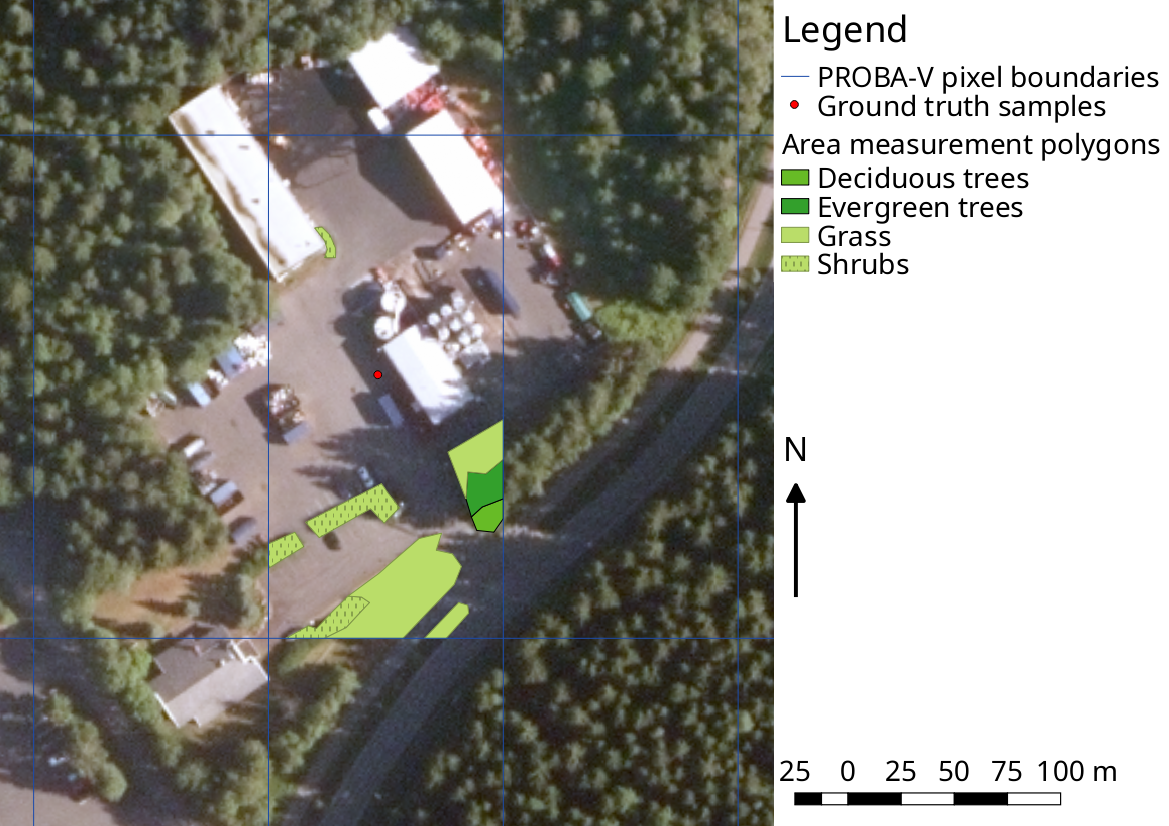
\includegraphics[width=\textwidth]{./thesis-figures/sample-example.png}
   \caption{A sampled area in the town of Jyv\"askyl\"a, Finland.}
  \end{subfigure}
  \begin{subfigure}[b]{0.65\textwidth}
   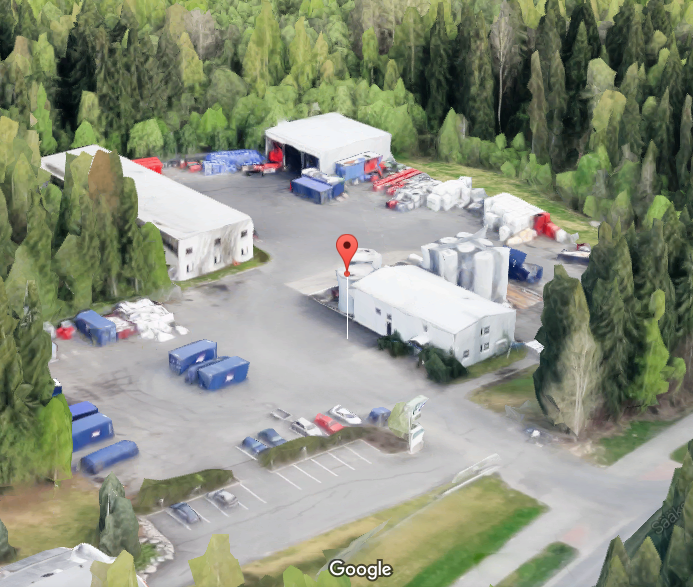
\includegraphics[width=\textwidth]{./thesis-figures/sample-3d.png}
   \caption{The same area in Google Maps, using 3D view.}
  \end{subfigure}
  \caption{A close-up example of a sampled area for which 3D view was available for improved distinction between classes. The resulting land cover fractions were 87\% built-up, 8\% grass, 3\% shrubs, 1\% evergreen trees, 1\% deciduous trees, 0\% others.}
  \label{fig-sampling-detailed}
\end{figure}

The second approach was to make use of auxiliary data. Most helpful were panoramic images, from which tree species could be identified directly. The limitation of this approach is that panoramic images are relatively scarce, limited to areas near roads. Also, typically only the first row of trees is visible in these images. But that is often enough to determine the proportion of deciduous and evergreen trees within a forest, and is useful when combined with remote sensing imagery, since by identifying the first tree row, further trees can be discerned by comparison. Another useful source of information were 3D models provided by Google Maps in certain areas. They are detailed enough to discern individual trees and their canopy shape, which allows identifying their type (see figure \ref{fig-sampling-detailed}). Other auxiliary data used were topographical maps, which sometimes marked forest types, and the LC-CCI classification map. Though this data was often not precise enough for the needs of this study. Lastly, in some images where the sun zenith angle was low, shadows could be used to determine the canopy shape of the first row of trees as well. But it was rather rare for this information to be useful, given the similarity in upper canopy between birch and pine trees.

Shrubs were problematic to distinguish between grass and both types of trees. Since the distinguishing factor for shrubs was height, the shrub class included young trees and hedges, but not low underwood species like \textit{Malus pumila} Mill. (apple trees). However, since most remote sensing imagery used was 2D, determining the height was problematic. One approach to distinguishing shrubs from trees was by comparison with other tree stands in the immediate vicinity. Since for most imagery the look angle was not equal to nadir, or there were shadows visible, comparing them with tree stands allows identification of this class. Another approach was once again to use panoramic photos in order to either identify the type of plants directly, or to estimate the height of the plants. The distinction between tall herbaceous species (grass) and short woody species (shrubs) was also problematic at times. Panoramic photos were used in that case as well. Another consideration for this class is that within the area of interest, shrublands are a transitory ecosystem between grasslands and forests, they do not normally form a climax community. Similarly, young trees are transitory between grasslands (or, in case of reforestation, forest floor) and forests. In order to deal with this temporal aspect, all the available imagery was checked for differences of appearance between the images of different dates. If a patch of plants within a pixel appeared either as grass or as tall trees in any of the images, such a pixel was not used.

While the barren class was mostly easy to distinguish from the other classes, the specific case of roads lead to some uncertainty. Gravel roads were considered as barren cover, while asphalt roads as well as roads made of concrete tiles were considered built-up cover. In some of the imagery, the distinction of colour between the two was difficult to make, particularly in cases of eroded asphalt and asphalt covered by a thin layer of sand or dust. In those cases, panoramic photos were used to make a better distinction. Since there was a wealth of such photos taken on roads, this was for the most part a minor issue.

Wetlands were somewhat challenging to distinguish from grass and shrubs. This is by definition, since within the study area wetlands are covered by herbaceous or short woody vegetation. The distinguishing factor is whether the area is waterlogged or drained. Within the study area most wetlands are large, contiguous, often protected territories, so topographical maps were useful in distinguishing them. In addition, wetlands tend to have a brown tint due to peat, which is more evident when zoomed out. The LC-CCI map turned out to be rather accurate in detecting wetlands, so it was also used for reference.

\subsection{Spectral data}
\label{sec-spectral}

\subsubsection{Data availability}

Spectral data for this study was obtained from the PROBA-V sensor, provided by VITO. The PROBA-V sensor captures 4 spectral bands: blue, red, near infrared and shortwave infrared. In addition, VITO also provides an NDVI product calculated from the aforementioned bands. The data is provided as rasters in the WGS84 coordinate reference system. In this thesis, the 100 m resolution level 3 top-of-canopy reflectance product was used. Despite the name of the product, the cartesian cell size varies depending on the latitude, since cell boundaries are defined by polar coordinates. On average, the cell size at the area of interest is approximately 109 $\times{}$ 221 m, stretched in the north-south direction. Each image of a 10-by-10-degree tile contains 10080 $\times{}$ 10080 pixels (101.6 megapixels) per band. Radiometry bands are stored as 16-bit signed integers, and NDVI is stored as 32-bit floating point units.

This product is available in composites of five days, made by compositing five one-day composites by using maximum NDVI, after filtering out pixels of poor quality, such as incomplete data, sensor problems and extreme sun or look angles. A quality control layer is also provided, with information on whether a pixel is clouded, shadowed, on land or over water, and whether the sensors for each band were working according to specifications at the time of data acquisition \citep{probavguide2}.

The data comes in two collections, which differ in the algorithm used to detect clouds. A known limitation of the cloud detection algorithm used for Collection 0 data made it not sufficient to fully detect all clouds. A reprocessing campaign using a more accurate algorithm that resulted in Collection 1 data \citep{probavguide2} was ongoing at the time of writing, with the oldest images being reprocessed first. At the time of running the algorithms, most data was already processed to Collection 1, with the only gaps being the month of November, 2016 and the single date of June 6, 2016. Collection 0 data was used for those dates.

\subsubsection{Data preprocessing}
\label{sec-spectral-preprocessing}

Spectral data preprocessing involved four major steps: cloud filtering using the built-in quality control layers, cloud filtering by discarding temporal outliers, compositing and deriving indices from the composite. See figure \ref{fig-optical-flowchart} for more details. All preprocessing, algorithm training and prediction was done on a shared virtual machine provided by VITO, which had 32 processor cores (Intel Xeon E3, 2.4 GHz) and 32.8 gigabytes of memory.

\begin{figure}
  \centering
  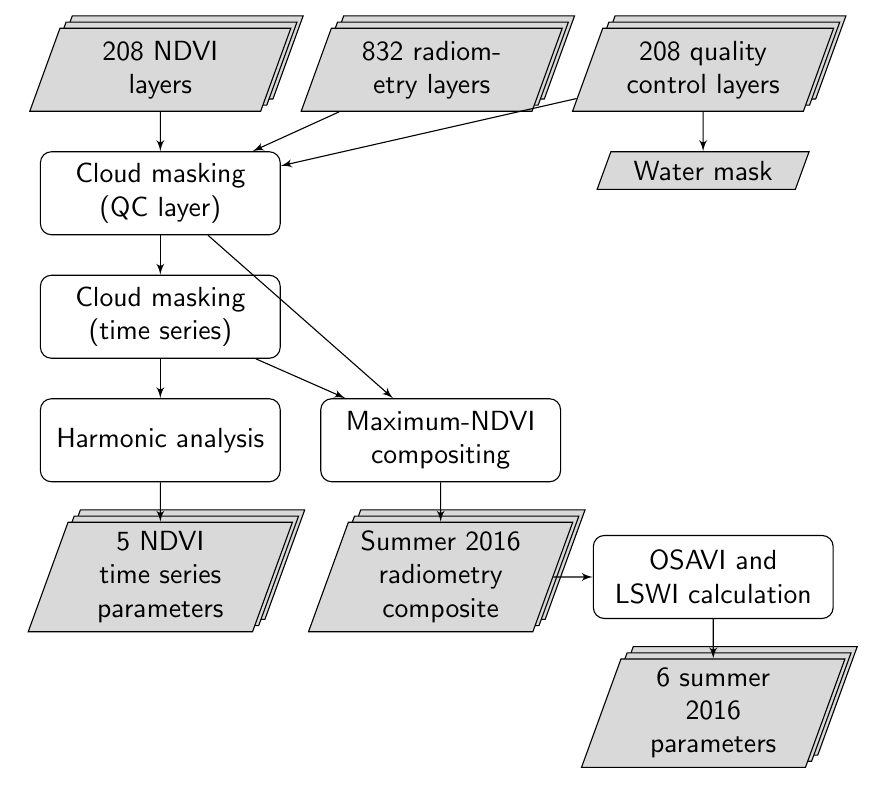
\begin{tikzpicture}[node distance = 0.5cm, auto]
      % Optical
      \node [data] (radiometry) {832 radiometry layers};
      \node [data, left= of radiometry] (ndvi) {208 NDVI layers};
      \node [data, right= of radiometry] (qc) {208 quality control layers};
      \node [block, below= of ndvi] (clean-builtin) {Cloud masking (QC layer)};
      \node [block, below= of clean-builtin] (clean-timeseries) {Cloud masking (time series)};
      \node [block, below= of clean-timeseries] (get-harmonics) {Harmonic analysis};
      \node [block, right= of get-harmonics] (composite-probav) {Maximum-NDVI compositing};
      \node [data, below= of composite-probav] (composite) {Summer 2016 radiometry composite};
      \node [block, right= of composite] (calc-indices) {OSAVI and LSWI calculation};
      \node [data, below= of calc-indices] (indices) {6 summer 2016 parameters};
      \node [data, below= of get-harmonics] (harmonics) {5 NDVI time series parameters};
      \node [datasingle, below= of qc] (iswater) {Water mask};
      % Draw edges
      \path [line] (radiometry) -- (clean-builtin);
      \path [line] (ndvi) -- (clean-builtin);
      \path [line] (qc) -- (clean-builtin);
      \path [line] (clean-builtin) -- (clean-timeseries);
      \path [line] (clean-timeseries) -- (composite-probav);
      \path [line] (clean-builtin) -- (composite-probav);
      \path [line] (composite-probav) -- (composite);
      \path [line] (composite) -- (calc-indices);
      \path [line] (qc) -- (iswater);
      \path [line] (calc-indices) -- (indices);
      \path [line] (clean-timeseries) -- (get-harmonics);
      \path [line] (get-harmonics) -- (harmonics);
  \end{tikzpicture}
  \caption{Flowchart of the spectral and temporal parameter preprocessing chain. Grey blocks are input and output data, white blocks are scripts that process the data. The radiometry layers are a set of 4 spectral bands (blue, red, NIR, SWIR) for each time step; all input layers were 5-day composites for a period of 2014-2016.}
  \label{fig-optical-flowchart}
\end{figure}

The first step in the preprocesing chain was to mask out pixels of bad quality according to the quality control layers provided by VITO. Pixels  that were marked as having clouds, cloud shadows, ice, as well as any pixels reported as bad due to sensor malfunctions, were masked out using the \textit{R} package \textit{probaV} \citep{eberenz2016probav}. A total of 1040 raster layers (208 5-day composites with 4 radiometry bands and one NDVI layer) were filtered of clouds using data from 208 quality control layers. A single NDVI layer took approximately 43 seconds to filter, one set of radiometry (4 bands) took approximately 97 seconds to filter. Cloud filtering was run using 3 threads, so as not to run out of memory, which results in around 50 minute run time for all NDVI layers and 112 minute run time for all radiometry layers.

While Collection 1 improved the cloud detection algorithm, it still does not detect clouds over water well enough, and tends to confuse barren areas with clouds. In addition, cloud shadow detection has become worse, with one-pixel-wide shadows not being masked properly. Due to the problems with cloud masking in the provided data, extra cloud masking was performed by discarding temporal outliers.

Temporal outliers caused by undetected cloud cover were additionally filtered out by fitting a LOESS curve on a time series of remaining blue band observations for each pixel, and marking positive outliers that deviate more than 30 digital numbers (0.015 reflectance values) from the LOESS curve as clouds. This was also done using the \textit{R} package \textit{probaV}. The output of this step is a new cloud mask layer. In order to make use of multithreaded processing, the input raster layers were first stacked into a time series, and then the stack was divided into 1680 blocks, with 30 of them being processed in parallel. Processing took 14 hours, and mosaicking the blocks back into one file using \textit{GDAL} took an extra 33 minutes.

Then the resulting temporal cloud mask was applied to NDVI time series to filter the clouds from it by writing an \textit{R} script that makes use of the \textit{raster}, \textit{foreach} and \textit{doParallel} packages to perform the cloud masking in parallel on 20 threads. This step took 16 minutes.

After applying both cloud masking methods, the resulting rasters had a large amount of no data values. This posed a problem, since several of the classification algorithms used cannot handle data with missing values. In order to solve this problem, a radiometry composite was created from the images of the whole summer of 2016 (2016-06-01 to 2016-08-31, 18 images in total). This period was selected to minimise the effects of snow and leaf senescence \citep{bartalev2014probavboreal}. Compositing was done by selecting pixels using maximum NDVI, in cases where more than one raster layer had values at that location. The NDVI layers used for this were the ones obtained by using temporal cloud masking as outlined above, whereas the radiometry layers used in this step were only masked using the quality control layers. Since maximum NDVI selection precludes no data values, the method selected only cloud-free radiometry. This saved some processing time and disk space that would have been required for applying the temporal cloud mask to each of the radiometry layers.

In addition to spectral data itself, vegetation indices derived from spectral data are known to improve the separability of the wetlands class \citep{zhao2009indices,davranche2010wetland}. However, since the PROBA-V sensor only captures four spectral bands, the choice of available vegetation indices is limited. Therefore two vegetation indices that can be calculated and are known to improve wetlands separability were used: Optimised Soil-Adjusted Vegetation Index (OSAVI, \citealt{rondeaux1996osavi}) and Land Surface Water Index (LSWI, \citealt{xiao2004lswi, dong2014lswi}). These indices were calculated from the 2016 summer composite image. LSWI was calculated by using the formula:

$$ LSWI = \frac{NIR - SWIR}{NIR + SWIR} $$

where $NIR$ is the near infrared band, and $SWIR$ is the shortwave infrared band of PROBA-V. In addition, the Optimised Soil-Adjusted Vegetation Index (OSAVI) was calculated by using the formula:

$$ OSAVI = 1.16 \cdot{} \frac{NIR-RED}{NIR+RED+0.16} $$

where $RED$ is the red band of PROBA-V.

All in all, preprocessing spectral data resulted in 6 parameters to be used as covariates for algorithm training and prediction: reflectance is the red band, reflectance in the blue band, reflectance in the near infrared band, reflectance in the shortwave infrared band, Land Surface Water Index and Optimised Soil-Adjusted Vegetation Index.

\subsection{Temporal data}

PROBA-V imagery was also used for deriving temporal data: vegetation growth phase and amplitude, \nth{1} and \nth{2} order (period of a year and half a year, respectively). NDVI provided by PROBA-V throughout the mission duration (2013-2016, 3 years), after cloud filtering as described in section \ref{sec-spectral-preprocessing}, was used for deriving the temporal data (see figure \ref{fig-optical-flowchart}).

Phase and amplitude metrics were extracted out of the time series by performing harmonic time series analysis \citep{rayner1971introduction,jakubauskas2001harmonic} on it. This was done using \textit{R} in two steps. First, a linear model was fitted to the data (for each pixel):

$$ y(t) = a_1 \sin{(t\cdot{\tau{}})} + b_1 \cos{(t\cdot{\tau{}})} + a_2 \sin{(t\cdot{2\tau{}})} + b_2 \cos{(t\cdot{2\tau{}})} + \epsilon{} $$

where $t$ is time (fraction of a year), $y(t)$ is the NDVI value at time $t$, $a_1$, $b_1$, $a_2$ and $b_2$ are coefficients to be determined (index denotes the order of the harmonic: 1 for a harmonic with a period of a year, 2 for a harmonic with a period of half a year), $\epsilon{}$ is the error term and $\tau{} = 2\pi{}$.

Afterwards, amplitude $A$ was calculated from the coefficients by using the formula:

$$ A_n = \sqrt{a_n + b_n} $$

where $n$ denotes the order of the harmonic. Phase $\phi{}$ was calculated using the formula:

$$ \phi{}_n = \Arctan{(a_n, b_n)} \bmod{\tau{}} $$

The amplitude parameters describe the intensity of change in NDVI over a period of a year and half a year, but they do not contain information about what NDVI value the change fluctuates around. Therefore in addition to the aforementioned parameters, the mean NDVI value for the whole time series was calculated.

All on all, temporal preprocessing of NDVI data resulted in 5 temporal parameters: mean NDVI, \nth{1} order amplitude, \nth{1} order phase, \nth{2} order amplitude and \nth{2} order phase.

NDVI is very popular for deriving time series metrics, since it defines the vegetation growth curve over the course of a year. Any spectral bands or indices derived from them could be used to derive extra time series metrics. In this study only NDVI time series metrics were used, since harmonic analysis yields five parameters per analysed time series, which would greatly increase the total number of covariates. In turn that would require much more processing time and complicate the term selection process for each classification method.

\subsection{Elevation data}

A digital elevation model (DEM) was used to derive elevation, slope, aspect and Topographic Position Index (TPI) terrain parameters. Such terrain parameters are known to increase the separability of vegetation classes \citep{burrough2001fuzzy}.

Initially the DEM from the NASA Global Land Survey (GLSDEM) was considered as the main elevation data source, since it has fine enough spatial resolution (3 arcseconds, approximately 90 m) and is already used by VITO for PROBA-V image ortho-rectification \citep{probavguide}. It is available from the NASA Global Land Survey in 1-by-1 degree tiles. However, this DEM is actually a mosaic of several DEMs, and in the study area above 60\textdegree{} latitude the DEM is based on GTOPO30 data that has 10 times coarser resolution (30 arcseconds, approximately a kilometre), resampled by using cubic convolution to match SRTM data used in the lower latitudes. \citep{glsdemtechguide}. The coarser resolution combined with resampling makes GTOPO30 data unsuitable for deriving slopes, since cubic convolution results in smoothed surfaces, whereas the original GTOPO30 data is of too coarse resolution compared to PROBA-V data. Therefore GLSDEM was only used as an additional data source.

The primary data source was chosen to be the Digital Elevation Model over Europe (EU-DEM) by the European Environment Agency. It has 1-5 arcsecond (approx. 30-150 m) spatial resolution, achieved by fusing data from ASTER and SRTM missions, and covers all of the European Union countries \citep{bashfield2011eudem}. The data is freely available from the European Environment Agency website and is distributed in tiles of 5-by-5 degrees. However, the study area includes not only members of the European Union, but also parts of Belarus and a small part of Russia. As such, GLSDEM was used to fill in the gaps there. See figure \ref{fig-elevation-preprocessing} for the preprocessing chain applied to the elevation data.

\begin{figure}
  \centering
  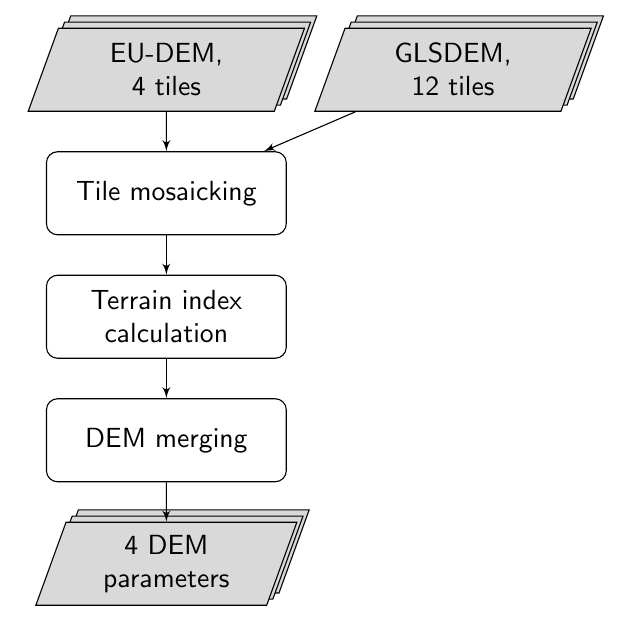
\begin{tikzpicture}[node distance = 0.5cm, auto]
      % DEM
      \node [data] (glsdem) {GLSDEM, 12 tiles};
      \node [data, left= of glsdem] (eudem) {EU-DEM, 4 tiles};
      \node [block, below= of eudem] (mosaic) {Tile mosaicking};
      \node [block, below= of mosaic] (process-eudem) {Terrain index calculation};
      \node [block, below=of process-eudem] (dem-merge) {DEM merging};
      \node [data, below=of dem-merge] (dem-indices) {4 DEM parameters};
      % Draw edges
      \path [line] (glsdem) -- (mosaic);
      \path [line] (eudem) -- (mosaic);
      \path [line] (mosaic) -- (process-eudem);
      \path [line] (process-eudem) -- (dem-merge);
      \path [line] (dem-merge) -- (dem-indices);
  \end{tikzpicture}
  \caption{Elevation parameter preprocessing chain. Grey blocks are input and output data, white blocks are scripts that process the data.}
  \label{fig-elevation-preprocessing}
\end{figure}

Slope was first calculated from the base DEM, using its native resolution and a 4-neighbour moving window (rook's case), since the study area is mostly flat \citep{jones1998dem}. Afterwards, the values were resampled to match PROBA-V pixels. This procedure results in more accurate representation of slopes compared to calculating them from resampled DEM data \citep{grohmann2015demresampling, wu2008demresampling}. Aspect was calculated from a resampled DEM instead, since it is angular data for which regular bilinear interpolation resampling technique does not apply. TPI, which is the difference between the elevation of a cell and the mean elevation of its 8 neighbours \citep{weiss2001topographic, wilson2007terrain}, was also calculated from resampled data due to stark differences in TPI between EU-DEM and GLSDEM datasets, which come from differences in spatial resolution (moving window size).

Next, the two DEMs were merged into one, preferring pixels provided by EU-DEM. For the slope, aspect and TPI statistics, since a moving window was used that created a two-pixel-wide gap of no data around the borders, another moving window filter was applied to interpolate the values from nearest neighbours where data was missing. The moving window matrix was weighted so that the nearest neighbours (in cartesian coordinates) had the most weight, and none of the interpolated values were in locations where ground truth data was collected.

The output of the data preprocessing step is four parameters: elevation, slope, slope aspect and terrain position index (TPI).

\subsection{Auxiliary data}

In addition to the parameters mentioned above, a water mask was extracted from the PROBA-V quality control layers (see figure \ref{fig-optical-flowchart}). This mask holds logical information on whether a particular pixel is covered by water or not, however, it is not completely accurate since it is conservative (shores are marked as land, small islands are marked as water) and does not include inland water bodies.

\section{Classification methods}

Four classification methods have been tested in total: fuzzy \textit{c}-means, fuzzy neural network, random forest regression and multiclass gradient boosting. These methods were chosen due to them being based on very different approaches to the same problem of fuzzy classification, their ability to input and output fuzzy data rather than hard classes, and their implementation availability as packages for the \textit{R} programming language. See table \ref{tbl-comparison} for a short comparison of the properties of the chosen algorithms. Linear mixture modelling was considered, but not included due to covariates other than spectral ones not mixing linearly. Binary relevance method can be used for any regression algorithm; random forest was chosen because it is a very popular method in fuzzy classification, and is related to other decision tree (CART) methods.

\begin{table}
  \begin{center}
    \resizebox{\textwidth}{!}{
      \begin{tabular}{lllll}
	\hline
	Method name & Trains on mixed pixels & Multiple inputs/outputs & Based on\\
	\hline
	Fuzzy \textit{c}-means & Yes & Yes & Feature space statistics\\
	Fuzzy neural network & Yes & Yes & Node weights\\
	Random forest regression & Yes & No & Decision trees\\
	Multiclass gradient boosting & No & Yes & Decision trees\\
	\hline
      \end{tabular}
    }
  \end{center}
  \caption{Feature comparison between the chosen fuzzy classification methods in this study.}
  \label{tbl-comparison}
\end{table}

The tested algorithms were trained on a subset of ground truth data (360 pixels) including the values of the 16 covariates at the pixel locations. Then a prediction was made for the whole PROBA-V tile of the area of interest by providing the algorithms only the covariates. Next, the model was validated by using the remaining ground truth pixels. The process was repeated four times (4-fold cross-validation). See figure \ref{fig-classification-flowchart} for a flowchart representation of the methodology. Lastly, visual validation of the resulting land cover class proportion rasters was performed by training each of the algorithms on all of the ground truth data, and using the resulting models to predict the land cover of the whole PROBA-V tile.

\begin{figure}
  \centering
  \resizebox{\textwidth}{!}{
    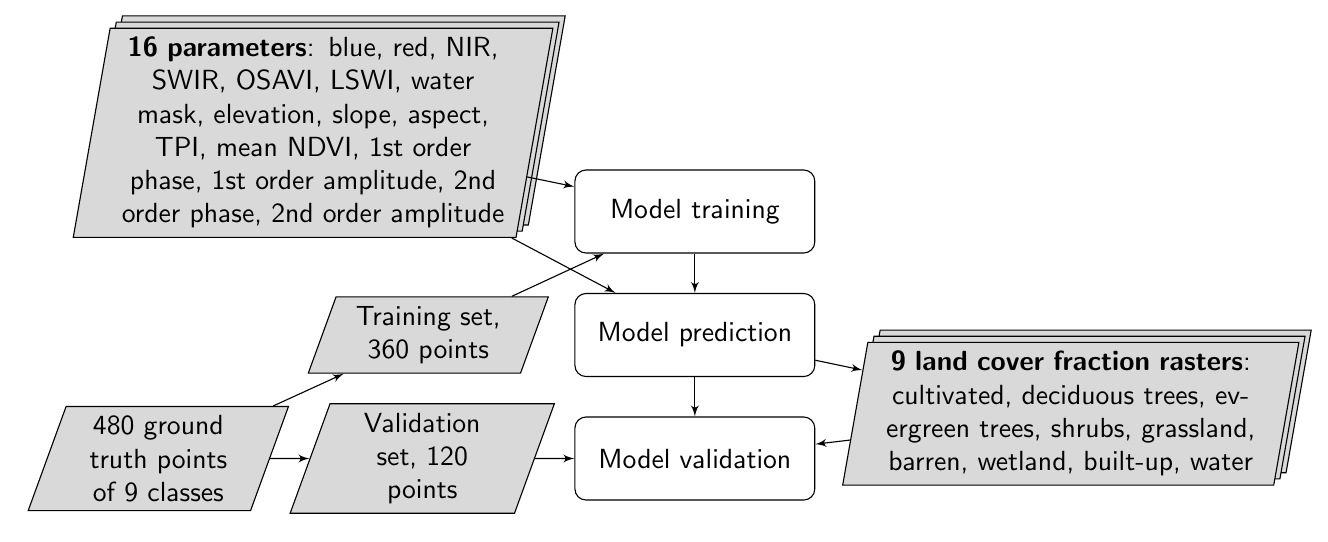
\begin{tikzpicture}[node distance = 0.5cm, auto]
      % Model
      \node [bigdata] (params) {\textbf{16 parameters}: blue, red, NIR, SWIR, OSAVI, LSWI, water mask, elevation, slope, aspect, TPI, mean NDVI, 1st order phase, 1st order amplitude, 2nd order phase, 2nd order amplitude};
      \node [block, right=of params, yshift=-1cm] (training) {Model training};
      \node [block, below=of training] (prediction) {Model prediction};
      \node [block, below=of prediction] (validation-process) {Model validation};
      \node [datasingle, left=of prediction] (training-set) {Training set, 360 points};
      \node [datasingle, left=of validation-process] (validation-set) {Validation set, 120 points};
      \node [datasingle, left=of validation-set] (validation) {480 ground truth points of 9 classes};
      \node [bigdata, right=of prediction, yshift=-1cm] (output) {\textbf{9 land cover fraction rasters}: cultivated, deciduous trees, evergreen trees, shrubs, grassland, barren, wetland, built-up, water};
      % Draw edges
      \path [line] (params) -- (training);
      \path [line] (validation) -- (training-set);
      \path [line] (params) -- (prediction);
      \path [line] (training) -- (prediction);
      \path [line] (prediction) -- (output);
      \path [line] (validation) -- (validation-set);
      \path [line] (prediction) -- (validation-process);
      \path [line] (output) -- (validation-process);
      \path [line] (training-set) -- (training);
      \path [line] (validation-set) -- (validation-process);
    \end{tikzpicture}
  }
  \caption{Generalised classification method training, prediction and validation process. The splitting into training and validation set is automated as 4-fold cross-validation for all methods except multiclass gradient boosting, in which case the training set was all endmember pixels (242) and validation set was all mixed pixels (238).}
  \label{fig-classification-flowchart}
\end{figure}

\subsection{Fuzzy \textit{c}-means}

Fuzzy \textit{c}-means, also called fuzzy \textit{k}-means and supervised fuzzy \textit{k}-means, is a statistical algorithm based on the \textit{k}-means clustering algorithm that attempts to classify pixels by identifying clusters by proximity in feature space. Regular \textit{k}-means is an unsupervised algorithm, and takes one parameter, \textit{k}, for the number of clusters to create. These cluster centroids are usually selected randomly from all pixels, and clusters are formed by assigning each pixel to the class whose centroid is the closest. Then the cluster centroids are recalculated, and the process is repeated until it converges. The supervised variety of this algorithm fixes the cluster centroids to their known values from the training pixels, and the \textit{c}-means or fuzzy \textit{k}-means variety uses the Mahalanobis distance between a given pixel and each class centroid as a measure of class membership \citep{hengl2004fuzzycmeans}. It also takes an extra parameter, called a fuzzy (weighting) exponent (or less commonly a smooth factor or fuzzification parameter), to determine how strongly the distance from the class centroid influences the class membership value. A fuzzy exponent of 1 would result in hard classification, whereas an infinitely high value would result in every pixel belonging to all classes equally regardless of the distance to class centroids \citep{Okeke2006fuzzyexponent}.

The advantage of this algorithm is its simplicity: increasing the number of pixels does not result in high increase in processing time, as only the points' centroid and the distance from each class centroid to each pixel has to be calculated. It is also fuzzy by default, and the prediction results of this method are in the 0-100\% range for each class without the need of postprocessing. The disadvantage of this method is that very little data from the training pixels are used: only the class centroid position and its standard deviation.

This algorithm is implemented as the function \texttt{spfkm} in the \textit{R} package \textit{GSIF}, created by \textit{ISRIC - World Soil Information}. One peculiarity of the \texttt{spfkm} function is that unlike most classification algorithm implementations, it does not have split training and predicting steps, but rather combines both into one. Another peculiarity of this implementation is that it currently requires a \texttt{SpatialPixelsDataFrame} object for the prediction, rather than the more common and memory-safe \texttt{Raster} object.

The \texttt{spfkm} function by default performs a multinomial logistic regression on the training data in order to determine the class centroids. However, multinomial logistic regression can only handle endmember pixels. The \texttt{spfkm} function also allows manually defining class centroid locations and standard deviations. Therefore in order to make use of all pixels, the class centroids and their standard deviation were determined by performing a weighted mean on all pixels for each of the covariates.

In addition, terms and the fuzzy exponent were optimised by repeating the process and selecting the outcomes with the lowest RMSE scores.  First, the optimal fuzzy exponent was determined by calculating RMSE values for the fuzzy exponent range of 1.0-20.0 with an increment of 0.1 (like in \citet{Okeke2006fuzzyexponent}). This was determined to be 1.5. Then, using the optimal fuzzy exponent, terms were dropped one by one until RMSE no longer decreased by dropping more terms. 7 terms were dropped that way, and in addition the water mask was dropped as the algorithm cannot handle binary values. The remaining covariates in the optimal model were near infrared, OSAVI, mean NDVI, elevation, slope and phases of orders 1 and 2.

\subsection{Fuzzy neural network}

Neural networks are a machine learning algorithm that works by making use of a layered architecture of an input layer, output layer, and a number of hidden layers in between. When training, the algorithm tries to assign weights to each node in the hidden layers so that given the input layer, applying the hidden node weights would result in values that match those in the output layer. Initially values are assigned at random, and by using a back-propagation algorithm they are adjusted to better fit the output. Such a trained neural network can then predict the output layer values when given unclassified pixels as the input layer \citep{foody1997fuzzynnet}. Neural networks are implemented in \textit{R} in the package \textit{neuralnet}.

Neural networks work with continuous values, therefore they can take mixed pixels as training input, and output continuous membership values for every class, which makes them well-suited for fuzzy classification tasks. However, there are some downsides of neural networks. One is that they require three parameters: the number of hidden layers, the number of neurons (nodes) per each hidden layer, and the number of back-propagation iterations. Each of these affect the ability of the neural network to generalise data instead of overfitting the training output. Another limitation of neural networks is that they are difficult to train, especially when the training data is not normally distributed and has different ranges for the different covariates. In order to improve training times and prediction results, all the covariates were scaled to the values 0-1 based on the minimum and maximum value of each covariate in the whole ground truth dataset. Lastly, the output of a neural network is not necessarily bound to the range of training data. Thus the predictions require postprocessing so that negative fractions or fractions over 100\% would be eliminated.

This postprocessing can also be done in two ways. The first method is to truncate the output, so that negative values are set to 0 and values over 100\% are set to 100\%, leaving the values in between as-is. The second method is to scale the output range to the 0-100\% range. Scaling the values resulted in lower RMSE values, so this method was used throughout the study.

In the optimisation step, like in the case of fuzzy \textit{c}-means, term selection was performed by dropping terms one by one until RMSE no longer decreased. This resulted in 7 terms being dropped: blue spectral band, OSAVI, aspect, TPI, amplitudes of both orders and the water mask. The number of hidden layers was kept as 1, as a larger number of hidden layers increases the difficulty of training such a model, and the number of nodes in the hidden layer was kept as the mean of the input and output nodes, round down (11 in the unoptimised case, 9 in the optimised case). 10 repetitions (random initial values of the neural network) were used for each model.

\subsection{Random forest regression}

Random forest is a machine learning algorithm based on building decision trees that could be used to determine the class of a pixel. The algorithm generates a (configurably) large number of decision trees, each based on a random (with replacement) training subsample, so that every tree in the model is unique. Then in order to determine which class a pixel belongs to, each decision tree is run and its output counts as a vote. With hard classification, the pixel is assigned the class with the majority vote \citep{walton2008subpixelrf}.

Random forest classification is hard by default, however. There are two main methods for using such algorithms for fuzzy classification tasks. The first option is to use multiclass probabilities. Instead of classifying a pixel using the majority vote, the fraction of votes can be used as an indication of class membership instead. However, the algorithm will have to be trained on endmember pixels only in that case. The second option is to use a binary relevance method. Random forest is capable of performing regressions as well, but only with a single output variable instead of one variable per class. Thus by performing one random forest regression for each class, mixed pixels could be used for training, but the algorithm will not be able to make use of the information about the proportion of other classes in the pixel to be classified.

In this study, the latter method (random forest regression using binary relevance) was chosen, and the former method for the related gradient boosting method (see the next section). The output layers of random forest regression were postprocessed using scaling so that all fractions in each pixel would add up to 100\%.

Random forest is implemented in \textit{R} by several packages. The one used in this study was the \textit{ranger} package, version 0.6.0, as it is implemented in \textit{C++} with faster processing speed and built-in multithreading compared to other packages. It also automates determining covariate importance.

Just like with the algorithms mentioned in the previous sections, an optimisation pass was done for random forest regression as well. Term selection lead to dropping four covariates: OSAVI, elevation, aspect and the water mask. Next, model parameter tweaking was performed. The splitting rule that gave the lowest RMSE values was \textit{maxstat} with a significance threshold \textit{alpha} of 0.9 and lower quantile of covariate distribution \textit{minprop} set to 0.11. For reference, the \textit{ranger} package default values are splitting rule of \textit{variance}, \textit{alpha} of 0.5 and \textit{minprop} of 0.1. The same optimised parameters were applied to all of the models in the binary relevance method, without adjusting them for each class.

\subsection{Multiclass gradient boosting}

Gradient boosting is a machine learning algorithm highly related to random forest. The difference is that instead of building random trees and having them cast votes, the algorithm iteratively optimises a tree (or a small set of trees) to better fit the training data, while making sure not to add unnecessary complexity to the model by performing internal cross-validation at each step. Much like the two aforementioned machine learning methods, it internally uses continuous values, and the result can be expressed as a sum of all tree branch weights \citep{friedman2001gradientboost}. The gradient boosting algorithm is implemented in \textit{R} by the package \textit{xgboost}.

Just like with random forest, there are two ways to use this algorithm for fuzzy classification: the binary relevance method, or a multiclass method that gives the probability of a pixel to belong to each class, akin to the random forest vote proportion method. The same advantages and disadvantages apply. In this study, the multiclass probability method was used in order for the methods to be more differentiated between one another.

Since this method can only be trained on endmember pixels, it was trained on all pixels whose dominant class occupied 95\% of the area or more (242 pixels) and validated by using all mixed pixels (238). However, this makes the error values obtained from this method not directly comparable with ones obtained from the other methods that used 4-fold cross-validation instead.

An optimisation step was also performed for multiclass gradient boosting, however, since the validation set for which the RMSE was counted consisted of only mixed pixels, the optimisation resulted mostly in a strong preference for increased fuzziness. Thus the optimal number of training rounds was set to only 5 (50 in the unoptimised case) and SWIR, OSAVI, LSWI, elevation, aspect and the water mask were dropped in the optimised case.

\section{Validation and visualisation}

\subsection{Statistical validation}

In order to perform validation on the classification results, validation metrics that work on fuzzy classification are needed. While there are several approaches, the metrics that are easiest to interpret and that are most often used for this purpose are based on the well-known statistical concept of error (also referred to as distance in some literature) \citep{foody1996fuzzyevaluation}. In particular, the mean absolute error (MAE) and root mean square error (RMSE) for every class have been used to assess classification accuracy in this thesis. The validation was performed by splitting the ground truth samples into a training and a validation set. For methods that can handle mixed pixel training data, 4-fold cross-validation was used to split the data. For methods that cannot (multiclass gradient boosting), all endmember pixels were used as the training set and all mixed pixels were used as the validation set. The training set was used for training the classification models, and the validation set was used to determine the accuracy of the land cover predictions by:

$$ RMSE_c = \sqrt{ \frac{\displaystyle\sum_{i=1}^{n}{ (p_{i} - v_{i})^2 }}{n} } $$

where $ RMSE_c $ is the root mean squared error of class $ c $, $ v_{i} $ is the true degree of $ i $th pixel's membership to class $ c $ (in percent), $ p_i $ is the predicted degree of $ i $th pixel's membership to class $ c $, and $ n $ is the total number of pixels in an image, and

$$ MAE_c = \frac{\displaystyle\sum_{i=1}^{n}{ |p_{i} - v_{i}| }}{n} $$

where $ MAE_c $ is the mean absolute error of class $ c $.

These two statistics show how many percent did the classification method either overrepresent or underrepresent class $ c $ membership of all pixels in the image on average. The difference between the two is that RMSE gives a larger penalty for large errors compared to MAE.

These statistics allow comparing how well is each classification method capable of predicting the proportion of a given land cover class, much like the diagonal of a confusion matrix does in hard classification. A difference is that this approach does not give information about which land cover classes are confused for which other classes, since misclassification is not binary but rather a matter of degree in fuzzy classification. An overall classification accuracy statistic was obtained by applying the aforementioned formulas to all pixels of the validation set regardless of class.

In addition to accuracy statistics, a bias statistic mean error (ME) was calculated for each class as well:

$$ ME_c = \frac{\displaystyle\sum_{i=1}^{n}{ (p_{i} - v_{i}) }}{n} $$

Positive ME values mean that the classification method tends to overrepresent class $c$ membership, negative ME values mean that it tends to underrepresent class $c$ membership on average in all pixels. An ME of 0 would mean that the classification method is unbiased.

In order to determine whether any method had a significantly lower prediction error than others, a one-way ANOVA test was run on the absolute error values of each pixel for each fuzzy classification method, also including prediction errors of a control method which would always predict equal proportions of each class in every pixel (100\% divided by 9, thereby minimising large errors and hence RMSE). Afterwards, a post-hoc Tukey's range test \citep{tukey1949hsd} was run to determine in pairs which classification methods had significantly lower prediction error than others. 

\subsection{Visual validation}

While error statistics are useful as an objective summary metric of prediction accuracy, they can only be drawn from the validation set, whose size is very small compared to the total number of pixels in a tile (480 pixels out of 101.6 million). Therefore visual validation was performed in addition to statistical validation. First, each of the classification methods were used to predict the land cover proportions in each pixel of the whole study area (PROBA-V tile). Then the prediction accuracy was assessed by comparing prediction results with each other as well as with fine resolution imagery from Google. Comparisons were done by looking at three land cover classes at a time, which could be mapped into the red, green and blue colour channels. The range of colour values was set to be stretched from 0-100 (land cover proportion in percent) to 0-255 in order to better see the differences in proportions. The comparison was done in QGIS, with all the aforementioned data layers overlaid on top of one another for ease of comparison.

\subsection{Covariate importance}

Covariate importance was assessed using permutation importance on holdout random forest regression, as per \citet{Janitza2016holdoutrf}. The holdout technique trains a set of decision trees only on half of the training set supplied to it, and then uses the other half for validation, thus achieving more realistic variable importance metrics compared to using out-of-bag samples for it. Permutation variable importance works by measuring RMSE for a full model, then shuffling the values of the covariate being tested, and tracking the resulting change in RMSE. Most often RMSE increases when values are shuffled, but if a covariate is confounding for a given class, it may decrease and thus the importance reported is negative. Since the covariates have different value ranges, the permutation errors were scaled by the standard error of the training set so as to be comparable with one another \citep{breiman2001random}. Since it is known that permutation importance is biased against correlated covariates \citep{tolosi2011importancebias}, highly correlated covariates were excluded by leaving only the covariate with higher importance in the model. In this study OSAVI and mean NDVI were highly correlated (0.94), and thus OSAVI was excluded.

\chapter{Results}

\section{Classification method accuracy}

\subsection{Statistical comparison}

\subsubsection{Overall errors}

\begin{figure}
  \centering
  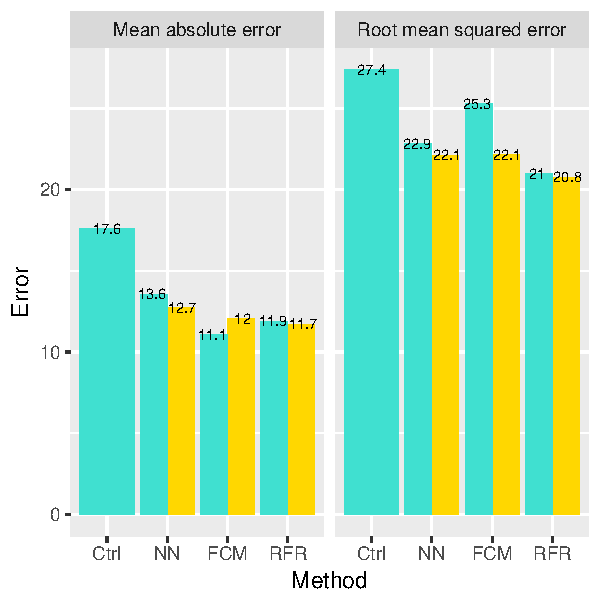
\includegraphics[width=0.55\textwidth]{thesis-figures/total-errors}
  \caption{Overall errors per classification method using 4-fold cross-validation, unoptimised methods (all terms used) in cyan, optimised in yellow. Ctrl: fully fuzzy set (100\%/9 predicted in each cell), NN: neural networks, FCM: fuzzy \textit{c}-means, RFR: random forest regression.}
  \label{fig-total-errors}
\end{figure}

The overall error (errors of all classes combined) of each method except multiclass gradient boosting are shown in figure \ref{fig-total-errors}. The largest difference in RMSE between optimised methods is only 1.3 (6\% difference), thus after optimisations all of the methods exhibit similar prediction accuracy. Likewise, the largest difference in MAE is only 1.0 (8\% difference). Thus while random forest regression achieves the highest prediction accuracy, the difference between the classification methods is very small. The difference in MAE between all the optimised methods (including control) is significant (one-way ANOVA, $p<0.001$). Post-hoc Tukey's range test indicates that all the methods perform significantly better than the control ($p<0.001$) but the differences between the non-control methods are not significant ($p>0.05$), with the difference between neural networks and random forest regression being on the edge of significance ($p=0.06$). Optimising the model by dropping terms and adjusting the fuzziness of the resulting prediction affects fuzzy \textit{c}-means prediction the most (decrease in RMSE of 3.9, which is 13\%), and random forest regression prediction the least (decrease in RMSE of 0.2, which is 1\%).

Multiclass gradient boosting errors are not directly comparable with the errors of other classification methods, as the validation sample size is different, and all validation samples are mixed pixels. So in order to compare multiclass gradient boosting, all methods were also tested by training them on endmember pixels and validating on mixed pixels (see figure \ref{fig-total-errors-gb}). In this case, the control algorithm of assigning each pixel equal land cover class proportions (the 100\%/9 fraction value for each class) has lower errors than in the 4-fold cross-validation scenario above, since a completely fuzzy set is closer to mixed pixels compared to both mixed and endmember pixels. Thus optimising multiclass gradient boosting for lower RMSE in this test increases the fuzziness of the result by decreasing the number of optimisation rounds to just 5. As the number of optimisation rounds increases, the decision trees generated by multiclass gradient boosting are fitted more closely to predict the endmember pixels the model is trained on, and that results in poorer accuracy when trying to predict mixed pixels instead.

\begin{figure}
  \centering
  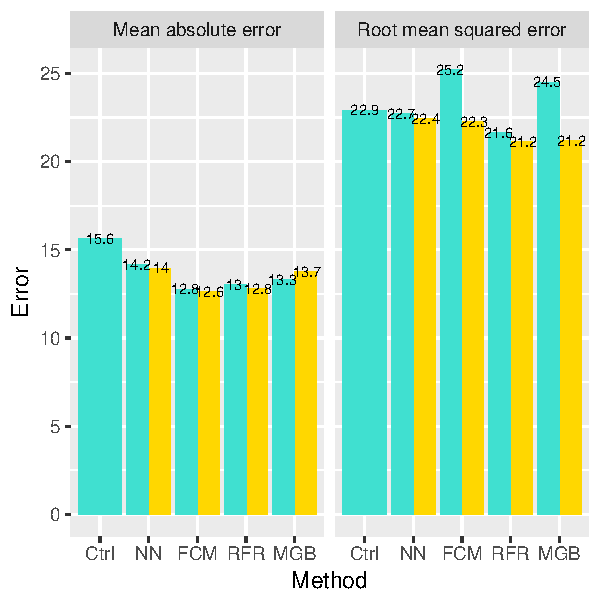
\includegraphics[width=0.55\textwidth]{thesis-figures/total-errors-gb}
  \caption{Overall errors per classification method using holdout validation (training on endmember pixels and validating on mixed pixels), unoptimised methods (all terms used in the model) in cyan, optimised in yellow. Ctrl: fully fuzzy set (100\%/9 predicted in each cell), NN: neural networks, FCM: fuzzy \textit{c}-means, RFR: random forest regression, MGB: multiclass gradient boosting.}
  \label{fig-total-errors-gb}
\end{figure}

The overall mean error (ME) for all classification methods is 0, if rounding errors and floating point imprecision is disregarded. This is an indication that all the resulting predicted class fractions sum up to 100\% for each pixel in all of the classification methods, as the positive errors cancel out the negative errors. ME is more useful for indicating bias per class, however (see the next section).

\subsubsection{Errors per class}

\begin{figure}
  \centering
  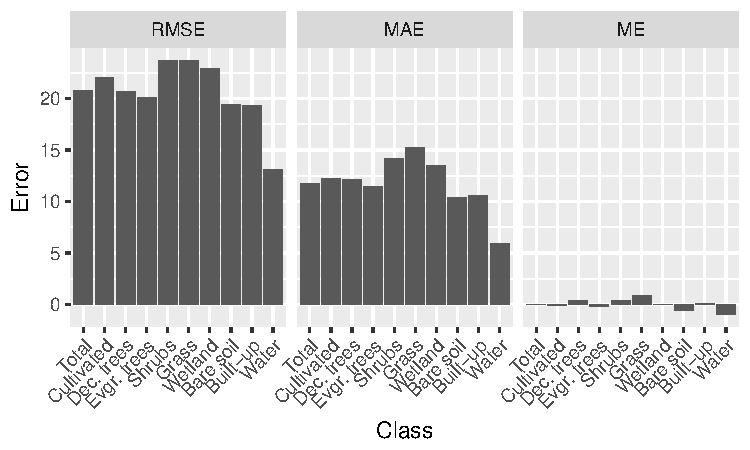
\includegraphics[width=0.8\textwidth]{thesis-figures/perclass-errors-rf}
  \caption{Errors per class using random forest regression. RMSE: root mean squared error, MAE: mean absolute error, ME: mean error.}
  \label{fig-perclass-errors-rf}
\end{figure}

\begin{figure}
  \centering
  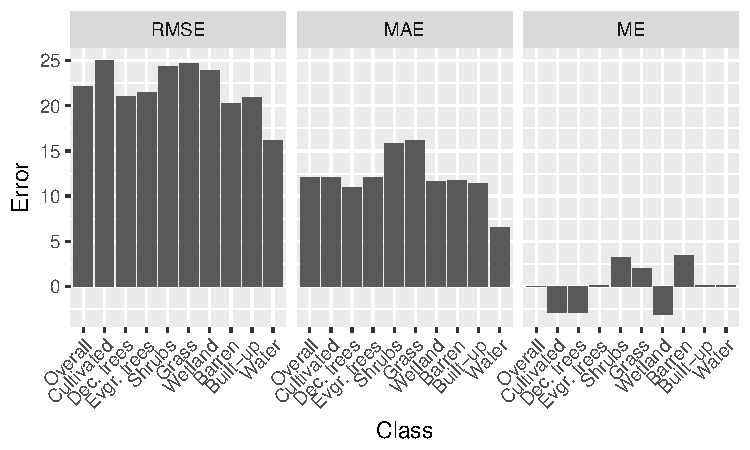
\includegraphics[width=0.8\textwidth]{thesis-figures/perclass-errors-cm}
  \caption{Errors per class using fuzzy \textit{c}-means. RMSE: root mean squared error, MAE: mean absolute error, ME: mean error.}
  \label{fig-perclass-errors-cm}
\end{figure}

When looking at the errors per class for random forest regression (see figure \ref{fig-perclass-errors-rf}), the lowest errors are for the water class. That means it is the easiest to predict the proportion of water in a pixel given the input parameters. Water has several unique properties that makes it easier to discern it from other classes, and many of the water pixels are endmembers due to large bodies of water (sea and lakes) in the area of interest. The classes that were the hardest to predict for random forest regression were shrubs, grass and wetland. Random forest regression tended to slightly overestimate grass and underestimate water proportions in pixels.

Errors per class for fuzzy \textit{c}-means (see figure \ref{fig-perclass-errors-cm}) are similar to ones in random forest regression. The RMSE of the water class prediction of fuzzy \textit{c}-means was larger compared to random forest regression. The most difficult to discern classes for fuzzy \textit{c}-means were shrubs and grass. According to the mean error statistics, fuzzy \textit{c}-means turned out to be much more biased compared to random forest regression, underestimating the proportion of cultivated area, deciduous trees and wetlands while overestimating barren, shrub and grass cover.

Neural network prediction accuracy per class was in between the two classification methods mentioned, with higher mean errors than random forest regression but lower than fuzzy \textit{c}-means (see figure \ref{fig-perclass-errors-nn}). Neural networks tended to particularly underestimate the proportion of water. Just like with the other classification methods, it was easiest to discern water and hardest to discern grass and shrubs.

\subsection{Visual comparison}

\begin{sidewaysfigure}
  \centering
  \begin{subfigure}[t]{.24\textwidth}
    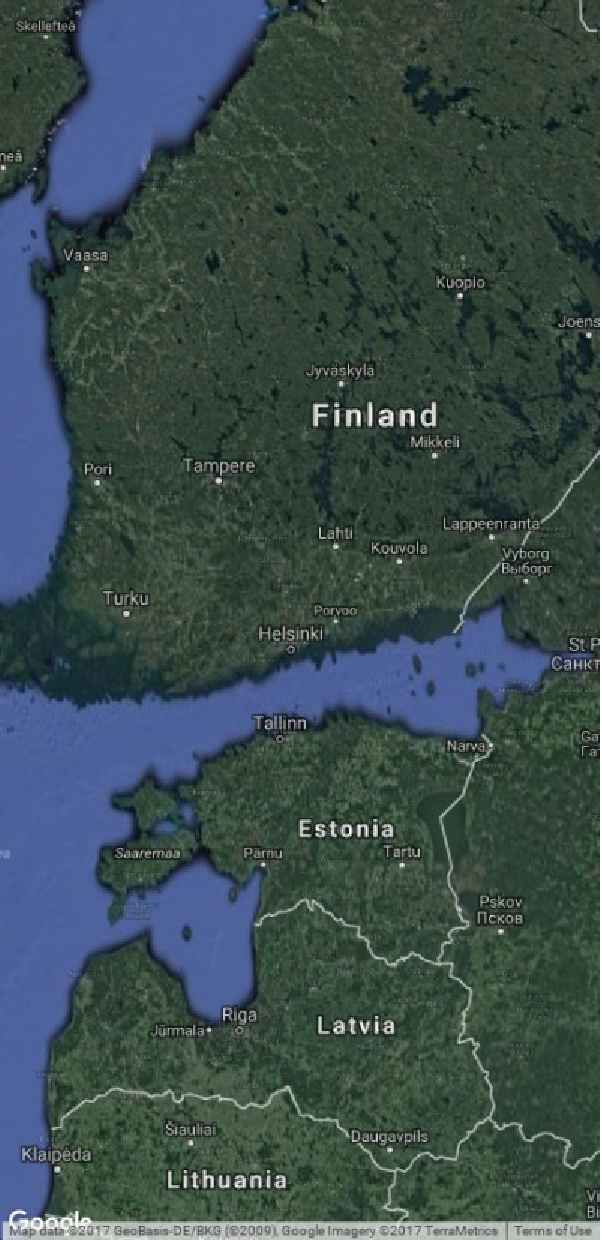
\includegraphics[width=\textwidth]{thesis-figures/figures-qgis/fulltile-google}
    \caption{Full tile, Google true colour}
  \end{subfigure} \hfill
  \begin{subfigure}[t]{.24\textwidth}
    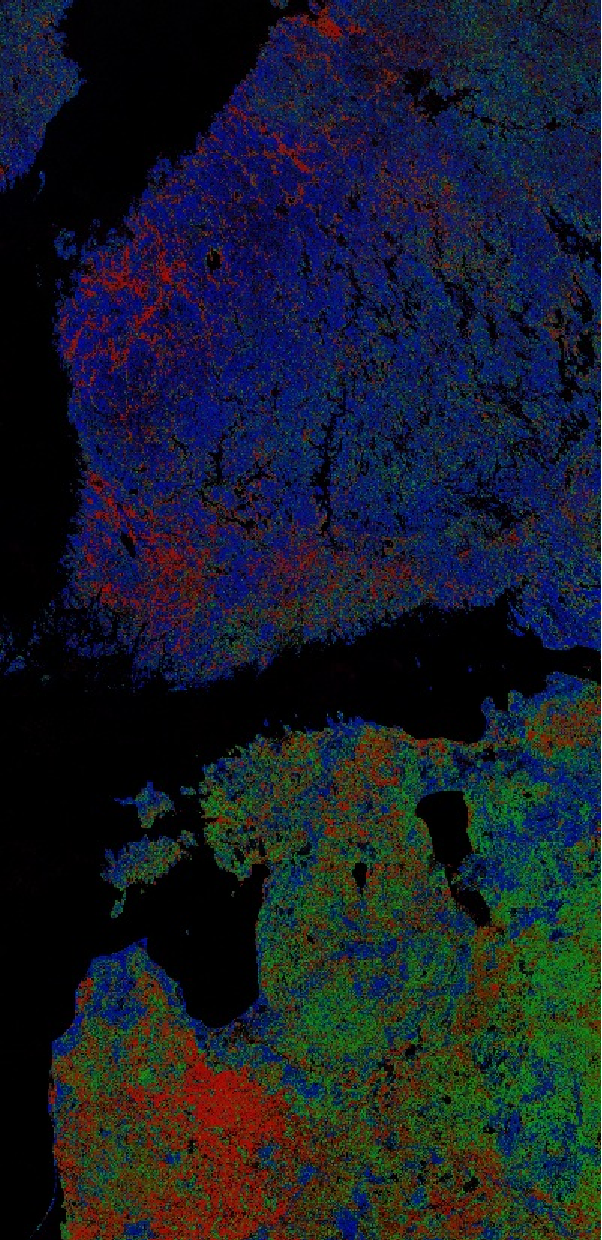
\includegraphics[width=\textwidth]{thesis-figures/figures-qgis/fulltile-rf}
    \caption{Full tile, random forest regression}
    \label{subfig-fulltile-rf}
  \end{subfigure} \hfill
  \begin{subfigure}[t]{.24\textwidth}
    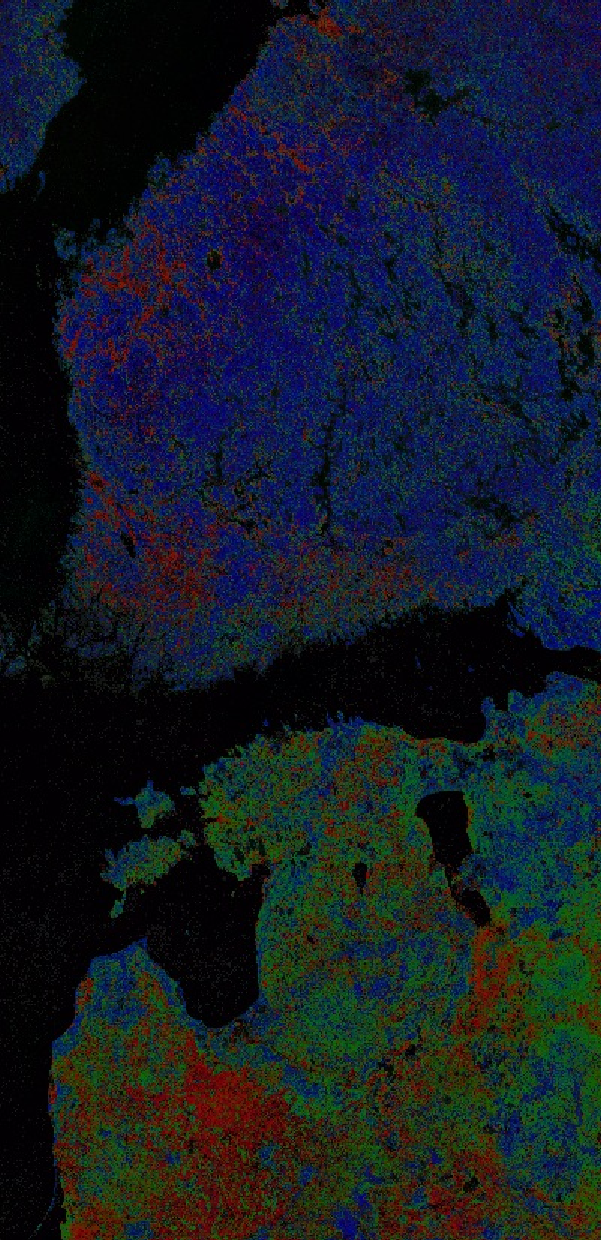
\includegraphics[width=\textwidth]{thesis-figures/figures-qgis/fulltile-nn}
    \caption{Full tile, neural networks}
  \end{subfigure} \hfill
  \begin{subfigure}[t]{.24\textwidth}
    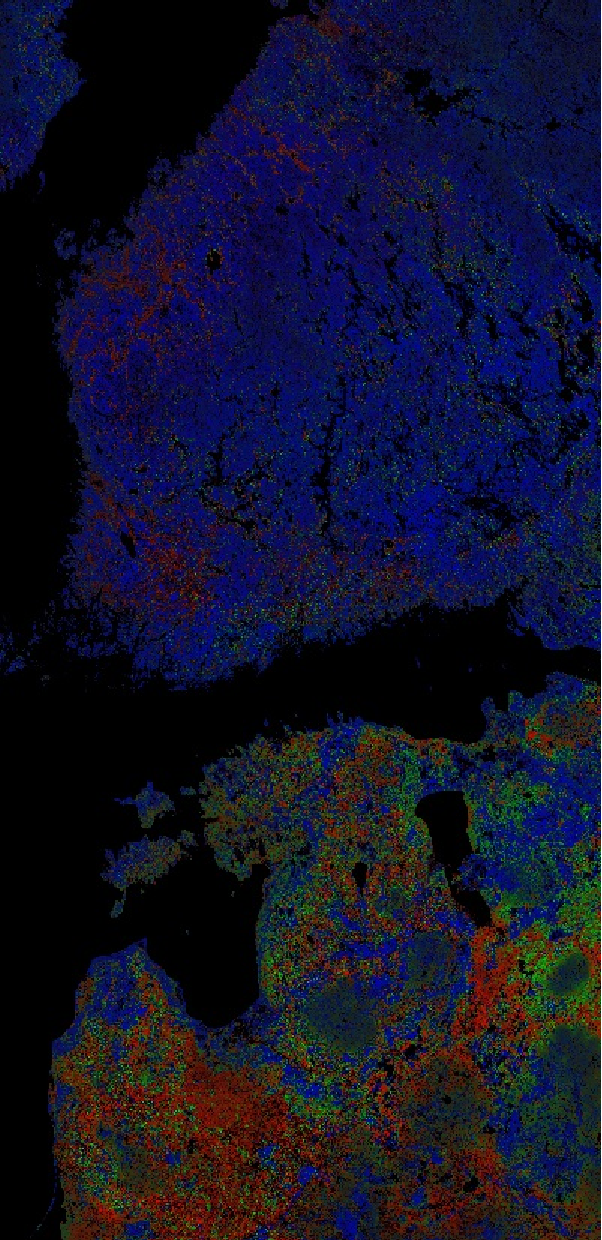
\includegraphics[width=\textwidth]{thesis-figures/figures-qgis/fulltile-cm}
    \caption{Full tile, fuzzy \textit{c}-means}
    \label{subfig-fulltile-cm}
  \end{subfigure} \
  \caption{Visual comparison of fuzzy classification prediction output. b-d red, green and blue colour channels represent cultivated, deciduous tree and evergreen tree class proportions, respectively.}
\end{sidewaysfigure}

\begin{sidewaysfigure}
  \ContinuedFloat
  \centering
  \begin{subfigure}[t]{.24\textwidth}
    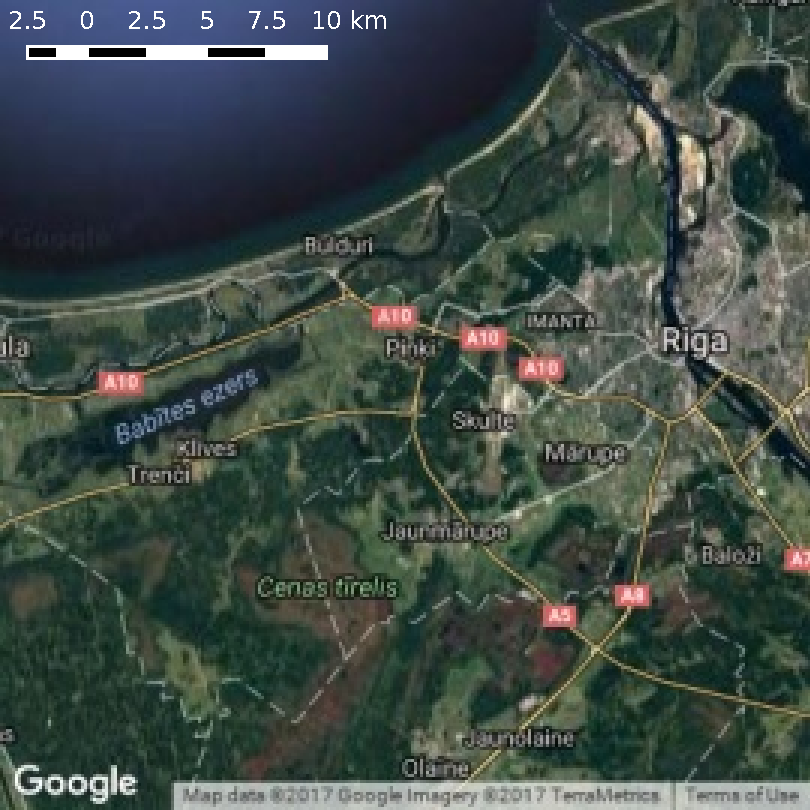
\includegraphics[width=\textwidth]{thesis-figures/figures-qgis/riga-google}
    \caption{R\={\i}ga, Google true colour}
  \end{subfigure} \hfill
  \begin{subfigure}[t]{.24\textwidth}
    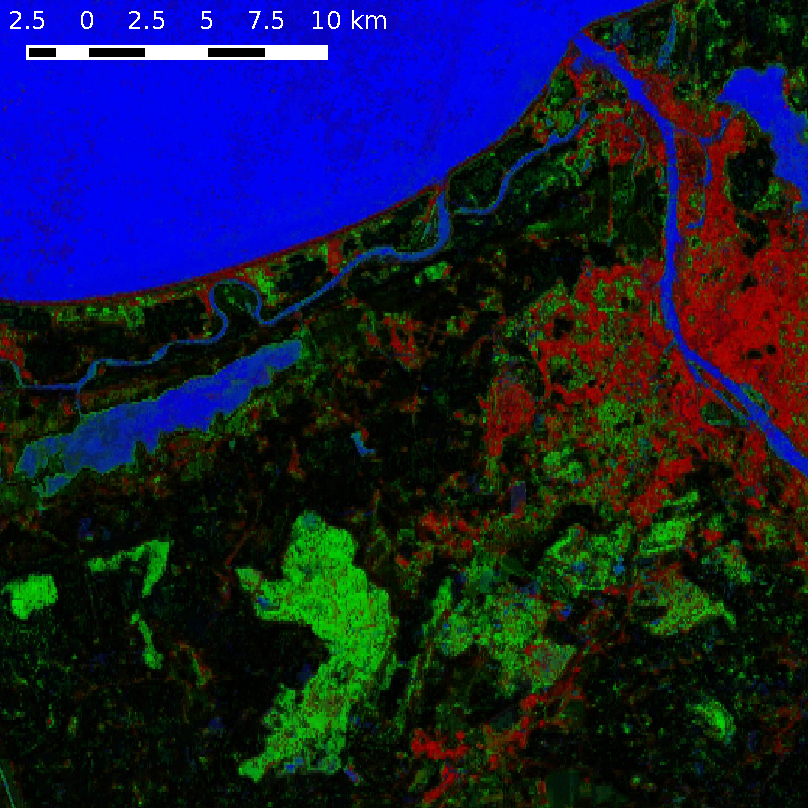
\includegraphics[width=\textwidth]{thesis-figures/figures-qgis/riga-rf}
    \caption{R\={\i}ga, random forest regression}
    \label{subfig-riga-rf}
  \end{subfigure} \hfill
  \begin{subfigure}[t]{.24\textwidth}
    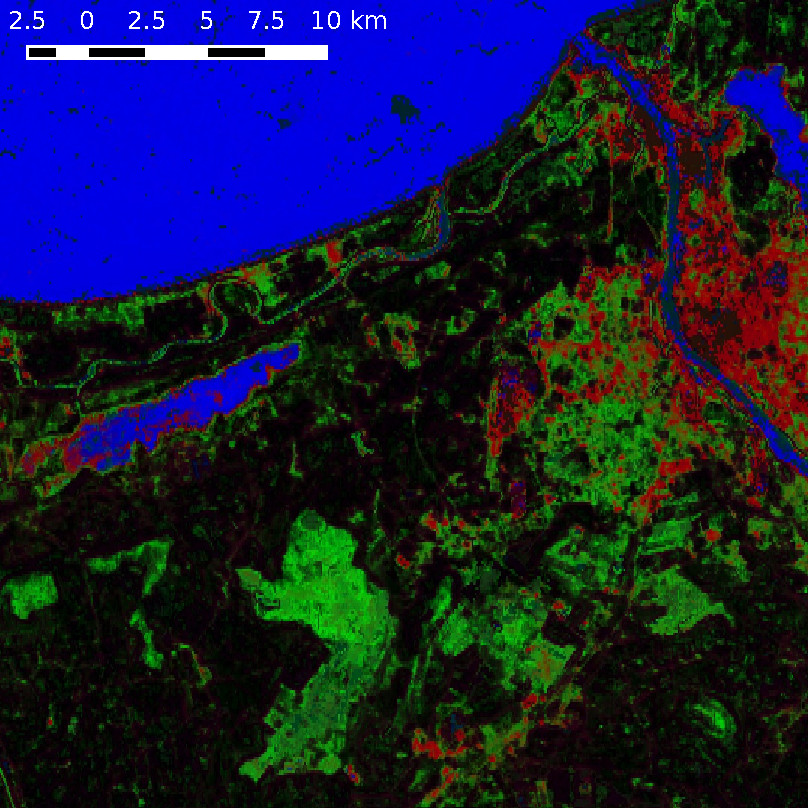
\includegraphics[width=\textwidth]{thesis-figures/figures-qgis/riga-nn}
    \caption{R\={\i}ga, neural networks}
    \label{subfig-riga-nn}
  \end{subfigure} \hfill
  \begin{subfigure}[t]{.24\textwidth}
    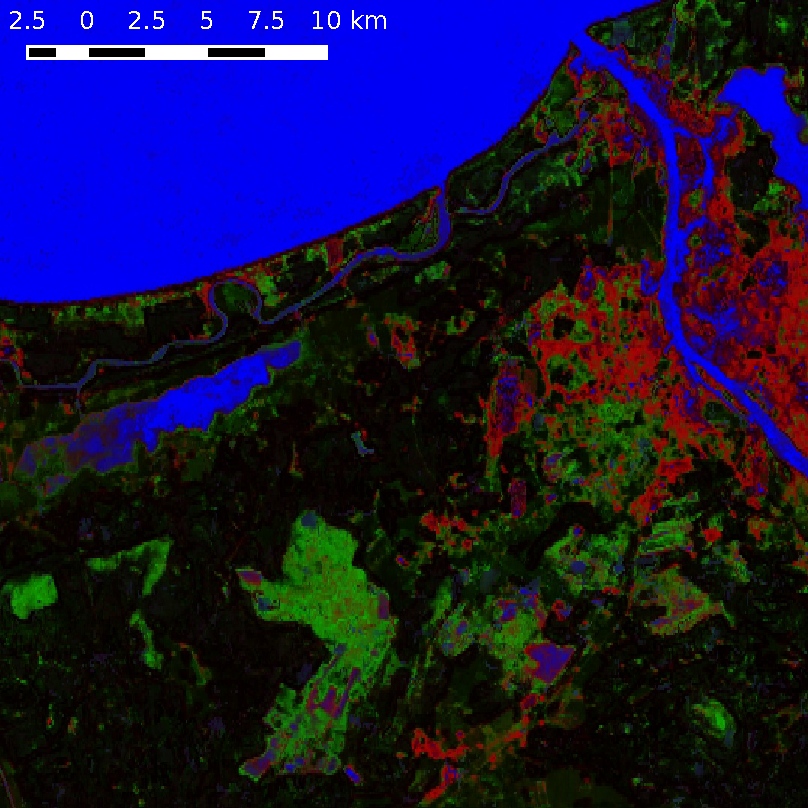
\includegraphics[width=\textwidth]{thesis-figures/figures-qgis/riga-cm}
    \caption{R\={\i}ga, fuzzy \textit{c}-means}
    \label{subfig-riga-cm}
  \end{subfigure} \
  \begin{subfigure}[t]{.24\textwidth}
    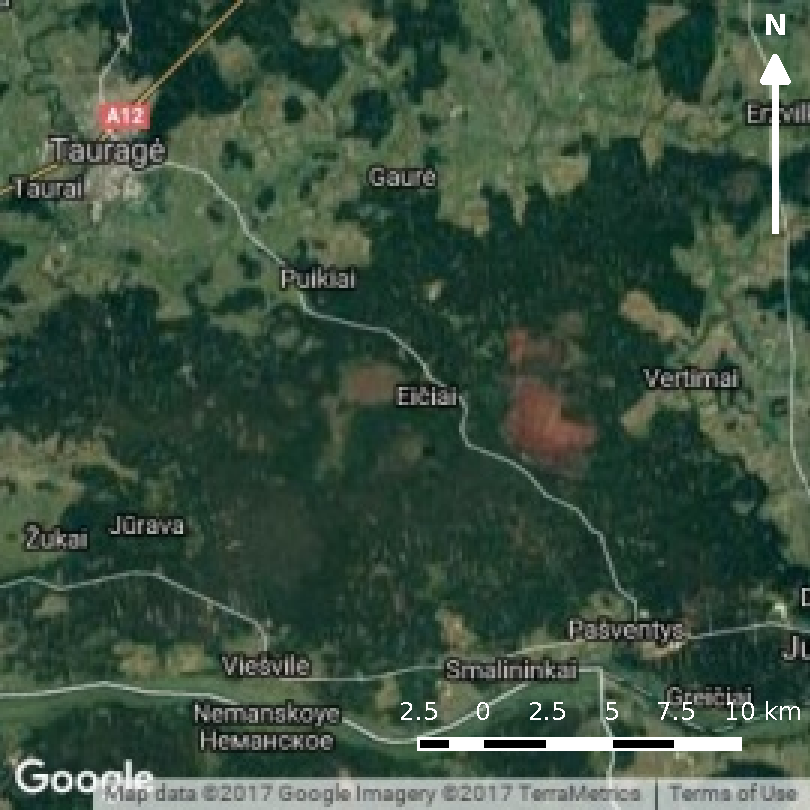
\includegraphics[width=\textwidth]{thesis-figures/figures-qgis/karsuva-google}
    \caption{Kar\v{s}uva, Google true colour}
  \end{subfigure} \hfill
  \begin{subfigure}[t]{.24\textwidth}
    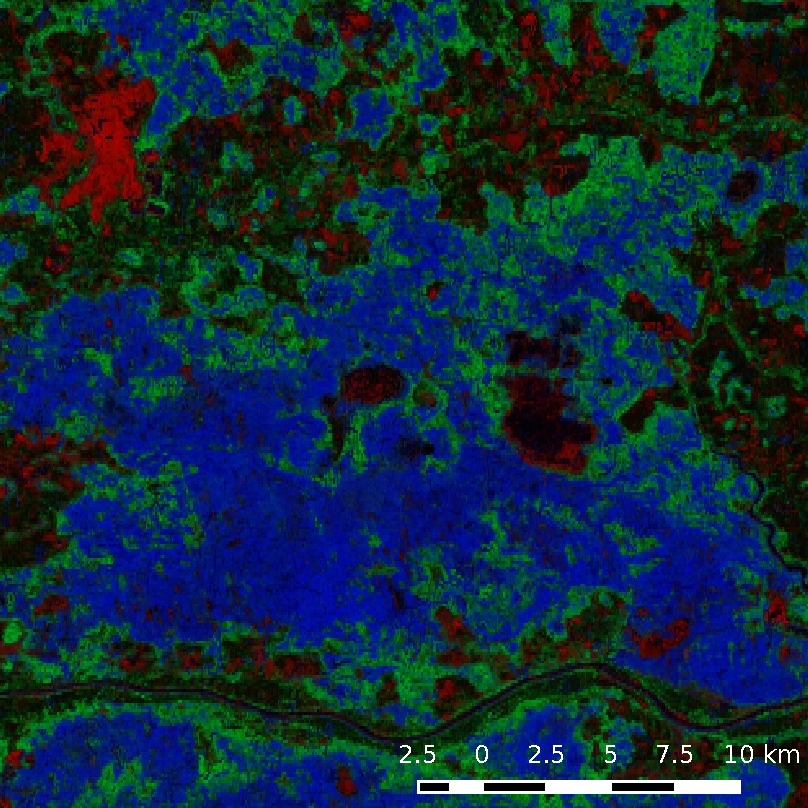
\includegraphics[width=\textwidth]{thesis-figures/figures-qgis/karsuva-rf}
    \caption{Kar\v{s}uva, random forest regression}
    \label{subfig-karsuva-rf}
  \end{subfigure} \hfill
  \begin{subfigure}[t]{.24\textwidth}
    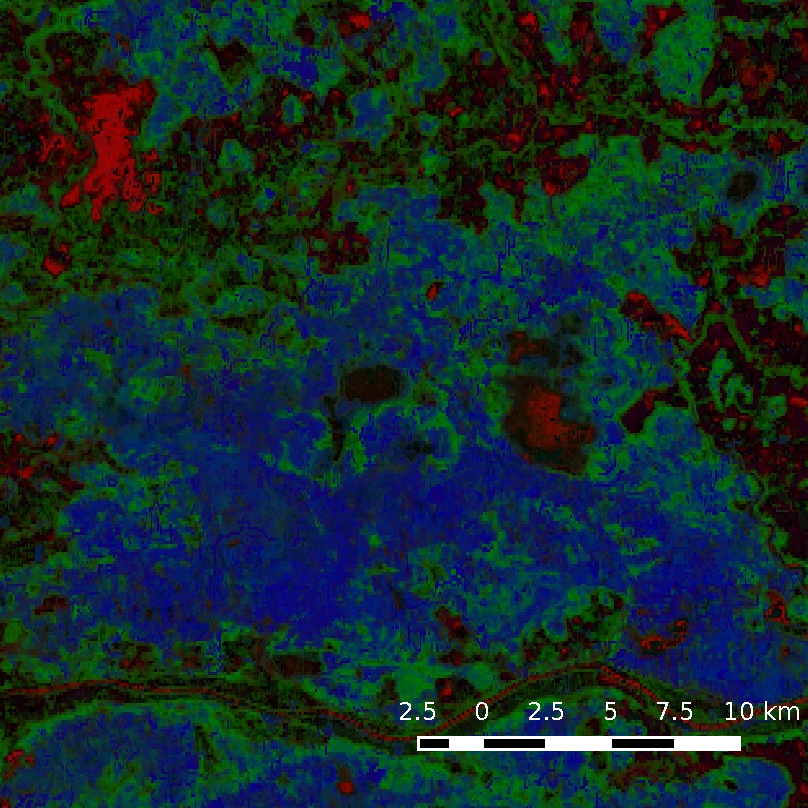
\includegraphics[width=\textwidth]{thesis-figures/figures-qgis/karsuva-nn}
    \caption{Kar\v{s}uva, neural networks}
  \end{subfigure} \hfill
  \begin{subfigure}[t]{.24\textwidth}
    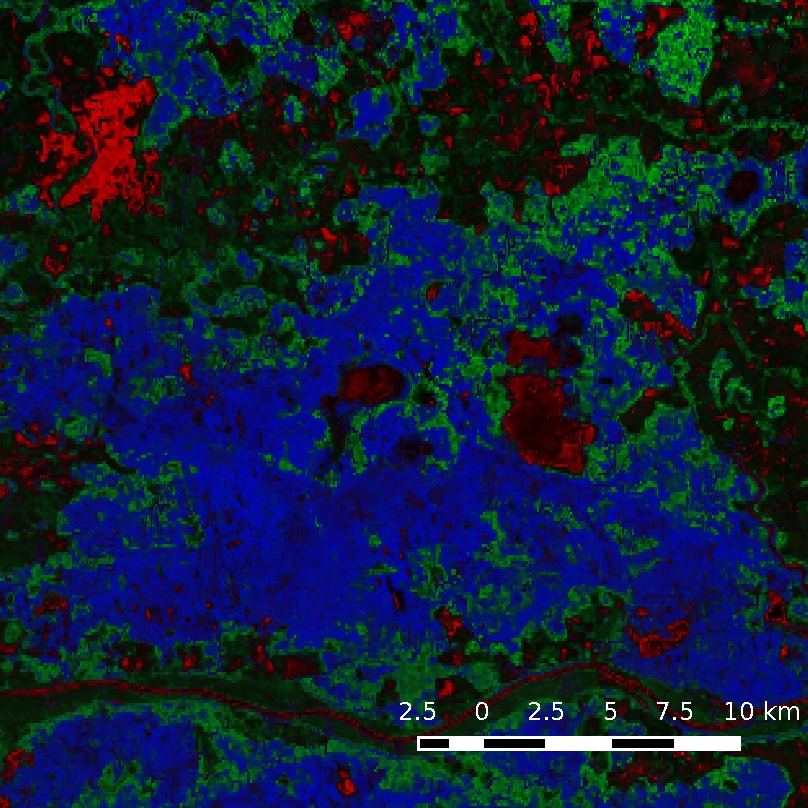
\includegraphics[width=\textwidth]{thesis-figures/figures-qgis/karsuva-cm}
    \caption{Kar\v{s}uva, fuzzy \textit{c}-means}
    \label{subfig-karsuva-cm}
  \end{subfigure} \
  \caption{Visual comparison of fuzzy classification prediction output. Red, green and blue colour channels represent: f-h: built-up, wetlands, water; j-l: built-up, deciduous trees, evergreen trees, respectively.}
\end{sidewaysfigure}

\begin{sidewaysfigure}
  \ContinuedFloat
  \centering
  \begin{subfigure}[t]{.24\textwidth}
    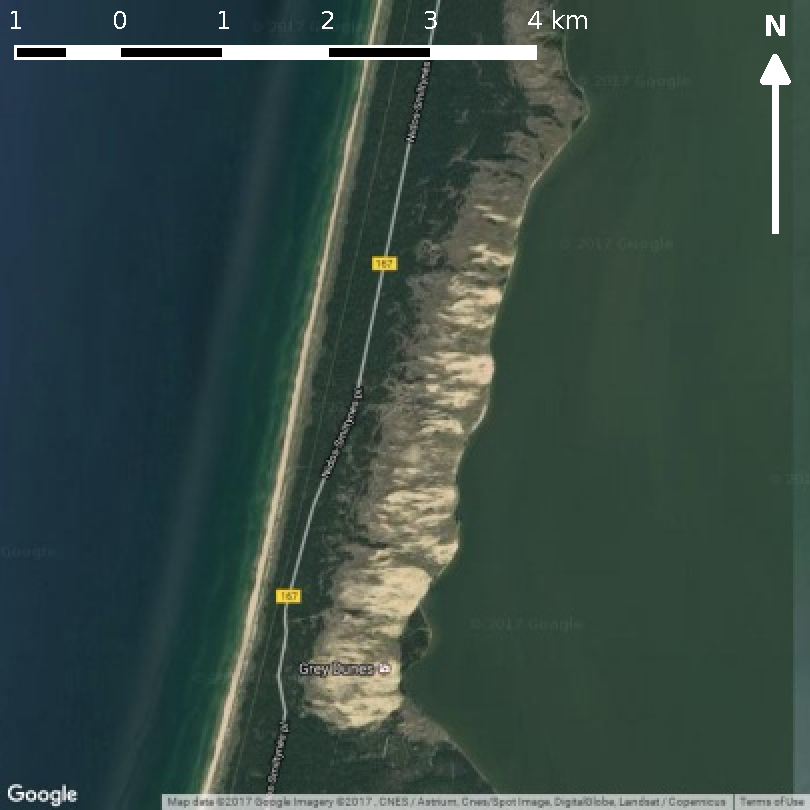
\includegraphics[width=\textwidth]{thesis-figures/figures-qgis/kursiunerija-google}
    \caption{Curonian spit, Google true colour}
  \end{subfigure} \hfill
  \begin{subfigure}[t]{.24\textwidth}
    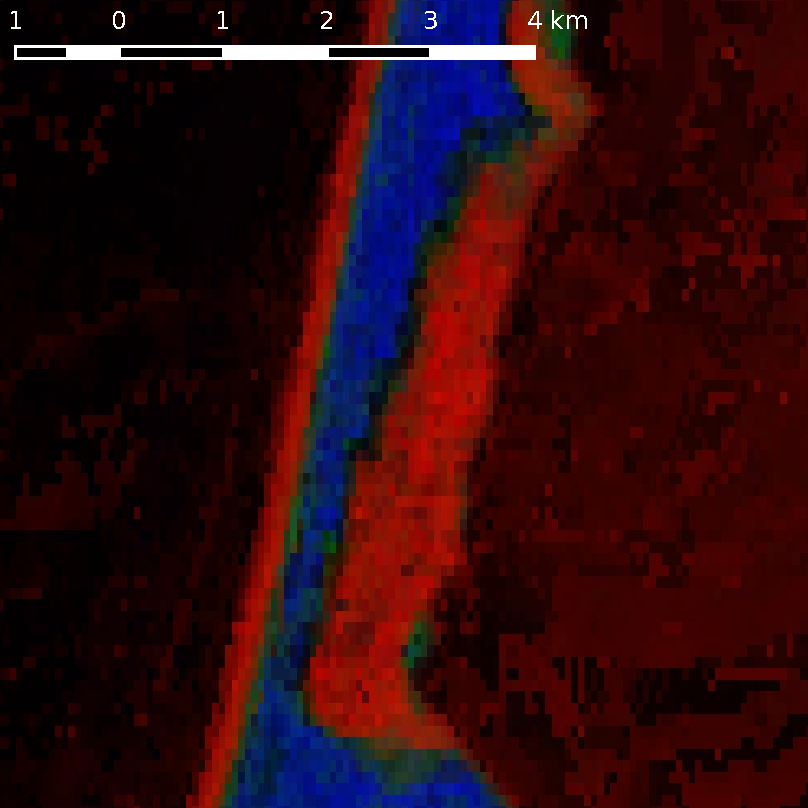
\includegraphics[width=\textwidth]{thesis-figures/figures-qgis/kursiunerija-rf}
    \caption{Curonian spit, random forest regression}
    \label{subfig-kursiunerija-rf}
  \end{subfigure} \hfill
  \begin{subfigure}[t]{.24\textwidth}
    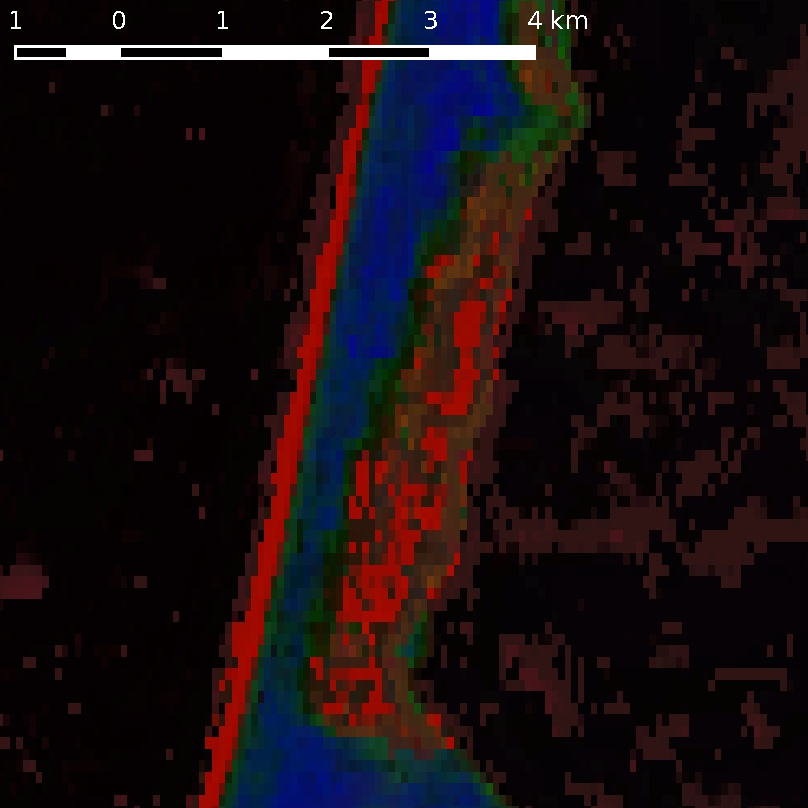
\includegraphics[width=\textwidth]{thesis-figures/figures-qgis/kursiunerija-nn}
    \caption{Curonian spit, neural networks}
    \label{subfig-kursiunerija-nn}
  \end{subfigure} \hfill
  \begin{subfigure}[t]{.24\textwidth}
    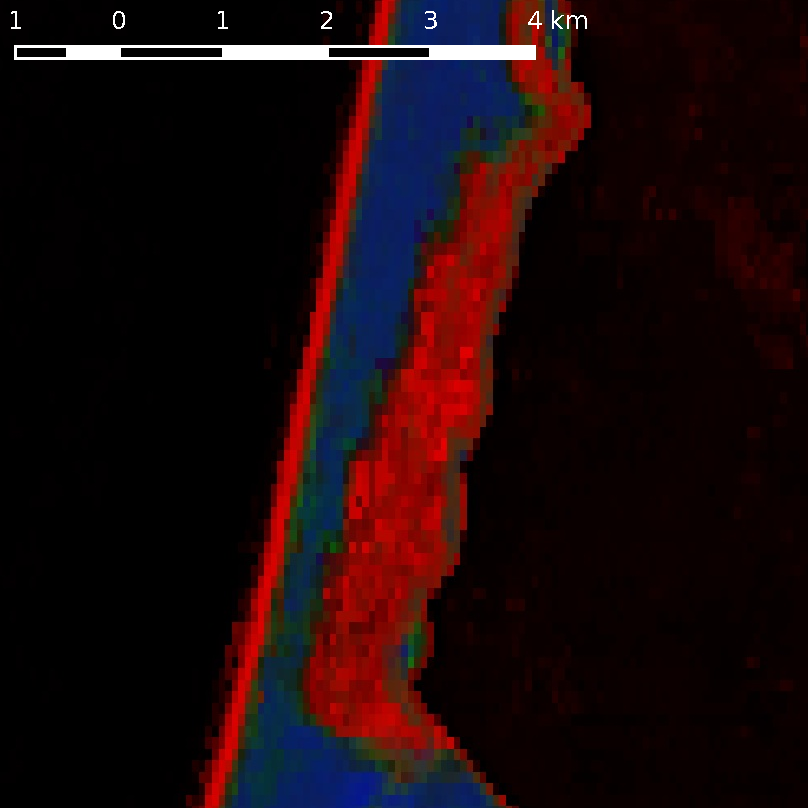
\includegraphics[width=\textwidth]{thesis-figures/figures-qgis/kursiunerija-cm}
    \caption{Curonian spit, fuzzy \textit{c}-means}
    \label{subfig-kursiunerija-cm}
  \end{subfigure} \
  \begin{subfigure}[t]{.24\textwidth}
    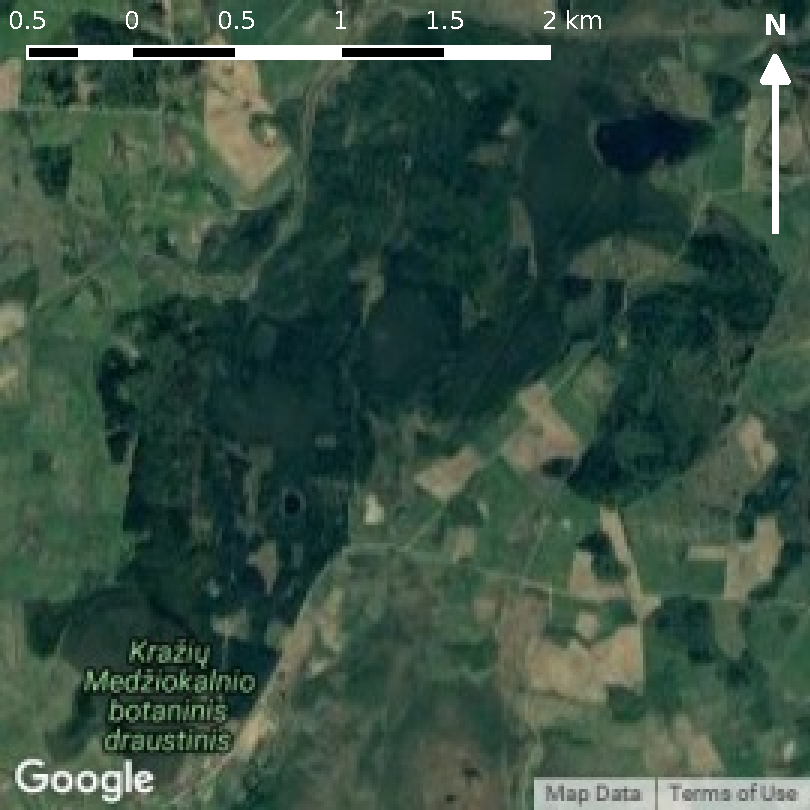
\includegraphics[width=\textwidth]{thesis-figures/figures-qgis/medziokalnis-google}
    \caption{Med\v{z}iokalnis, Google true colour}
  \end{subfigure} \hfill
  \begin{subfigure}[t]{.24\textwidth}
    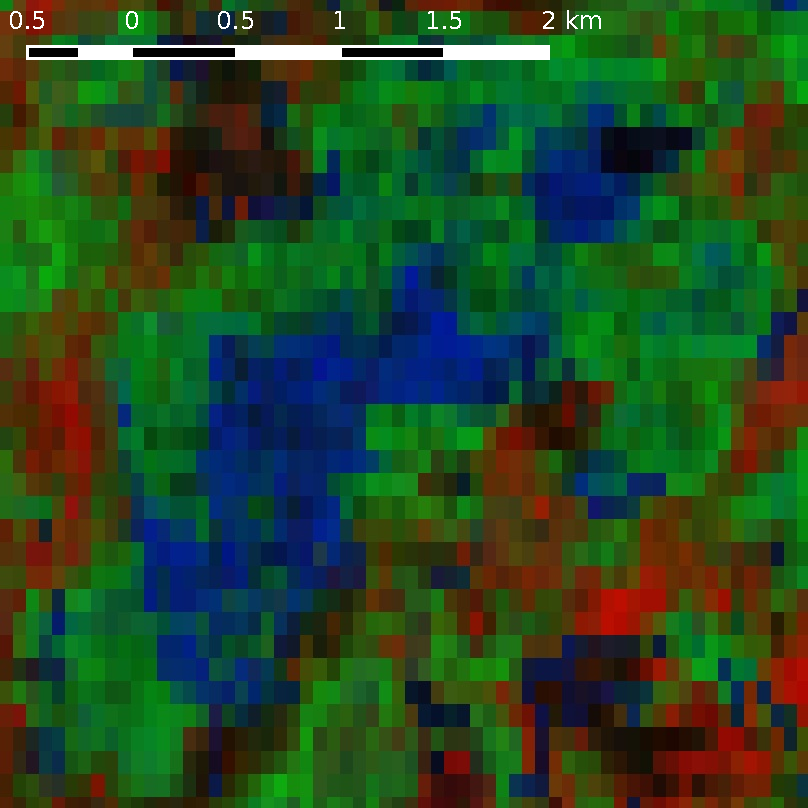
\includegraphics[width=\textwidth]{thesis-figures/figures-qgis/medziokalnis-rf}
    \caption{Med\v{z}iokalnis, random forest regression}
    \label{subfig-medziokalnis-rf}
  \end{subfigure} \hfill
  \begin{subfigure}[t]{.24\textwidth}
    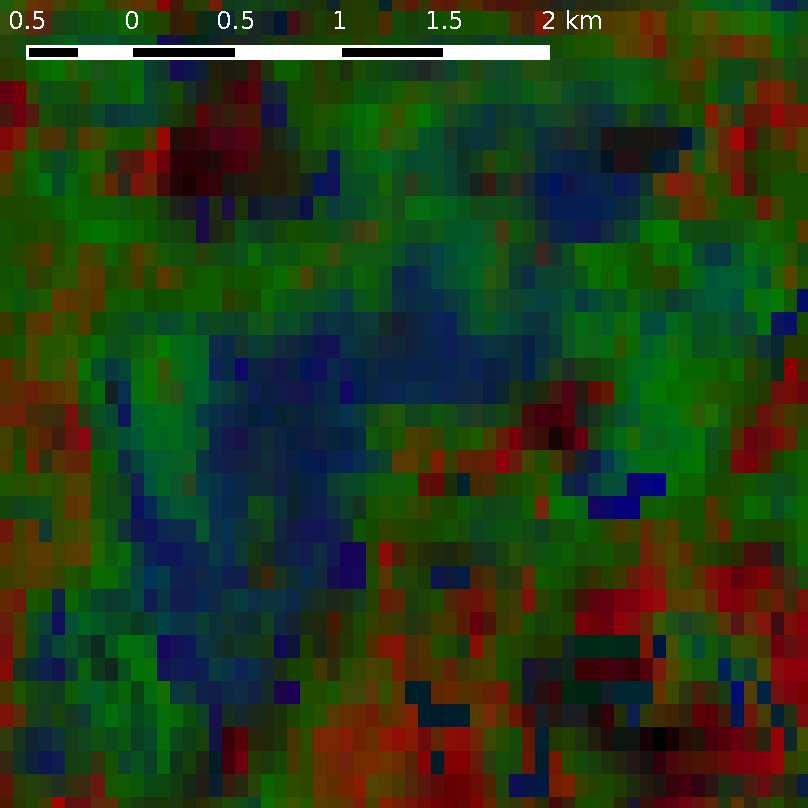
\includegraphics[width=\textwidth]{thesis-figures/figures-qgis/medziokalnis-nn}
    \caption{Med\v{z}iokalnis, neural networks}
  \end{subfigure} \hfill
  \begin{subfigure}[t]{.24\textwidth}
    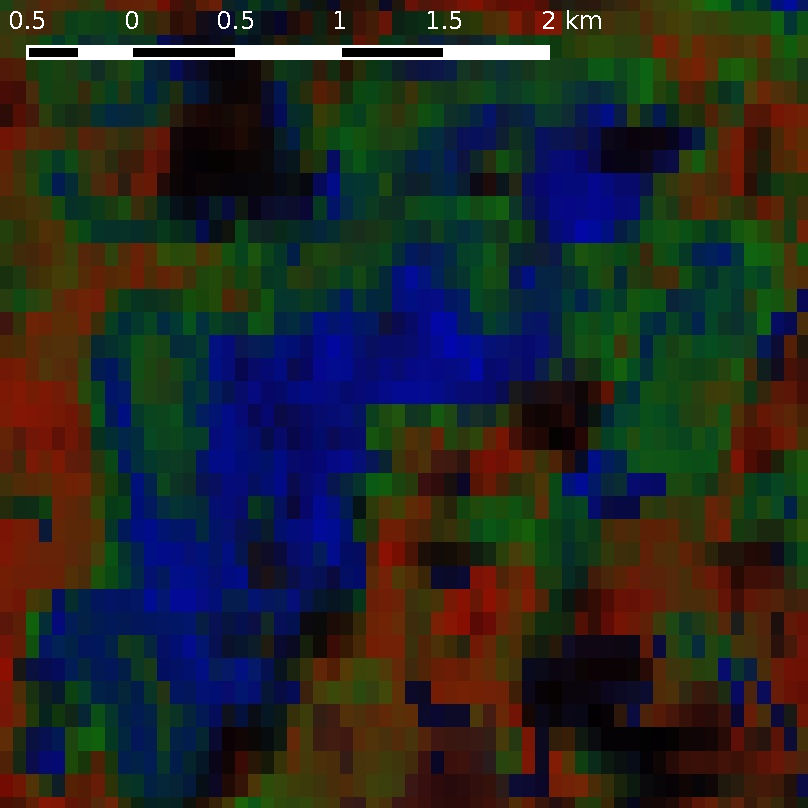
\includegraphics[width=\textwidth]{thesis-figures/figures-qgis/medziokalnis-cm}
    \caption{Med\v{z}iokalnis, fuzzy \textit{c}-means}
    \label{subfig-medziokalnis-cm}
  \end{subfigure} \
  \caption{Visual comparison of fuzzy classification prediction output. Red, green and blue colour channels represent: n-p: barren, grass, evergreen trees; r-t: cultivated, deciduous trees, evergreen trees, respectively.}
  \label{fig-visualcomparison}
\end{sidewaysfigure}

To better visualise the differences between the fuzzy classification methods, predictions were made using each method for the whole study area. See figure \ref{fig-visualcomparison} for some examples. Overall visual comparison confirms that the differences between the methods are minor. However, the differences are easier to spot with a side-by-side comparison.

As seen in figures \ref{subfig-fulltile-rf}-\ref{subfig-fulltile-cm}, all three fuzzy classification methods that could be trained on all pixels predicted a similar gradient for cultivated areas (red), which are more abundant in the south with large accumulation in more fertile areas in Latvia and Lithuania, and less abundant in the north, situated around rivers in Finland. However, fuzzy \textit{c}-means predicted fewer cultivated areas in Finland compared to the other two methods, and random forest regression tended to predict a larger proportion of cultivated area in a pixel compared to the other two methods. The distribution pattern of deciduous trees (green) was also similar, they were predicted to be more abundant in the south (Estonia, Latvia and Lithuania) and rare in the north (Finland). Fuzzy \textit{c}-means tended to predict fewer deciduous trees. Evergreen trees (blue) were predicted to follow the opposite pattern, as they are less common in the south and more abundant in the north. Note that latitude was not used as a covariate; such gradient patterns have emerged without it.

Figures \ref{subfig-riga-rf}-\ref{subfig-riga-cm} show the surroundings of the city of R\={\i}ga, Latvia. It includes lake Babites, a shallow lagoon-type lake whose edges are covered by reeds and bulrushes. It also shows a number of marshes, largest of which is Cenas tirelis, a protected \textit{Natura 2000} territory with peat extraction operations being performed in the southern part of the marsh. At this scale the differences between the fuzzy classification methods are also not large, but noticeable. Neural networks tend to predict fewer built-up areas (red) compared to the other two methods, and instead tends to predict too many wetlands (green), which is not as accurate. Neural networks also predict built-up areas on the edges of lake Babites, unlike the more appropriate classification as wetlands done by random forest regression. Fuzzy \textit{c}-means also predicts built-up areas there, but at a smaller proportion compared to neural networks. Fuzzy \textit{c}-means also tends to overestimate the proportion of built-up areas in peat extraction sites and water in built-up areas.

Figures \ref{subfig-karsuva-rf}-\ref{subfig-karsuva-cm} show Kar\v{s}uvos wood, fourth largest continuous forest in Lithuania, which consists of 60\% pine forest, 18\% spruce forest, 12\% birch forest and 9\% black alder (\textit{Alnus glutinosa} (L.) Gaertn.) forest \citep{lietuviuenciklopedija2006}. The fuzzy classification predictions show the expected pattern of the majority of the forest being classified as evergreen trees (blue), although fuzzy \textit{c}-means predicts more and neural networks predict less area covered by them. Likewise fuzzy \textit{c}-means predicts less and neural networks predict more deciduous tree (green) coverage. At the north-west corner of the figures all of the fuzzy classification methods correctly identify the town of Taurag\.{e} as a built-up area (red). However, all of the classification methods also show various amounts of built-up areas in the eastern part of the figures, which in reality is a peat extraction operation instead.

Figures \ref{subfig-kursiunerija-rf}-\ref{subfig-kursiunerija-cm} show grey dunes in the Curonian spit, Lithuania. This area is a sandy spit surrounded by water from both sides: the Curonian lagoon to the east and the Baltic sea to the west. It features a number of sand dunes that are not covered by vegetation, whereas the grey dunes are in the process of being covered by short herbaceous vegetation such as heath. The rest of the spit is covered largely by pine forests. The fuzzy classification methods mostly predict the grey dunes as the barren class (red), including parts that are now covered by grasses, with the exception of neural networks that tend to predict a mix of all classes in the parts covered by grass. The different methods all tend to correctly predict grass (green) around the edges of the dunes as well as the beach. Evergreen trees (blue) in pine forests are predicted by all classification methods correctly. A noticeable difference between the method results is the water, which appears as somewhat red in both the random forest regression and neural network case, especially the more shallow Curonian lagoon, indicating that those two methods predict a fraction of barren cover in the water. Fuzzy \textit{c}-means tends to do better in that regard overall, with fewer artefacts like that appearing in areas completely covered by water.

Figures \ref{subfig-medziokalnis-rf}-\ref{subfig-medziokalnis-cm} show the area of Med\v{z}iokalnis, a hill in western Lithuania covered by a mixed forest, parts of which are also a botanical reserve. The patterns on prediction by each of the fuzzy classification methods are very similar, with the main point of disagreement being the botanical reserve (south-west of the image) itself. Fuzzy \textit{c}-means predicts that the reserve consists mostly of evergreen trees (blue), whereas random forest regression predicts that it consists of deciduous trees (green). Just like in figure \ref{subfig-karsuva-cm}, fuzzy \textit{c}-means tends to predict more evergreen tree cover compared to the other methods. Neural networks predictions are more fuzzy than those of the other methods, with smoother transitions between pixels. Pixels being less saturated also shows that the percentage of the particular class predicted in the pixel is lower than in the other methods. Another place of disagreement is a large agriculture field at the north-west, which is not at all classified as cultivated area (red) by fuzzy \textit{c}-means, but classified (partly) as such by neural networks.

\begin{figure}
  \centering
  \begin{subfigure}[t]{0.49\textwidth}
    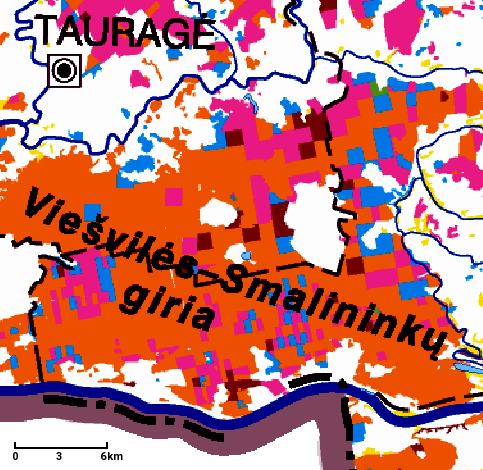
\includegraphics[width=\textwidth]{thesis-figures/karsuva-atlas}
    \caption{Wood of Kar\v{s}uva, also known as Vie\v{s}vil\.{e}s-Smalinink\k{u} wood}
  \end{subfigure} \hfill
  \begin{subfigure}[t]{0.45\textwidth}
    
\includegraphics[width=\textwidth]{thesis-figures/medziokalnis-atlas}
    \caption{Med\v{z}iokalnis forest}
  \end{subfigure}
  \caption{Forest dominant species distribution as per the National Atlas of Lithuania \citep{treeatlas2011}. Pink: Norway spruce, orange: scots pine, light blue: birch, yellow: grey alder \textit{Alnus incana} (L.) Moench, brown: black alder, green: ash \textit{Fraxinus excelsior} L., dark blue: river (including labels, such as \textit{Kra\v{z}ant\.{e}}), cyan: lake.}
  \label{fig-atlas-forest}
\end{figure}

Tree type prediction accuracy can be validated with national atlas data (see figure \ref{fig-atlas-forest}). In the case of both forests, fuzzy \textit{c}-means prediction appears to be the most accurate, since it does not overestimate the proportion of deciduous trees. However, in the case of Med\v{z}iokalnis forest, random forest regression is the most accurate in predicting deciduous trees in the south-west part (botanical reserve). Note that the atlas data is from 2011, whereas this study was performed on 2014-2016 data, so the patterns should not be expected to match perfectly.

\begin{figure}
  \centering
  \begin{subfigure}[b]{0.48\textwidth}
    \centering
    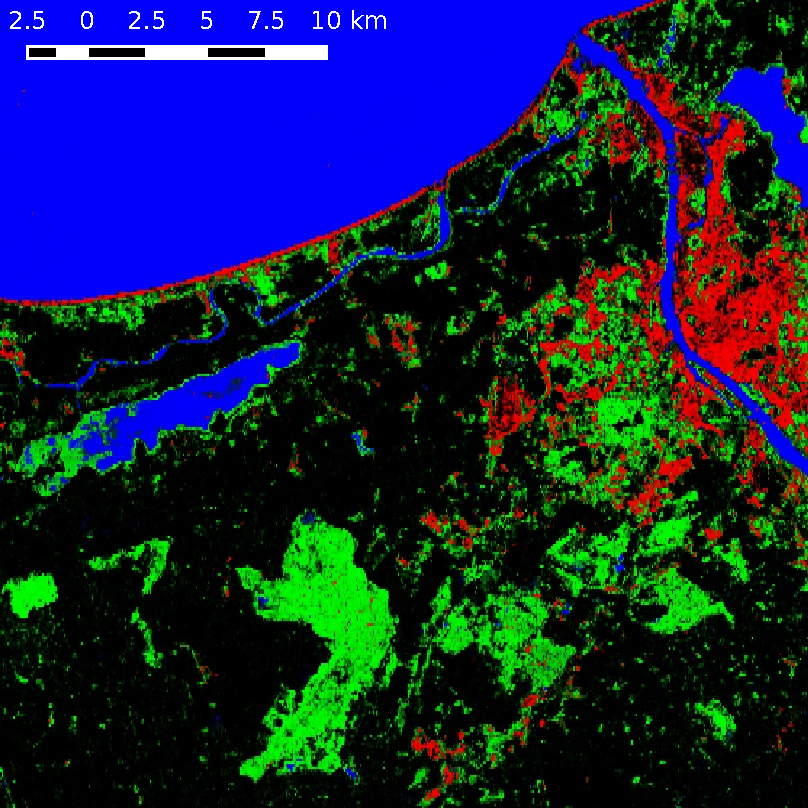
\includegraphics[width=0.8\textwidth]{thesis-figures/figures-qgis/riga-gbu}
    \caption{R\={\i}ga, unoptimised multiclass gradient boosting}
  \end{subfigure} \hfill
  \begin{subfigure}[b]{0.48\textwidth}
    \centering
    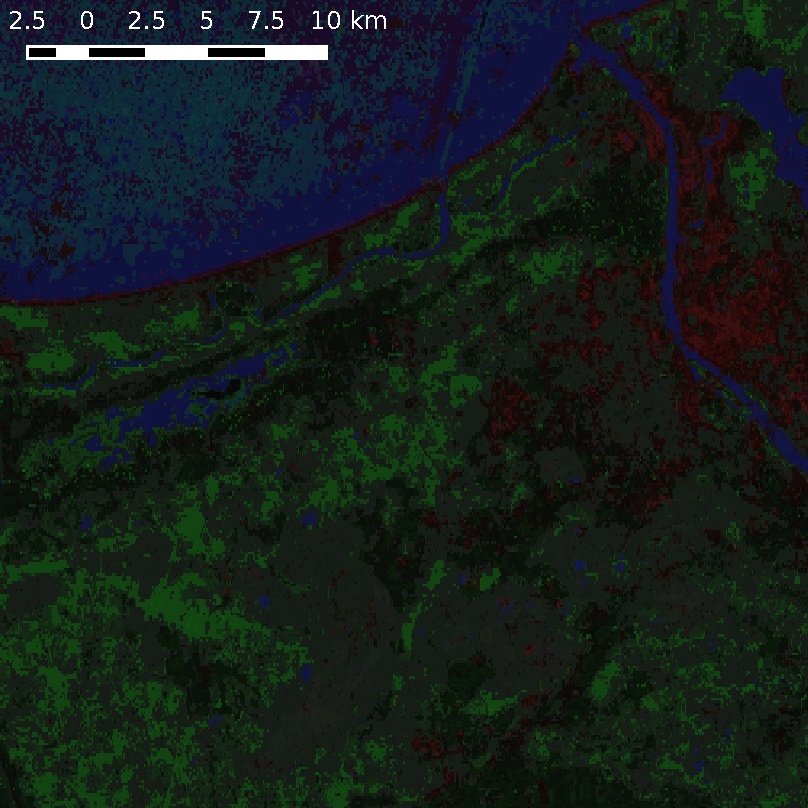
\includegraphics[width=0.8\textwidth]{thesis-figures/figures-qgis/riga-gbo}
    \caption{R\={\i}ga, optimised multiclass gradient boosting}
  \end{subfigure}
  \begin{subfigure}[b]{0.48\textwidth}
    \centering
    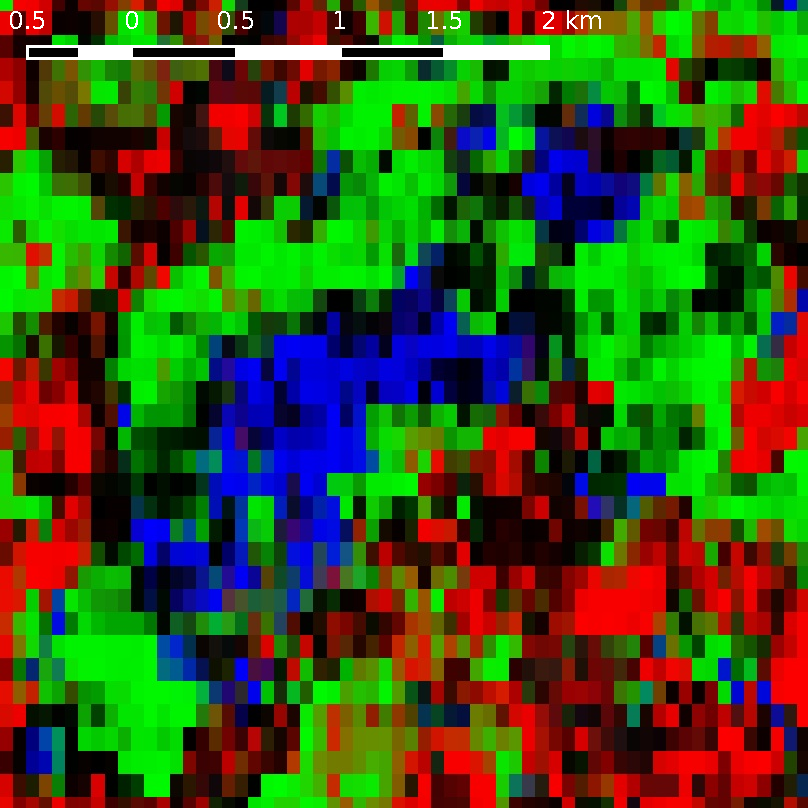
\includegraphics[width=0.8\textwidth]{thesis-figures/figures-qgis/medziokalnis-gbu}
    \caption{Med\v{z}iokalnis, unoptimised multiclass gradient boosting}
  \end{subfigure} \hfill
  \begin{subfigure}[b]{0.48\textwidth}
    \centering
    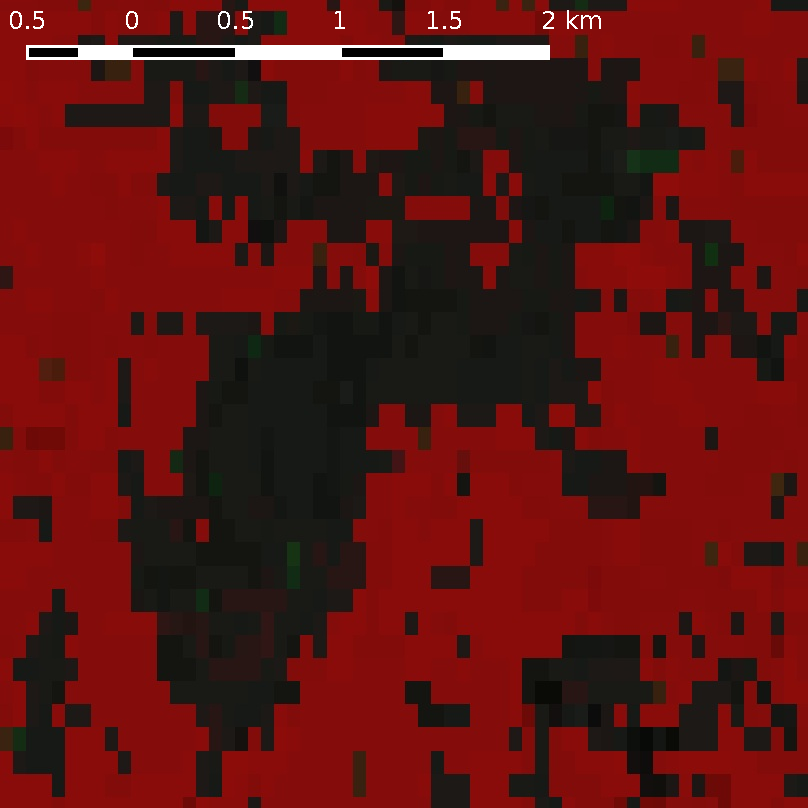
\includegraphics[width=0.8\textwidth]{thesis-figures/figures-qgis/medziokalnis-gbo}
    \caption{Med\v{z}iokalnis, optimised multiclass gradient boosting}
  \end{subfigure}
  \caption{Visual comparison of optimised and unoptimised multiclass gradient boosting prediction. Red, green and blue colour channels represent: a and b: built-up, wetlands, water; c and d: cultivated, deciduous tree and evergreen tree cover proportion, respectively.}
  \label{fig-gradientboost-comparison}
\end{figure}

In the case of multiclass gradient boosting, its prediction is not directly comparable to the ones of other fuzzy classification methods due to different training sets. However, an interesting observation can be made about the differences between optimised and unoptimised multiclass gradient boosting prediction results (see figure \ref{fig-gradientboost-comparison}). Since the optimal model was taken as the one with the lowest RMSE, and the unoptimised model is 7\% worse than the control (completely fuzzy set), optimisation strongly favoured increasing the fuzziness of the result. Thus in reality, the unoptimised model performs better than the optimised one, due to the latter being too fuzzy compared to the reality. However, the unoptimised model is also visibly too crisp.

\section{Covariate importance}
%TODO: Do I add x over y plots?

Covariates that were important for classification varied depending on the class (see figure \ref{fig-variable-importance}). The covariate that had the most importance for all classes was mean NDVI, and both the red band and near infrared bands were important for predicting most classes. The water mask, aspect and \nth{1} order phase were the least important. Some of the covariates had high importance for just one class, such as \nth{2} order amplitude for cultivated areas, \nth{2} order phase for wetlands, terrain position index for shrubs. Three covariates were confounding for some classes: \nth{2} order amplitude hindered shrub prediction, aspect hindered evergreen tree prediction and the water mask hindered wetland prediction.

\begin{figure}
  \centering
  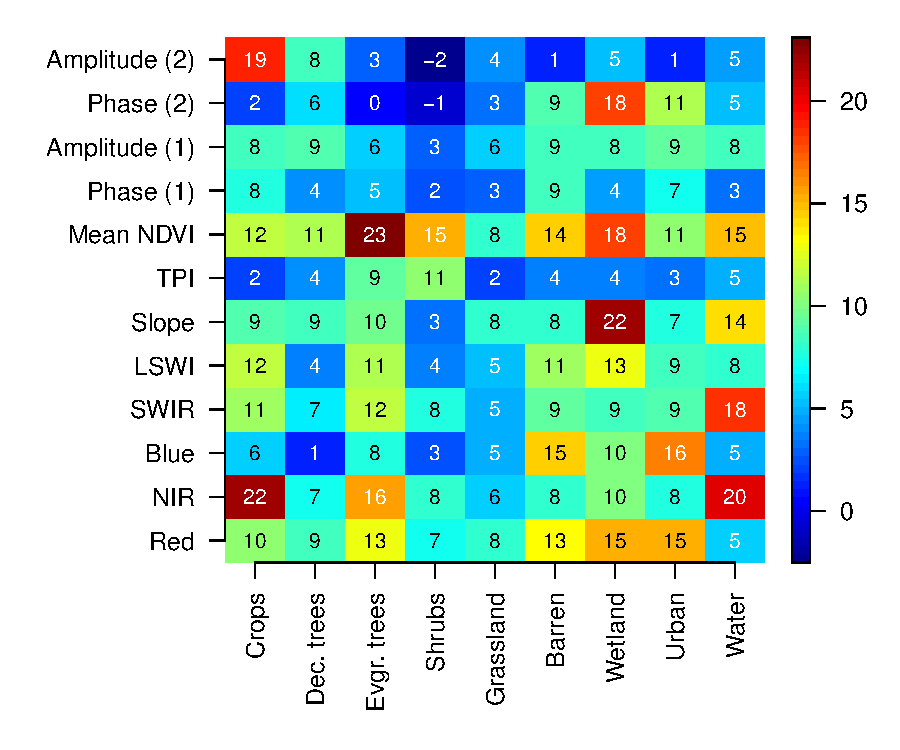
\includegraphics[width=0.72\textwidth]{thesis-figures/variable-importance}
  \caption{Covariate permutation importance for holdout random forest regression. Values indicate the increase in prediction RMSE when a given covariate is shuffled, thus higher values mean higher importance of the covariate.}
  \label{fig-variable-importance}
\end{figure}

The model optimisation step for each method involved dropping terms one by one until the overall RMSE no longer decreased. The terms dropped for each method are shown in table \ref{tbl-covariate-drop}. Aspect and the water mask hindered prediction accuracy for all methods; OSAVI hindered three, whereas TPI, elevation and amplitude of both orders hindered two of the four methods.

\begin{table}
  \centering
  \resizebox{\textwidth}{!}{
  \begin{tabular}{ll}
    Method & Covariates dropped\\ \hline
    Random forest regression & OSAVI, elevation, aspect, water mask\\
    Neural networks & Blue, OSAVI, aspect, TPI, amplitude of both orders, water mask\\
    Fuzzy \textit{c}-means & Red, blue, SWIR, LSWI, aspect, TPI, amplitude of both orders, water mask\\
    Multiclass gradient boosting & SWIR, OSAVI, LSWI, elevation, aspect, water mask\\
  \end{tabular}
  }
  \caption{Covariates dropped in the model optimisation step for each method.}
  \label{tbl-covariate-drop}
\end{table}


\section{Training and prediction time}

\subsection{Training time}

The four algorithms tested, in terms of time required for model training, are quite different due to their unique approach. The easiest algorithm to train was fuzzy \textit{c}-means, since training for it comes down to calculating a weighted mean of all training samples in order to get the class centroids, as well as the standard deviation of them. This takes only 0.03 seconds on the VITO virtual machine.

The second easiest to train is random forest regression. The training time for it is dependent on the number of decision trees the model needs to generate, with the default being 500. For training on all 480 samples, this takes 0.25 seconds on average.

Both gradient boosting and neural networks do not have a predetermined training stop point, and can potentially train the model forever. The \texttt{neuralnet} function requires specifying both the maximum number of iterations for training as well as the error threshold at which to stop training the model. If the error threshold is not reached within the maximum number of iterations, model training is aborted. In addition, several repetitions of training are needed, since the initial neural network node weights are random and can effect whether the optimisation gets stuck in a local minimum or not. It takes some trial and error to determine a reasonable number of iterations and a threshold, depending on how long one is willing to wait for training. In this study, neural network training was run for around 20 seconds per repetition, for 10 repetitions, although depending on the random starting weights one repetition could reach the threshold in as short as 17 seconds or as long as 33 seconds.

For gradient boosting, the \texttt{xgboost} package employs a method where a model can be trained iteratively: after an initial run, the model parameters are saved on disk, so that a second run with identical parameters skips the initial training part and continues where it left off. However, in the case of this study, multiclass gradient boosting was only able to make use of endmember pixels, so it was very prone to overtraining. Increasing the amount of training iterations even past 5 would increase the RMSE of the resulting model. A lower number of steps results in a more fuzzy result (fewer extreme predictions of 100\% and 0\%), which is favourable for RMSE that penalises large errors. Training of multiclass gradient boosting for 5 iterations for the first time (before the model caching mechanism is activated) takes 149 seconds (user time), but since it employs multithreading for training, the wall clock time on the 32-thread virtual machine for this task is 7 seconds.

\subsection{Prediction time}

\begin{figure}
  \centering
  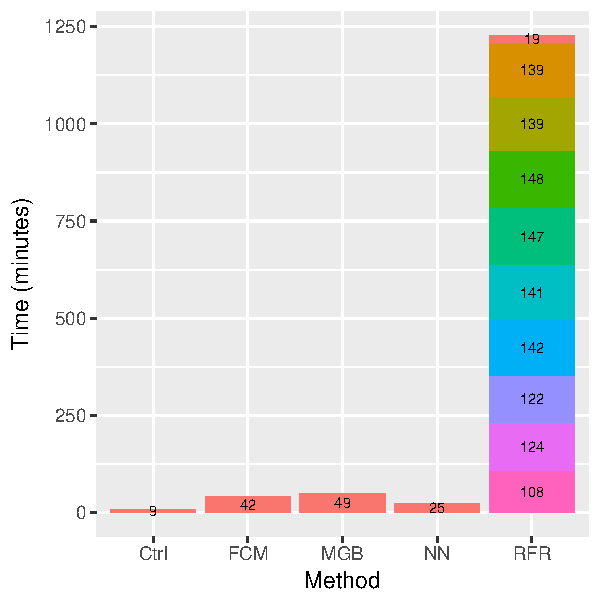
\includegraphics[width=0.6\textwidth]{thesis-figures/timing}
  \caption{Prediction user time for the different classification methods (Ctrl: control prediction of a fully fuzzy set 100\%/9; RFR: random forest regression; MGB: multiclass gradient boosting; FCM: fuzzy \textit{c}-means; NN: neural networks), using unoptimised variants (predictions done using all covariates). The different colours in random forest regression case show time needed to process each separate class layer, whereas all other methods process all layers at once.}
  \label{fig-timing}
\end{figure}

In order to compare the prediction time between classification methods, user time for the prediction step (using the \texttt{raster::predict} function) was measured, not counting the extra time needed for preprocessing of some data for the prediction. A control was also run, where the prediction function would always return \texttt{100/9}, in order to measure the overhead of the \texttt{raster::predict} function itself (see figure \ref{fig-timing}).

Most of the classification methods took 25-49 minutes to predict all 9 classes for each pixel of an entire PROBA-V tile (101,606,400 pixels), of which 9 minutes are attributable to the overhead of the \texttt{raster::predict} function itself. The random forest regression method, however, took much longer: even 20.5 hours. It needed 1.8-2.5 hours to predict the proportion of each individual class, and 19 more minutes to postprocess the values so each pixel sums up to 100\%. The \texttt{raster::predict} overhead for an individual layer was 5 minutes.

Note that these results are in user time, which is the total time that a process takes to run on a single thread, not counting time spent by the kernel, such as file input/output. This is different from wall clock time, which is the actual time a task takes to complete; in multithreaded cases, wall clock time is shorter than user time. User time was used so as to be able to compare the methods no matter whether their respective packages implement multithreading or not. For instance, while random forest regression takes 25-50 times more user time compared to the other methods, it is multithreaded by default. The wall clock time of random forest regression was only 1 hour, showing a 20-times reduction in processing time needed on the PROBA-V MEP server (using 32 threads). However, current fuzzy \textit{c}-means and neural network implementations do not make use of multithreading yet.

In addition, the extra preprocessing steps needed before the prediction are not reflected in figure \ref{fig-timing}. These steps varied per classification method. For fuzzy \textit{c}-means, it involved separating the covariate rasters into 25 chunks and converting them into a \texttt{SpatialPixelsDataFrame}. For neural networks, it involved scaling all covariate rasters to the 0-1 range. For random forest regression, extra processing time was needed to store the individual layers on disk and then compress them all to one file. Nothing extra was required for multiclass gradient boosting.

\chapter{Discussion}

\section{Classification method accuracy comparison}

The differences between the four tested classification methods in terms of prediction accuracy were small, once the models were optimised, as evident from both from the error statistics (figure \ref{fig-total-errors}) and the visual comparison of a full-tile prediction (figure \ref{fig-visualcomparison}). This indicates that the method itself is not so much important as the data that the models can train on, which is in line with the conclusions of \citet{yu2014metadiscoveries}. However, this is true only after performing the optimisation step, which included adjusting the fuzziness of the result and dropping least important covariates, to get the most out of each method. This optimisation step helped improve prediction accuracy, but at a varying degree: 13\% for fuzzy \textit{c}-means, but only 1\% for random forest regression.

Even though the differences between the methods were small, overall random forest regression gave the best results, both in terms of error statistics and visual comparison. The binary relevance method used for random forest was expected to hinder the prediction accuracy, as the algorithm cannot use the information about the proportions of other land cover classes than the one being modelled. However, the results indicate that this issue is not a concern after all. In addition, since the binary relevance method requires separate models per class, this brings the opportunity to further optimise these models for their respective classes, for instance by performing per-class term selection. Moreover, the per-class mean errors (bias) of random forest regression were very low compared to other classification methods, indicating that it did not tend to overestimate or underestimate any particular classes. Lastly, model optimisation resulted in only 1\% decrease in prediction RMSE, which indicates that random forest is capable of dealing with poorly predictive covariates. This may make the optimisation step unnecessary, which would in turn speed up the training process, as term selection and parameter tuning may be skipped for little loss in prediction accuracy. This confirms the findings of \citet{Pelletier2016hardrf} and \citet{breiman2001random} that random forest is particularly insensitive to parametrisation and covariates of little importance, rather than the findings of \citet{walton2008subpixelrf} who concludes that it is just as sensitive to covariates as other classification methods.

Neural networks were expected to have the best prediction accuracy, since they are capable of handling multiple input and multiple output data and is thus a fully fuzzy classification approach \citep{zhang2001fullyfuzzy}. However, its predictions turned out to be less accurate than expected. In particular, visual comparison of the prediction results shows that neural networks tend to overestimate the proportion of wetlands and tend to confuse water with built-up areas (figure \ref{subfig-riga-nn}). The predictions of neural networks were also the least smooth, with obvious artefacts in some cases (figure \ref{subfig-kursiunerija-nn}). This is possibly due to how difficult it is to train neural networks. All input data needs to be rescaled to the 0-1 range and covariates with little explanatory value have to be dropped for it to perform well, but this preprocessing by itself has the downside of making the algorithm easily affected by outliers in the data and not making use of all available data. Neural networks also have a large number of parameters, so extensive sensitivity analysis would be necessary to investigate the potential of neural networks in depth. Overall neural network predictions were less accurate, but not significantly, than fuzzy \textit{c}-means and random forest regression.

Fuzzy \textit{c}-means, which is also a fully fuzzy classification method \citep{zhang2001fullyfuzzy}, achieved a prediction accuracy almost on par with random forest regression, and slightly better than neural networks, although the differences were insignificant in both cases. This matches the findings of \citet{zhang2001fullyfuzzy}, who also found that fuzzy \textit{c}-means overall classification accuracy is insignificantly better than that of neural networks. Visual inspection shows that the biggest problem with the predictions of fuzzy \textit{c}-means is that it tends to confuse water with built-up classes (figure \ref{subfig-riga-cm}) and tends to overestimate the proportion of the built-up class (figure \ref{subfig-karsuva-cm}). However, fuzzy \textit{c}-means was also the classification method that used the least number of covariates after optimisation (7 out of 16), which means that less information is needed to train it, but also that not all covariates can be used equally by this classification method, since it relies on centroids and so prefers normal distribution of the data. The simplicity of this algorithm is also an advantage in that it is easy to inspect the model (plot class centroids, etc.) and interpret it, compared to the ``black-box'' nature of the other tested machine learning algorithms. Moreover, fuzzy \textit{c}-means is the fastest of all the tested classification methods to train, which may be important if lots of training data was to be available. On the other hand, at the moment the \textit{R} implementation of fuzzy \textit{c}-means does not work with data of the \texttt{Raster} class and it has no multithreading capabilities, which makes it more difficult to use compared to other methods.

Increasing the fuzzy \textit{c}-means fuzzy exponent value from the \texttt{gsif} package default 1.2 to the optimised 1.5, RMSE decreased but MAE increased (see figure \ref{fig-total-errors}). That is expected, since with an increased fuzziness of the result (fewer predictions of 100\% and 0\%, more predictions in between), there are fewer large misses for which RMSE penalises, and more smaller misses for which MAE penalises. The fuzzy exponent value of 1.5 is on the lower side of the value range suggested by \citet{Okeke2006fuzzyexponent} (1.5-3, with 2 being the most common choice), but it confirms their observation that datasets with relatively large number of endmember pixels (of which there were 50\% in the ground truth dataset) tend towards the lower bound of that range. 1.5 was also the value used in the study by \citet{burrough2001fuzzy}.

Multiclass gradient boosting was difficult to compare with the other classification methods due to it not being capable of learning from mixed pixels. Training the model on endmember pixels and performing validation on mixed pixels resulted in the model being incapable of accurately determining the desired fuzziness of prediction. Without optimisation it would predict classes similar to hard classification, and any optimisation would lead to a large increase of the fuzziness of prediction. This indicates that it is important that the models are trained on both mixed and endmember pixels. When trained only on endmember pixels, multiclass gradient boosting prediction was slightly less accurate than that of random forest regression, which was expected since random forest and gradient boosting are related algorithms. Gradient boosting can also be run in regression mode using binary relevance. Given that the two algorithms are similar in concept and perform similarly when trained on endmember pixels, it would be expected that gradient boosting regression would also perform similar to random forest regression.

There are more algorithms that could be tested but were out of scope for this thesis. A popular family of machine learning algorithms is support vector machines (SVM), based on finding a hyperplane in feature space that would best separate the desired classes. It is conceptually similar to fuzzy \textit{c}-means in that both approaches make use of feature space statistics. Unfortunately, there is currently no fuzzy SVM implementation in \textit{R} at the moment; existing implementations only accept one input variable and thus SVM can only be used with the binary relevance method. In a comparison between SVM regression and random forest regression using binary relevance, \citet{walton2008subpixelrf} concludes that the differences in classification accuracy are small. This further confirms that the choice of algorithm does not significantly affect the classification accuracy. Another algorithm often used in production is bagged CART \citep{Hansen2016treeheight}. However, it is an early version of random forest, lacking tree decorrelation by feature selection, so its classification accuracy is expected to be similar, if slightly worse, compared to random forest.

\section{Processing speed}

Training speed for 480 sample points was not an issue for any of the classification methods. The big difference in processing speed was rather in the full-tile prediction step, where random forest regression was much slower than all the other methods. This is most likely due to two factors: random forest regression needs to generate and run 500 decision trees to predict the proportion of a single class in a pixel, and binary relevance method requires training and predicting a model for each class. That means it needs to run 4500 decision trees per pixel in total, and also spend extra time postprocessing the results into a single multi-layer raster where all class fractions add up to 100\%. Predicting the land cover fraction of even a single class using random forest regression look more time than predicting all class proportions for the other methods. Random forest performing slower is in line with the findings of \citet{walton2008subpixelrf} and \citet{Pelletier2016hardrf}.

Multiclass gradient boosting taking half the time to predict all classes compared to a single class by random forest regression could be explained by gradient boosting optimising a set of decision trees rather than generating a large number of trees. This suggests that it might be a viable strategy to use gradient boosting in regression mode using binary relevance to achieve better prediction speed without sacrificing much accuracy. While out of scope for this thesis, the results indicate that it would be valuable to perform a study comparing various algorithms using the binary relevance method only. Random forest regression prediction may also be sped up by using fewer decision trees, although that would negatively affect the prediction accuracy.

One factor to consider with regards to processing speed is multithreading. The \textit{R} packages \texttt{ranger} and \texttt{xgboost} that implement random forest and gradient boosting algorithms respectively used multithreading by default, whereas the fuzzy \textit{c}-means and neural network implementations did not. Depending on the capabilities of the computer used to carry out the calculations, multithreading offers a considerable speed boost (20 times for random forest on a 32-thread computer). However, even if a particular implementation does not offer multithreading, when dealing with spatial raster data, multithreading can be implemented by splitting the covariates into chunks manually and running a prediction for each chunk in parallel, then mosaicking the result.

All in all there appears to be a tradeoff between processing speed and prediction accuracy, with random forest regression being relatively slow but relatively accurate, neural networks being fast but less accurate, and fuzzy \textit{c}-means being a balanced choice in between. Classification accuracy was not significantly different between the tested methods, whereas processing time was. However, in practice, a 32-thread computer performing global land cover classification using all PROBA-V tiles (325) would take around two weeks of processing time if using random forest regression, which is still relatively fast considering that land cover products are typically updated once a year or less frequently. The increase in classification accuracy, even if small, may be worth the extra processing time.

\section{Covariate importance}

\begin{figure}
  \centering
  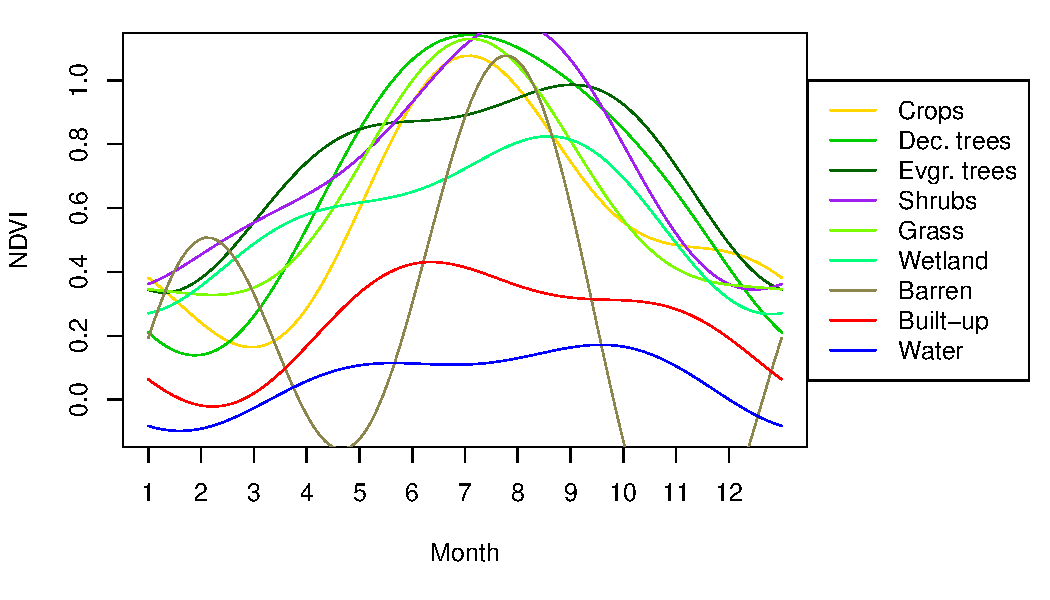
\includegraphics[width=0.9\textwidth]{thesis-figures/timeseries}
  \caption{NDVI variation through the year as fitted by harmonic models for each land cover class. The model parameters are mean harmonic parameters of endmember pixels.}
  \label{fig-timeseries}
\end{figure}

The covariates that were useful for all the classification methods (dropping them would always result in an increase in overall RMSE) were NIR, slope, mean NDVI and phase of both orders. This shows that it is beneficial for class separation to have all types of data: spectral, indices derived from spectral, parameters derived from elevation and time series parameters. Several covariates were correlated with each other: Red with blue (0.90), NIR with SWIR (0.76) and OSAVI with mean NDVI (0.93), so it was advantageous to drop one of the pair for algorithms sensitive to correlated data such as neural networks.

From the covariates, most important was mean NDVI. It is a good indicator of vegetation properties and especially helps to separate vegetation classes from water, built-up and barren cover (see also figure \ref{fig-timeseries}). Slope and NIR were useful for classification of every class as well. Slope particularly helped to determine the proportion of wetlands, which require flat terrain for water to stay; and it helped to determine the proportion of the water class itself, since the surface of open water is relatively flat. NIR at summer particularly helped to determine cultivated area and water fractions, as crops have very high reflectance in NIR during the peak of their growth, whereas water has low NIR throughout the year. LSWI, red and \nth{1} order amplitude helped to distinguish between all classes, with none standing out in particular. SWIR also helped overall, but it was particularly useful for water.

Some covariates were important for distinguishing particular classes. \nth{2} order amplitude was useful for discerning cultivated areas, as crops are harvested rather than allowed to grow naturally throughout the year, and may be harvested twice a year. \nth{2} order phase was useful for discerning wetlands, as their NDVI tends to start growing earlier in the year compared to other classes (see figure \ref{fig-timeseries}). TPI was most useful for shrubs, since their defining characteristic is height compared to trees. Since young trees less than 3 metres in height have been classified as shrubs, they tend to grow in between blocks of fully-grown trees in tree plantations. Hence at the extent of 100 m, a negative TPI indicates a dip in tree canopy height between adjacent blocks and allows identification of blocks of such short woody vegetation.

The inclusion of LSWI benefited the prediction of wetlands the most compared to other classes. Mean NDVI was also very useful for wetlands prediction. This is in line with the findings of \citet{davranche2010wetland}, \citet{dong2014lswi} and \citet{zhao2009indices}. The authors of the latter two studies also recommend using a ratio or difference of a vegetation index (such as NDVI) and a water index (such as LSWI), though the use of decision trees as in \citet{davranche2010wetland} makes it unnecessary.

The two least useful covariates were the water mask and aspect. The water mask was not useful due to three reasons: it is not accurate enough, as it does not mark inland waters and water on shallow shores as water; it is a binary mask, so it does not give any indication of how much of the pixel is covered by water; and there are other indicators of water available that are more accurate, such as slope and mean NDVI. Aspect was also of little use in the study area, as it is predominantly flat. Slopes in the area are mostly around local phenomena, such as river banks, and the pixel size was too large to capture such short-range variation in a way that the aspect metric would be meaningful. For hilly areas where the slopes do not have as much spatial variation, they are gentle enough that their aspect does not influence land cover. \nth{1} order phase was also less useful, since it has little variation and tends to be close to $\pi{}$, indicating an increase in NDVI in the summer and decrease in winter, which is true for most classes (see figure \ref{fig-timeseries}). It is true even for the evergreen tree class, since the trees are more likely to be covered in snow in winter. \nth{1} order phase was only useful for built-up and barren classes, which have little and erratic variation in NDVI over the year, and cultivated areas, whose \nth{1} order phase depends on the strong \nth{2} order harmonics. Note that even though the barren class appears to have strong variation in NDVI over the year, it is rather an artefact of the PROBA-V cloud mask misclassifying barren areas as clouds, resulting in very few data points from which to derive the harmonic parameters.

The inclusion of vegetation indices improved prediction accuracy, which is in line with \citet{Pelletier2016hardrf}. However, the authors of that study also noted that covariates derived from time series (start of season) did not improve prediction accuracy when the time series itself was included as a covariate. \citet{davranche2010wetland} and \citet{dong2014lswi} also noted that including the values of spectral bands or vegetation indices at specific periods of time as covariates was beneficial for prediction accuracy. While it would be valuable to compare the importance of such extra covariates, that was out of scope for this thesis. Such values do not change much between consecutive periods of time, which makes them correlated. The number of such extra covariates would also be large (depending on the time step chosen). This would in turn complicate the model term selection process. In addition, the problem of missing values would occur due to frequent cloud cover. A possible way to make use of this extra information in separate studies would be to make composite images over several months, or to interpolate values in the time series. Including soil and climate covariates could also further improve classification accuracy. However, this type of data has to be gathered using point measurements, so value interpolation would need to be used in order to make use of such data when making spatially extensive predictions.

\section{Recommendations}

Fuzzy land cover classification has the advantage that it can be suited to particular user needs as well as converted into hard classification (see figure \ref{fig-hard-rf}). Operations like that can be done much faster compared to rerunning the whole prediction process, since the most common case of hardening a fuzzy classification involves a simple maximum value calculation. In addition, proportion thresholds can be applied for classes that are either more or less important to a given user, yielding different hard classification maps depending on the needs of the user. If there are land cover classes that are not relevant to the user, it is likewise simple to drop the unwanted layers before performing the hardening operation.

\begin{figure}
  \begin{subfigure}{0.48\textwidth}
    \centering
    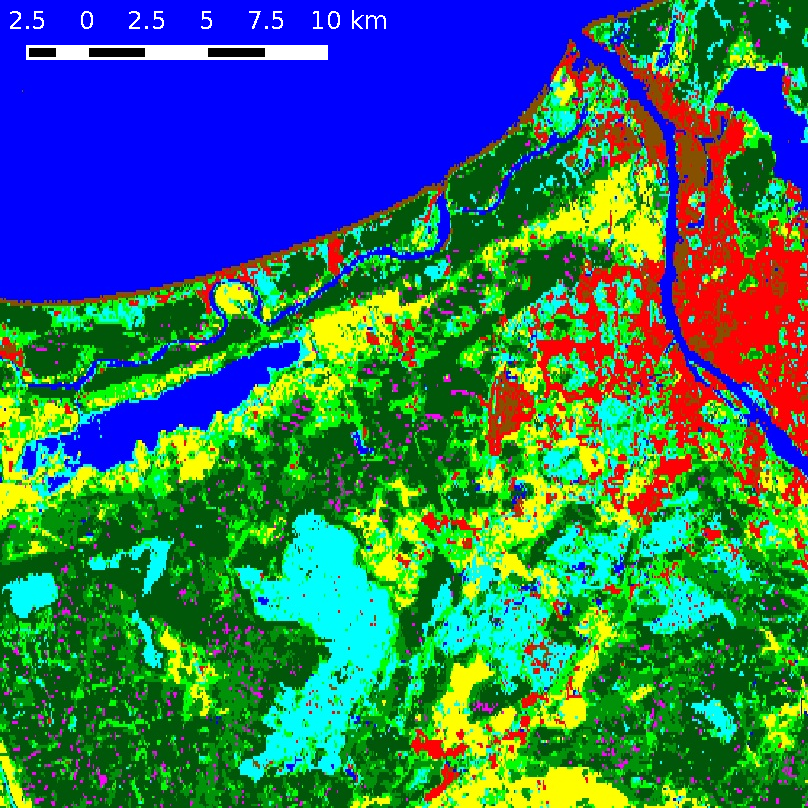
\includegraphics[width=\textwidth]{thesis-figures/figures-qgis/riga-hard-rf}
    \caption{Hardened random forest regression prediction}
  \end{subfigure} \hfill
  \begin{subfigure}{0.48\textwidth}
    \centering
    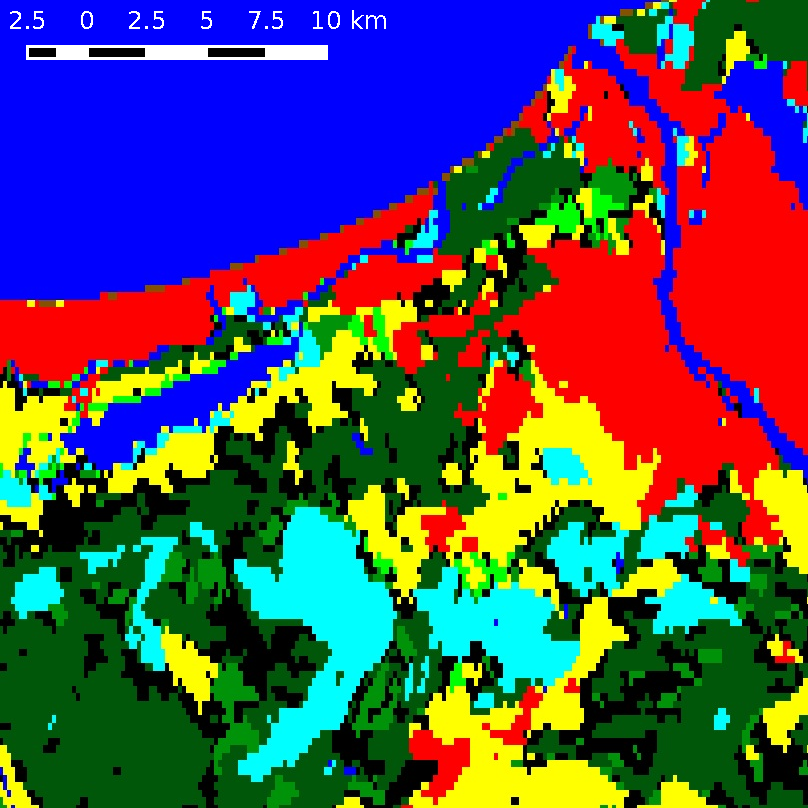
\includegraphics[width=\textwidth]{thesis-figures/figures-qgis/riga-hard-cci}
    \caption{LC-CCI classification, 2010 \citep{lccciguide}}
  \end{subfigure}
  \caption{Hard land cover classification of R\={\i}ga and its surroundings. Yellow: cultivated land; dark green: evergreen trees; green: deciduous trees; magenta: shrubs; light green: grass; brown: barren; teal: wetland; red: built-up area; blue: water; black: mixed pixels with no dominant class.}
  \label{fig-hard-rf}
\end{figure}

Increasing the number of ground truth samples and sample sites would increase the accuracy of prediction results, since there would be more samples to train the models on. In addition, none of the tested algorithms are spatially-aware. Given a sufficient number and fitting distribution of sampling sites to determine a semivariogram, adjustments to the algorithms could be made so that the predictions follow the observed spatial variation (i.e. pixels close to one another tend to have similar class proportions). This could improve the prediction accuracy and eliminate the salt-and-pepper effect. Such a modification was suggested by \citet{gong2013improvedcmeans} for fuzzy \textit{c}-means. The binary relevance method also allows for optimising the covariates for each class specifically, which could improve the classification accuracy per class. In addition, if global classification is desired, separate models per biome would give better results due to differences in indicators for land cover (for instance, seasonal changes are inverted in the southern hemisphere).

If ground truth is collected using manual interpretation, high resolution imagery in summer, autumn and winter, and especially panoramic photos and 3D models derived from photogrammery data help to identify land cover proportions with higher confidence. Drawing polygons to define the extent of land cover (as done in this study) takes more effort compared to subdividing a pixel into a grid and classifying the cells of the subgrid (as done in the case of \citet{perger2012geowiki}), but also results in more accurate ground truth data because border effects are eliminated. It also allows for identifying individual trees, which is crucial for properly identifying proportions of trees in mixed forests.

Additional covariates could help improve the separability of different classes. Soil properties, for instance, could improve the separability of vegetation classes, cultivated, barren and built-up areas. Since soil is important for vegetation nutrient uptake, it could also help discern between the vegetation classes. Additional time series parameters, such as separate  harmonic parameters for each separate spectral band, additional vegetation indices such as a ratio between NDVI and LSWI, and phenological parameters such as length of season could also give more opportunities for class separation. Including the time series itself as a set of covariates might increase prediction accuracy even more \citep{Pelletier2016hardrf}. Spectral band or vegetation index values during times of critical transition (such as in winter or autumn) could also help separate classes such as wetlands \citep{davranche2010wetland}. The classes that would benefit from more separability are grass, shrubs and cultivated areas. Shrubs are difficult to discern from trees using remote sensing, since their differentiating factor is height relative to ground height; this would require a dataset of canopy height. Discerning between grass and cultivated areas depends on the crop type; NDVI values shortly after harvest date would be a helpful covariate in this case.

Even though the inclusion of more covariates would help improve classification accuracy, it has to be balanced with the increase in processing time, which can be severe due to the curse of dimensionality \citep{Pelletier2016hardrf}. So it is also important to determine the covariates that contribute to classification accuracy the most, and drop those that contribute little, as correlated or irrelevant covariates have the potential to reduce prediction accuracy \citep{walton2008subpixelrf}. Due to a large number of potential covariates, combined with the big data nature of global land cover classification, additional studies dedicated to this topic are needed.

Model training and prediction tasks are largely multithreaded or can be made multithreaded with little effort, therefore running the process on a system with a large number of threads helps to minimise the wall clock time needed for the tasks to run. Moreover, there should also be a sufficient amount of memory (at least a gigabyte) available for each thread, due to the large number and size of covariate rasters. The raster chunk size should be set in a way that as much memory is used as possible while not going over the total amount of memory available, to decrease disk input/output operations and thus increase processing speed.

While the \textit{R} programming language is useful for the wealth of packages available for it and the ease of data visualisation, some packages used in this study were difficult to work with. During the analysis phase of the thesis, the \texttt{probaV} package had to be modified to work with PROBA-V Collection 1 data and to have a separate output function for cloud masking based on time series outliers. A separate function for selecting good quality pixels was also made for it. The package still lacks the ability to adapt the processing workflow to a given computer in order to avoid out-of-memory errors and does not always process data in a way that is both fast and conserves memory, without having to resort to modifying function parameters by trial-and-error. Furthermore, the \texttt{spfkm} function of the \texttt{gsif} package that implements the fuzzy \textit{c}-means algorithm is unable to handle data in the widespread \texttt{Raster} class format directly. In order to work around this limitation, the input data had to be converted into a \texttt{SpatialPixelsDataFrame}, which is not memory-safe and inefficient if the input data is not sparse. In addition, the \texttt{spfkm} function is implemented purely in \textit{R} at the moment, and without any built-in multithreading, which results in slower performance. These are all opportunities for improving the packages in the future, which would enable broader use of PROBA-V data and faster fuzzy \textit{c}-means classification, respectively.

In this study, it was assumed that land cover classes do not change over the period of the last 3 years. In reality this may not always be the case, and thus recent changes such as deforestation may not be reflected in the classification results. Given enough samples to make it feasible, an approach for identifying breaks in time series such as BFAST \citep{Verbesselt2010bfast} could loosen this assumption and improve the classification accuracy when aiming to produce a land cover map representing a particular year.

To obtain robust time series parameters, a large enough number of cloud-free observations over the year are needed. While the PROBA-V satellite has a frequent revisit time, much of the imagery is affected by clouds or cloud shadows, which are difficult and time-consuming to filter out due to cloud masks provided by VITO having cloud and cloud shadow detection problems. The cloud detection algorithm has been improved in Collection 1, but it still does not detect cloud shadows well enough and tends to mistake bright barren areas for clouds. This results in visible artefacts in affected areas. In addition, longer time series would result in more frequent cloud-free observations, which would make the time series more robust as well. However, it would also increase the chance of land cover change happening in any given pixel, which would have the opposite effect of making the time series less robust.

While PROBA-V data is useful for making use of time series due to fast revisit time and consistent pixel locations, the land cover classification accuracy could be further improved by making use of data from recent missions such as Sentinel-2. The multi-spectral instrument (MSI) of Sentinel-2 provides imagery at a resolution as fine as 10 by 10 metres, and includes even 13 spectral bands including red edge \citep{gatti2016sentinel2}. The footprints of finer resolution pixels are more likely to represent a single land cover class, increasing the proportion of endmember pixels compared to mixed pixels. Despite that, mixed pixels would still make up a large portion of all pixels, especially in heterogeneous areas such as mixed forests and towns. Whether or not fuzzy classification would be more useful than hard in that case would have to be investigated separately. In addition, finer resolution also comes with the drawback of increased processing time and storage requirements. A single computer would no longer be sufficient for such a task, but a possible solution would be cluster computing. Sentinel-2 also has a longer revisit time compared to PROBA-V (5 days as opposed to 2 days), which increases the likelihood of the surface being obscured by clouds during the overpass. One solution to that problem would be multisensor fusion, which usually results in an increase in classification accuracy \citep{yu2014metadiscoveries}.

In comparison, the fuzzy classification approach is more readily applicable to data from the OLCI instrument of the Sentinel-3 mission. Sentinel-3 satellites will have a revisit time of 2 days, and the pixel resolution of the OLCI instrument is 300 by 300 metres \citep{Donlon2012sentinel3}. This resolution is relatively coarse, so there would be a large number of mixed pixels, making fuzzy classification more important to use, but also the coarser resolution would inevitably lead to a decrease in classification accuracy. It also does not yet have a long enough time series to derive temporal metrics from. All in all fuzzy classification can also be performed on data provided by recent missions such as Sentinel-2 and Sentinel-3; which one is best suited depends on the desired end product and data processing capabilities. Multisensor fusion is also an option that could be explored, especially if the goal is to obtain the best classification accuracy at a relatively smaller scale, such as a region or continent.

\chapter{Conclusion}

The land cover class proportion prediction accuracy of all tested fuzzy classification methods was similar, once the models were optimised by dropping unnecessary covariates and adjusting model parameters. Random forest regression using the binary relevance method was the most accurate method (MAE: 11.7, RMSE: 20.8), but it was not significantly more accurate than fuzzy \textit{c}-means (MAE: 12.0, RMSE: 22.1) and neural networks (MAE: 12.7, RMSE: 22.1). Thus the selection of a fuzzy classification method is not as important as the selection of model covariates. Visual inspection of the prediction results showed that all of the methods are capable of predicting land cover well. The gradient from deciduous to evergreen trees was well visible looking at the whole-tile prediction result of each method. Wetlands were identified well, with sharp shift to other classes on the edges, which is typical of the study area, except for peat extraction sites which tended to be confused with barren and built-up classes.

The covariates of all four types (spectral bands, vegetation indices, terrain metrics and time series metrics) were important for increasing the prediction accuracy in all classification methods tested. Mean NDVI over the whole year was the most important covariate. From the spectral bands, near infrared was the most important, followed by red and shortwave infrared. Slope was the most important terrain metric, and the amplitude of the \nth{1} order harmonics was the most important temporal metric. \nth{2} order amplitude was important for predicting the proportion of cultivated land in particular, \nth{2} order phase was important for wetland prediction, terrain positioning index was important for shrub prediction. Least important covariates were the aspect of the slope and the water mask.

Random forest regression had much longer prediction times (20.5 hours) than the other fuzzy classification methods. Prediction speed seems to be a tradeoff for accuracy with all tested methods, with fuzzy \textit{c}-means being much faster to predict than random forest regression (42 minutes), but giving a less accurate prediction, and neural networks in turn being less accurate but faster than fuzzy \textit{c}-means (25 minutes).

% Fully fuzzy approaches (fuzzy c-means, neural networks) are not necessarily more accurate than partially fuzzy binary relevance methods, but are faster.

Training the models only on endmember pixels, as was done with multiclass gradient boosting, introduces problems with model optimisation, as the predictions of such models are by default less fuzzy than the reality. In addition, it becomes difficult to compare such methods with those that can use mixed pixels for training due to differences in training sample size. Therefore when mixed pixels are available for training, techniques that allow making use of such pixels should be used. Running the algorithm in regression mode and using the binary relevance technique, as was the case for random forest, appears to be a good solution in terms of classification accuracy, although the processing time is much longer.

Given the recent advances in remote sensing technology (such as the Sentinel-2 and Sentinel-3 missions), there is a potential to further increase the accuracy of fuzzy classification by leveraging higher spatial and spectral resolution data, while making use of the same fuzzy classification methods. However, the increase in data quantity would result in longer processing times. One solution would be to make use of and increase the processing power of virtual machines provided by the data provider (such as PROBA-V MEP or Sentinel Cloud Toolbox), or to focus on land cover of a smaller area than the entire globe.

\bibliography{bibliography}

\begin{appendices}

 \chapter{Visual interpretation data sources}
 \label{app-layerlist}
 \begin{table}[!ht]
  \begin{center}
    %\resizebox{\textwidth}{!}{
      \begin{tabular}{llrl}
	\hline
	Layer provider & Layer type & Year & URL \\
	\hline
	ESA LC-CCI & Land cover & 2010 & \url{http://maps.elie.ucl.ac.be/CCI/viewer} \\
	OpenStreetMap & Topographical & 2016 & \url{http://www.openstreetmap.org} \\
	Google & Satellite & ?-2016 & \url{https://www.google.com/maps} \\
	Google & Panoramic & 2009-2016 & \url{https://www.google.com/maps} \\
	Bing & Satellite & ?-2016 & \url{https://www.bing.com/maps} \\
	Yandex & Satellite & ?-2016 & \url{https://yandex.com/maps/} \\
	Yandex & Panoramic & ?-2016 & \url{https://yandex.com/maps/} \\
	Lithuania & Topographical & 2016 & \url{http://www.geoportal.lt} \\
	Lithuania & Orthophoto & 2005-2015 & \url{http://www.geoportal.lt} \\
	Latvia & Orthophoto & 2010-2011 & \url{http://www.lgia.gov.lv} \\
	Latvia & Orthophoto & 2010 & \url{http://www.gisnet.lv/cgi-bin/osm_latvia} \\
	Estonia & Topographical & 2016 & \url{http://geoportaal.maaamet.ee} \\
	Estonia & Orthophoto & 2007-2009 & \url{http://geoportaal.maaamet.ee} \\
	Finland & Topographical & 2016 & \url{http://kartat.kapsi.fi} \\
	Finland & Orthophoto & 2006-2016 & \url{http://kartat.kapsi.fi} \\
	\hline
      \end{tabular}
    %}
  \end{center}
  \caption{List of layers used to aid visual interpretation when gathering ground truth data. Most of the layers were accessed as WMS or TMS services (exceptions: Google Street View and Yandex accessed through a web interface; Google and Bing satellite data accessed using JavaScript API).}
  \label{tbl-layers}
 \end{table}
 
 \chapter{Land cover class relation to LC-CCI}
 \label{appendix-classes}
 \begin{table}[!ht]
  \begin{center}
    %\resizebox{0.6\textwidth}{!}{
    \begin{adjustbox}{totalheight=\textheight-13\baselineskip}
      \begin{tabular}{lp{10.5cm}l}
	\hline
	Class in this study & Equivalent classes in LC-CCI and their digital numbers & \\
	\hline
	\multirow{4}{*}{Cultivated} & Cropland rainfed & 10 \\
	  & Cropland rainfed - Herbaceous cover & 11 \\
	  & Cropland rainfed - Tree or shrub cover & 12 \\
	  & Cropland irrigated or post-flooding & 20 \\
	  & Mosaic cropland (>50\%) / natural vegetation (tree / shrub / herbaceous cover) (<50\%) & 30 \\
	\hline
	\multirow{7}{*}{Deciduous trees} & Tree cover  broadleaved  deciduous  closed to open (>15\%) & 60 \\
	  & Tree cover  broadleaved  deciduous  closed (>40\%) & 61 \\
	  & Tree cover  broadleaved  deciduous  open (15-40\%) & 62 \\
	  & Tree cover  needleleaved  deciduous  closed to open (>15\%) & 80 \\
	  & Tree cover  needleleaved  deciduous  closed (>40\%) & 81 \\
	  & Tree cover  needleleaved  deciduous  open (15-40\%) & 82 \\
	  & Tree cover  mixed leaf type (broadleaved and needleleaved) & 90 \\
	\hline
	\multirow{4}{*}{Evergreen trees} & Tree cover broadleaved evergreen closed to open (>15\%) & 50 \\
	  & Tree cover  needleleaved  evergreen  closed to open (>15\%) & 70 \\
	  & Tree cover  needleleaved  evergreen  closed (>40\%) & 71 \\
	  & Tree cover  needleleaved  evergreen  open (15-40\%) & 72 \\
	\hline
	\multirow{4}{*}{Shrubs} & Mosaic tree and shrub (>50\%) / herbaceous cover (<50\%) & 100 \\
	  & Shrubland & 120 \\
	  & Shrubland evergreen & 121 \\
	  & Shrubland deciduous & 122 \\
	\hline
	\multirow{4}{*}{Grass} & Grassland & 130 \\
	  & Lichens and mosses & 140 \\
	  & Mosaic herbaceous cover (>50\%) / tree and shrub (<50\%) & 110 \\
	  & Mosaic natural vegetation (tree/shrub/herbaceous cover) (>50\%) / cropland (<50\%) & 40 \\
	\hline
	\multirow{6}{*}{Barren} & Sparse vegetation (tree/shrub/herbaceous cover) (<15\%) & 150 \\
	  & Sparse shrub (<15\%) & 152 \\
	  & Sparse herbaceous cover (<15\%) & 153 \\
	  & Bare areas & 200 \\
	  & Consolidated bare areas & 201 \\
	  & Unconsolidated bare areas & 202 \\
	\hline
	\multirow{3}{*}{Wetland} & Tree cover flooded fresh or brakish water & 160 \\
	  & Tree cover flooded saline water & 170 \\
	  & Shrub or herbaceous cover flooded fresh/saline/brakish water & 180 \\
	\hline
	Built-up & Urban areas & 190 \\
	\hline
	Water & Water bodies & 210 \\
	\hline
      \end{tabular}
    %}
    \end{adjustbox}
  \end{center}
  \caption{List of classes used in this study and their relation with LC-CCI classes. The LC-CCI classes listed for each class in this study were merged in order to perform stratified random sampling for the first stage of ground truth sample selection.}
  \label{tbl-classes}
 \end{table}
 
 \chapter{Per-class errors}
 \section{Cross-validation}
 \begin{figure}[!h]
  \centering
  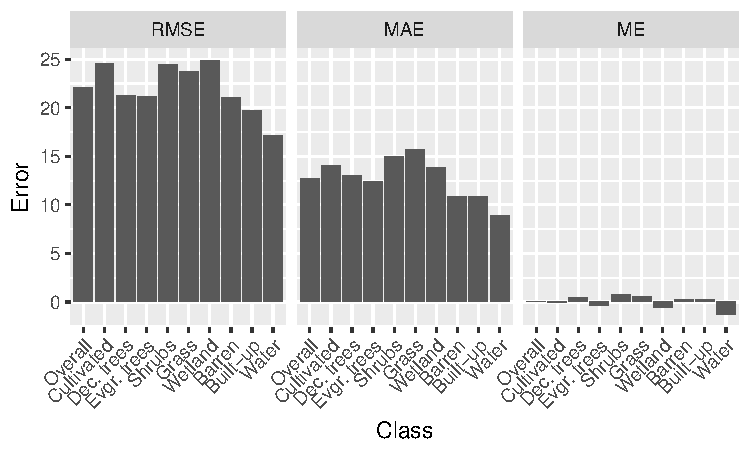
\includegraphics[width=0.75\textwidth]{thesis-figures/perclass-errors-nn}
  \caption{Errors per class using neural networks, 4-fold cross-validation. RMSE: root mean squared error, MAE: mean absolute error, ME: mean error.}
  \label{fig-perclass-errors-nn}
 \end{figure}
 \begin{figure}[!h]
  \centering
  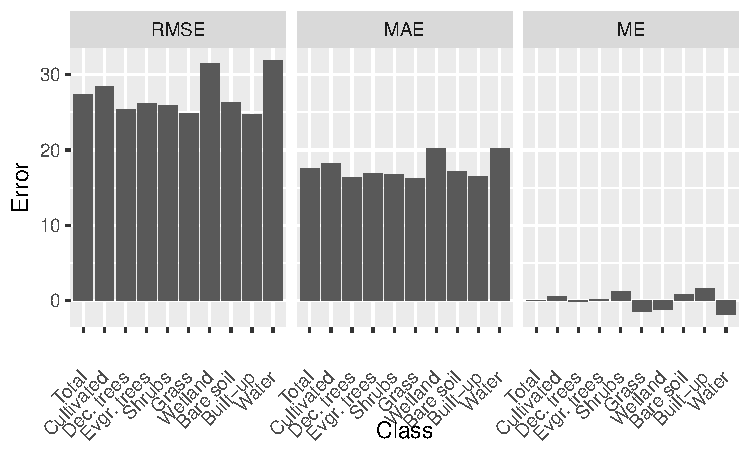
\includegraphics[width=0.75\textwidth]{thesis-figures/perclass-errors-ctrl}
  \caption{Errors per class if assigning equal proportions for each class (100\%/9). RMSE: root mean squared error, MAE: mean absolute error, ME: mean error.}
  \label{fig-perclass-errors-ctrl}
 \end{figure}
 
 \section{Mixed pixel validation}
 \begin{figure}[!h]
  \centering
  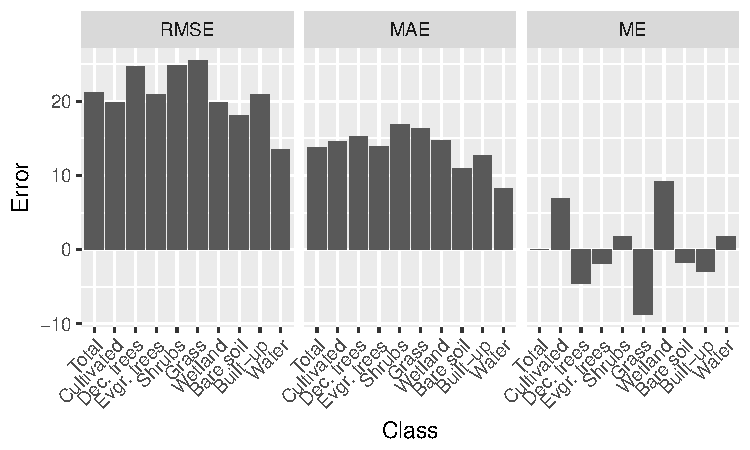
\includegraphics[width=0.75\textwidth]{thesis-figures/perclass-errors-gb}
  \caption{Errors per class using multiclass gradient boosting, trained on endmember pixels and validated on mixed pixels. RMSE: root mean squared error, MAE: mean absolute error, ME: mean error.}
  \label{fig-perclass-errors-gb}
 \end{figure}
 
 \chapter{Source code}
 The source code of the scripts used to perform the processing in this thesis is under the GNU General Public License version 3 or later. It can be publicly accessed via GitHub: \url{https://github.com/GreatEmerald/master-classification}
 
\end{appendices}

\end{document}
